\documentclass[11pt]{amsart}
\usepackage[margin=1.15in]{geometry}
\usepackage{amssymb,amsmath,mathtools}
\usepackage{graphicx,booktabs,array,float}
\usepackage[hidelinks]{hyperref}
\usepackage[expansion=false]{microtype}

\newtheorem{theorem}{Theorem}[section]
\newtheorem{proposition}[theorem]{Proposition}
\newtheorem{lemma}[theorem]{Lemma}
\newtheorem{corollary}[theorem]{Corollary}
\newtheorem{mainthm}{Theorem}
\renewcommand{\themainthm}{\Alph{mainthm}}
\newtheorem{maincor}[mainthm]{Corollary}
\theoremstyle{definition}
\newtheorem{definition}[theorem]{Definition}
\newtheorem{remark}[theorem]{Remark}
\newtheorem{example}[theorem]{Example}

\newcommand{\ZZ}{\mathbb{Z}}
\newcommand{\QQ}{\mathbb{Q}}
\newcommand{\RR}{\mathbb{R}}
\newcommand{\CC}{\mathbb{C}}
\newcommand{\HH}{\mathbb{H}}
\newcommand{\vt}{\vartheta}
\newcommand{\pf}{p_{24}}
\newcommand{\cF}{c^{F}}
\newcommand{\dstar}{d^{*}}
\newcommand{\Hc}{\mathcal{H}}
\newcommand{\Hh}{\widehat{\mathcal{H}}}
\newcommand{\Ah}{\widehat{A}}
\newcommand{\Mset}{\mathcal{M}}
\newcommand{\erfc}{\operatorname{erfc}}
\newcommand{\e}{\mathbf{e}}
\newcommand{\doi}[1]{\href{https://doi.org/#1}{\nolinkurl{doi:#1}}}
\newcommand{\zenodoCodeDOI}{10.5281/zenodo.24124994}

\setlength{\emergencystretch}{2.5em}
\hbadness=2000
\raggedbottom
\begin{document}

\title[Positivity of rotating black hole indices on K3]{Positivity of Rotating Black Hole\\ Indices on K3}

\author{Deep Bhattacharjee}
\address{Formerly, Electro-Gravitational Space Propulsion Laboratory (EGSPL), Bhubaneswar, Odisha 751030, India}
\address{Formerly, University of Calcutta (Heramba Chandra College), 23/49 Gariahat Road, Golpark, Kolkata 700029, West Bengal, India}
\email{d.bhattacharjee@erl-forschung.de}
\email{itsdeep@live.com}
\email{egspl@proton.me (GitHub-related contact; GitHub account creelie)}
\urladdr{https://orcid.org/0000-0003-0466-750X}

\begin{abstract}
We prove Sen's conjecture that single-centred rotating black holes in type~IIB string theory on $K3\times S^1$ have a positive index at fixed angular momentum, for every charge of discriminant at most $7200$ and for all charges whose D1--D5 product is $1$ or a prime power below $32$.

\medskip\noindent\textbf{Keywords:} black hole microstates; mock Jacobi forms; Rademacher expansion.

\smallskip\noindent\textbf{MSC 2020:} 11F50 (primary); 11F37, 11F30, 81T30, 83E30.
\end{abstract}

\maketitle

\section{Introduction}\label{sec:intro}

Strominger and Vafa explained the entropy of a five-dimensional supersymmetric black hole by counting the bound states of D1-branes, D5-branes and momentum on $K3\times S^1$ \cite{SV96}, and Breckenridge, Myers, Peet and Vafa extended the count to black holes that rotate \cite{BMPV97}. The number that is computed at weak coupling is an index: states are weighted by a sign, so that the result is protected when the coupling grows and the black hole forms. Dijkgraaf, Verlinde and Verlinde found the generating function of these indices for type~II string theory on $K3\times T^2$: it is the reciprocal of the Igusa cusp form $\Phi_{10}$ of genus two \cite{DVV97}. Through the relation between four- and five-dimensional black holes found by Gaiotto, Strominger and Yin \cite{GSY06}, the same function governs the rotating black holes on $K3\times S^1$.

The integers obtained in this way count all bound states, not only the black hole. Some of them are bound states of two black holes held apart by electromagnetic forces, and some are modes that live outside the horizon. Sen showed that once both are removed, what remains is the index of the horizon itself, and he argued that this index must be positive: a supersymmetric single-centred black hole in four dimensions is spherically symmetric, so its microstates carry zero angular momentum and contribute to the index with the same sign \cite{Sen11,DGMS11}. For the rotating black holes of five dimensions he defined the index at fixed angular momentum, which removes the multiplicities coming from rotations of the horizon, and conjectured that it too is positive \cite{Sen12}. Bringmann and Murthy turned these predictions into precise statements about Fourier coefficients and proved them when the D1--D5 product $m=Q_1Q_5$ equals $1$ or $2$ \cite{BM13}.\footnote{Bringmann and Murthy give two proofs for $m=2$, one by the circle method and one by explicit identities between theta functions, Eisenstein series and class numbers \cite[\S\S4--6]{BM13}. They state the fixed angular momentum conjecture in \cite[\S2.3]{BM13}, attributing it to \cite{Sen12}.}

This paper proves the conjecture at fixed angular momentum for every charge of discriminant at most $7200$, and for all charges when $m$ is $1$ or one of the seventeen prime powers below $32$.\enlargethispage{6pt}

\subsection*{The indices}
Throughout, $\tau$ lies in the upper half-plane $\HH$, $z\in\CC$, $y=\operatorname{Im}\tau$, $\e(x)=e^{2\pi ix}$, $q=\e(\tau)$ and $\zeta=\e(z)$. Let $\Delta=q\prod_{n\ge1}(1-q^n)^{24}$, and let $\pf(k)$ be the number of partitions of $k$ into parts of $24$ colours, so that $\Delta^{-1}=\sum_{k\ge0}\pf(k)q^{k-1}$. Let
\[
A(\tau,z)=(\zeta-2+\zeta^{-1})\prod_{n\ge1}\frac{(1-q^n\zeta)^2(1-q^n\zeta^{-1})^2}{(1-q^n)^4}
\]
be the weak Jacobi form $\phi_{-2,1}$ of weight $-2$ and index $1$, and let $\phi_{0,1}$ be the weak Jacobi form of weight $0$ and index $1$ normalised by $\phi_{0,1}(\tau,0)=12$; the elliptic genus of a K3 surface is $2\phi_{0,1}$ \cite[\S9]{EZ85}, \cite{DMVV97}. Define weak Jacobi forms $\chi_N$ of weight $0$ and index $N$ by
\begin{equation}\label{eq:dmvv}
\sum_{N\ge0}\chi_N(\tau,z)\,p^N=\exp\Bigl(\sum_{k\ge1}p^k\,(2\phi_{0,1})\big|V_k\,(\tau,z)\Bigr),
\end{equation}
where $V_k$ is the Hecke operator of weight $0$ recalled in Section~\ref{sec:jacobi}; by the theorem of Dijkgraaf, Moore, Verlinde and Verlinde, $\chi_N$ is the elliptic genus of the symmetric product $\mathrm{Sym}^N(K3)$ \cite{DMVV97}. For $m\ge-1$ put
\begin{equation}\label{eq:psim}
\psi_m=\frac{\chi_{m+1}}{\Delta\,A}.
\end{equation}
These are the coefficients of the expansion $1/\Phi_{10}=\sum_{m\ge-1}\psi_m(\tau,z)\,\e(m\sigma)$ in the third variable of the Siegel upper half-space \cite[\S3.1]{BM13}. The function $\psi_m$ has double poles at the points $z\in\ZZ\tau+\ZZ$, and its Fourier coefficients depend on where it is expanded; this dependence is the wall crossing of two-centred black holes. Following Dabholkar, Murthy and Zagier as presented in \cite[\S3.1]{BM13}, one removes the poles with the Appell--Lerch sum
\begin{equation}\label{eq:appell}
A_{1,m}(\tau,z)=\sum_{s\in\ZZ}\frac{q^{ms^2+s}\zeta^{2ms+1}}{(1-q^s\zeta)^2},
\end{equation}
and puts
\begin{equation}\label{eq:psiF}
\psi^F_m=\psi_m-\frac{\pf(m+1)}{\Delta}\,A_{1,m}=\sum_{n\ge-1}\sum_{l\in\ZZ}\cF_m(n,l)\,q^n\zeta^l .
\end{equation}
The function $\psi^F_m$ is holomorphic in $z$ (Lemma~\ref{lem:poles}), so its coefficients $\cF_m(n,l)$ are well defined. They are integers with $\cF_m(n,l)=\cF_m(n,-l)$, and $\cF_m(n,l)$ depends only on $4mn-l^2$ and on $l$ modulo $2m$.

A four-dimensional charge is described by three integers $(n,l,m)$, the T-duality invariants $Q^2/2$, $Q\cdot P$ and $P^2/2$ of the electric and magnetic charge vectors, and its discriminant is $D=4mn-l^2$. A single-centred black hole exists only for $D>0$, and its horizon area is then $4\pi\sqrt{D}$ in Planck units, so that its entropy is $\pi\sqrt D$. To the charge belongs the positive definite binary quadratic form $nX^2+lXY+mY^2$. Every such form is equivalent under $\mathrm{GL}_2(\ZZ)$ to exactly one form $aX^2+bXY+cY^2$ with $0\le b\le c\le a$ (Lemma~\ref{lem:reduced}), and we call $(a,b,c)$ the reduced form of $(n,l,m)$. The \emph{single-centred index} is
\begin{equation}\label{eq:dstar}
\dstar(n,l,m)=\begin{cases}(-1)^{b+1}\,\cF_c(a,b), & D>0,\\ 0,& D\le0,\end{cases}
\end{equation}
and Section~\ref{sec:physics} explains why this is the index of the horizon. For the five-dimensional black hole with momentum $n$, angular momentum $J_{3L}=J/2$ and D1--D5 product $m=Q_1Q_5$, the index at fixed angular momentum is \cite{Sen12}, \cite[\S2.3, \S3.1]{BM13}
\begin{equation}\label{eq:drot}
d(n,J,m)=\dstar(n,J,m)-\dstar(n,J+2,m),\qquad J\ge0 .
\end{equation}
The conjecture of Sen is that $d(n,J,m)>0$ whenever $4mn-J^2>0$; it contains the four-dimensional statement $\dstar>0$ as the special case in which the second term vanishes.

\subsection*{Results}
Let $\Mset=\{1,2,3,4,5,7,8,9,11,13,16,17,19,23,25,27,29,31\}$ be the set consisting of $1$ and the prime powers below $32$.

\begin{mainthm}[Charges of small discriminant]\label{thm:A}
For every charge with $0<4mn-l^2\le7200$ the single-centred index $\dstar(n,l,m)$ is positive, and for every five-dimensional charge with $0<4mn-J^2\le7200$ the index $d(n,J,m)$ at fixed angular momentum is positive.
\end{mainthm}

\begin{mainthm}[Fixed angular momentum]\label{thm:B}
Let $m\in\Mset$. Then $d(n,J,m)>0$ for all integers $n$ and $J\ge0$ with $4mn-J^2>0$.
\end{mainthm}

\begin{maincor}\label{cor:C}
If the reduced form $(a,b,c)$ of a charge $(n,l,m)$ with $4mn-l^2>0$ has $c\in\Mset$, then $\dstar(n,l,m)>0$.
\end{maincor}

The proof of Theorem~\ref{thm:B} needs an exact description of the mock modular nature of $\psi^F_m$. Let $H(N)$ be the Hurwitz class number of positive definite binary quadratic forms of discriminant $-N$, counted with weight $1/2$ and $1/3$ for forms equivalent to multiples of $X^2+Y^2$ and $X^2+XY+Y^2$, with $H(0)=-1/12$ and $H(N)=0$ for $N<0$ or $N\equiv1,2\pmod 4$. Let $\Hc(\tau,z)=\sum_{n,l}H(4n-l^2)q^n\zeta^l$, and let $\Hc|V_m$ be its image under the Hecke operator of weight $2$, whose coefficients are
\begin{equation}\label{eq:HVm}
h_m(n,l)=\sum_{d\mid(m,n,l)}d\,H\Bigl(\frac{4mn-l^2}{d^2}\Bigr).
\end{equation}
For an integer $e\ge1$ let $\Phi|U_e$ denote the function $\Phi(\tau,ez)$; it multiplies the index by $e^2$. Define the class number term $\mathcal G_m$ for $m=1$ and for prime powers $m=p^k$ by
\begin{equation}\label{eq:Gm}
\mathcal G_1=\Hc,\qquad \mathcal G_p=\Hc|V_p,\qquad \mathcal G_{p^k}=\Hc|V_{p^k}-p\,(\Hc|V_{p^{k-2}})|U_p\quad(k\ge2),
\end{equation}
so that its coefficients are $g_m(n,l)=h_m(n,l)$ for $m=1$ or $m$ prime, and $g_m(n,l)=h_m(n,l)-p\,h_{m/p^2}(n,l/p)$ for $k\ge2$, where the second term is read as $0$ unless $p\mid l$. Put $\lambda_1=648$ and $\lambda_m=\pf(m+1)$ for a prime power $m$.

\begin{mainthm}[The class number term]\label{thm:D}
For $m=1$ and for every prime power $m$, the function
\[
\phi_m=\Delta\,\psi^F_m+\lambda_m\,\mathcal G_m
\]
is a weak Jacobi form of weight $2$ and index $m$. For $m\in\{1,2,3,5,7,11,13\}$ it is the polynomial in $E_4,E_6,A,\phi_{0,1}$ listed in Appendix~\ref{app:data}; in particular $\phi_1=3E_4A$ and $\phi_2=\frac13(22E_4A\phi_{0,1}-10E_6A^2)$.
\end{mainthm}

For $m=1,2$ Theorem~\ref{thm:D} is the pair of identities \cite[(3.6), (3.7)]{BM13}. The class number term comes out of the proof: it is the combination of Hecke images of $\Hc$ whose nonholomorphic completion cancels that of $A_{1,m}$. The value $\lambda_1=2\pf(2)$, rather than $\pf(2)$, reflects the fact that the operator $V_p$ doubles the shadow of $\Hc$ while $V_1$ does not. For $m=p^k$ with $k\ge2$ the shadow of $\Hc|V_{p^k}$ is too large by the contribution of the lattice vectors divisible by $p$, and $p\,(\Hc|V_{p^{k-2}})|U_p$ removes exactly this contribution (Lemma~\ref{lem:count}). When $m$ has two distinct prime factors no combination of the functions $\Hc|V_{m/e^2}|U_e$ has the right shadow (Section~\ref{sec:remarks}).

\subsection*{What the proof has to overcome}
Three features make the problem harder than its four-dimensional analogue in $\mathcal N=8$ string theory, where the index is a finite combination of coefficients of a single weak Jacobi form.

First, the coefficients $\cF_m(n,l)$ themselves are not positive in the required sense. For $m=5$ the charge $(n,J)=(10,14)$ has discriminant $4$, and the coefficient of $\psi^F_5$ at this discriminant gives $(-1)^{14+1}\cF_5(10,14)=-2\,023\,536$; the reduced form of $(10,14,5)$ is $(1,0,1)$, and $\dstar(10,14,5)=-\cF_1(1,0)=50\,064$. The passage to the reduced form in \eqref{eq:dstar} is therefore essential, and it has the consequence that the two terms of \eqref{eq:drot} can be coefficients of two different functions $\psi^F_c$.

Second, $\psi^F_m$ is not modular: it is the sum of a weakly holomorphic Jacobi form and a multiple of $\Hc|V_m/\Delta$. The main term of the asymptotic formula comes from the first, but the class numbers contribute an error that is only polynomially smaller in the range that matters for $m\le5$.

Third, the positivity of $d(n,J,m)$ is a statement about a difference of two exponentially large numbers. When $J$ is small the two discriminants $D$ and $D-4(J+1)$ are close, and the main terms differ by a factor $1-O(D^{-1/2})$. The error terms have to be smaller than this relative gap, uniformly, and they are controlled only beyond an explicit discriminant $D^*_m$ that ranges from $258$ to $7052$.

\subsection*{Plan}
Section~\ref{sec:physics} recalls where the formula \eqref{eq:drot} comes from. Section~\ref{sec:forms} proves the facts about binary quadratic forms that the reduction needs, in particular a lemma on successive minima that controls the second charge $(n,J+2,m)$. Section~\ref{sec:jacobi} defines the Jacobi forms and proves that $\psi^F_m$ is holomorphic, elliptic and even, and that its most polar coefficient is $m+2$. Section~\ref{sec:completion} proves Theorem~\ref{thm:D} from Zwegers' completion of Appell--Lerch sums and Zagier's completion of the class number generating function. Section~\ref{sec:rademacher} gives the exact formula for the coefficients of $\phi_m/\Delta$, Section~\ref{sec:bessel} proves the inequalities for Bessel functions that are needed, and Section~\ref{sec:tail} proves the tail estimate: beyond $D^*_m$ the index grows faster than its error. Sections~\ref{sec:proofB} and~\ref{sec:proofA} prove Theorems~\ref{thm:B} and~\ref{thm:A} and Corollary~\ref{cor:C}, and Section~\ref{sec:remarks} discusses what lies beyond. Appendix~\ref{app:data} lists $\phi_m$ and the polar coefficients, Appendix~\ref{app:computation} describes the exact computations, and Appendix~\ref{app:bounds} proves the elementary bounds for $H(N)$ and $\pf(k)$.

K3 surfaces, their involutions and the Calabi--Yau threefolds fibred by them are studied in \cite{Bha22,BN26}, and the heterotic and M-theory compactifications to which type~II strings on K3 are dual in \cite{SBBT26}.

\section{Black holes and their indices}\label{sec:physics}

This section explains the formulae \eqref{eq:dstar} and \eqref{eq:drot}. Nothing in the proofs of Sections~\ref{sec:forms} to~\ref{sec:proofA} depends on it, and the reader interested only in the mathematics can take \eqref{eq:psiF}, \eqref{eq:dstar} and \eqref{eq:drot} as definitions.

\subsection{Four dimensions}\label{ssec:4d}
Type~IIB string theory on $K3\times S^1\times\widetilde S^1$ has $\mathcal N=4$ supersymmetry in four dimensions. Its charges form a vector $(Q,P)$ of electric and magnetic charges in two copies of an even lattice of signature $(6,22)$, and the duality group $\mathrm{SL}_2(\ZZ)\times O(6,22;\ZZ)$ acts on them. The T-duality invariants
\[
n=\tfrac12Q^2,\qquad l=Q\cdot P,\qquad m=\tfrac12P^2
\]
are integers, and the S-duality group $\mathrm{SL}_2(\ZZ)$ acts on the triple $(n,l,m)$ exactly as $\mathrm{SL}_2(\ZZ)$ acts on the coefficients of the binary quadratic form $nX^2+lXY+mY^2$ by linear substitutions of $(X,Y)$ \cite{Sen08r}. A quarter-BPS black hole with these charges exists when the discriminant $D=4mn-l^2$ is positive, and its entropy is then $\pi\sqrt D$.

The index computed by the microscopic theory is a helicity trace, the quantity that remains constant as the string coupling is increased until a black hole forms. For charges with torsion one, the indices of all states of charge $(n,l,m)$ are, up to the sign $(-1)^{l+1}$, the Fourier coefficients of $1/\Phi_{10}$ in the variables conjugate to $n$, $l$ and $m$ \cite{DVV97,Sen08r}. Because $1/\Phi_{10}$ has poles, these coefficients depend on the contour of integration, and the contour is determined by the moduli at infinity. The jumps across the poles are the indices of bound states of two black holes, which exist on one side of a wall in moduli space and not on the other \cite{Sen08r}.

The single-centred black hole is isolated by choosing the moduli at their attractor values, where no two-centred bound state exists. Dabholkar, Murthy and Zagier showed that for a charge with $0\le l\le m\le n$ the index at the attractor point is the coefficient of $\psi^F_m$; Bringmann and Murthy record this as \cite[\S3.1]{BM13}
\[
\dstar(n,l,m)=(-1)^{l+1}\cF_m(n,l)\qquad(0\le l\le m\le n,\ 4mn-l^2>0).
\]
The single-centred index does not depend on the moduli at infinity, so it is invariant under S-duality, which moves the moduli but not the attractor values belonging to a given charge. Every charge with $D>0$ is S-dual, up to the reflection $l\mapsto-l$, to a unique charge with $0\le l\le m\le n$ (Lemma~\ref{lem:reduced}); the reflection does not change the index because $\cF_m(n,-l)=\cF_m(n,l)$. This gives \eqref{eq:dstar} for $D>0$. A charge with $D\le0$ carries no single-centred black hole, and its single-centred index is zero.

\subsection{Five dimensions}\label{ssec:5d}
In type~IIB string theory on $K3\times S^1$, a system of $Q_5$ D5-branes wrapped on $K3\times S^1$ and $Q_1$ D1-branes wrapped on $S^1$, carrying $n$ units of momentum along $S^1$, forms a supersymmetric black hole in five dimensions whose horizon rotates with angular momentum $J_{3L}=J/2$ in one $\mathrm{SU}(2)$ factor of the rotation group; this is the black hole of Breckenridge, Myers, Peet and Vafa \cite{BMPV97}. Gaiotto, Strominger and Yin observed that placing it at the centre of a Taub--NUT space relates it to the four-dimensional black hole with invariants $(n,J,m)$, $m=Q_1Q_5$ \cite{GSY06}. After the modes that live outside the horizon are removed \cite{BMS09,CM09}, the index of the five-dimensional black hole at fixed $J_{3L}=J/2$, summed over all values of $\vec J_L^{\,2}$, is $\dstar(n,J,m)$ \cite[\S2.3, \S3.1]{BM13}.

The states of the black hole form multiplets of the rotation group $\mathrm{SU}(2)_L$. A multiplet of spin $j$ contributes to the index at every value $J_{3L}\in\{-j,-j+1,\dots,j\}$, so the index at $J_{3L}=J/2$ counts the multiplets of spin $j\ge J/2$, and the difference \eqref{eq:drot} counts those of spin exactly $J/2$. These are the states with fixed $J_{3L}$ and fixed $\vec J_L^{\,2}$. Sen introduced this index and argued that for a black hole of given angular momentum its horizon states contribute with a single sign, so that $d(n,J,m)$ must be positive whenever the black hole exists \cite{Sen12}.\footnote{The sign conventions of \eqref{eq:dstar} and \eqref{eq:drot} are those of \cite{BM13}: the factor $(-1)^{l+1}$ removes the sign carried by the fermion zero modes of the broken supersymmetries, and with it the prediction is that both $\dstar$ and $d$ are positive.} Since $4mn-(J+2)^2<4mn-J^2$, the second term of \eqref{eq:drot} vanishes when $4mn-(J+2)^2\le0$, and then $d(n,J,m)=\dstar(n,J,m)$.

\section{Binary quadratic forms}\label{sec:forms}

We write $[a,b,c]$ for the form $aX^2+bXY+cY^2$ and $Q(v)$ for its value at $v=(x,y)\in\ZZ^2$. All forms in this section are positive definite, with discriminant $D=4ac-b^2>0$. The group $\mathrm{GL}_2(\ZZ)$ acts by $Q\mapsto Q\circ g$; this changes the coefficients but not $D$ or the set of values. A form is \emph{reduced} if $0\le b\le c\le a$.\footnote{The usual reduced forms for $\mathrm{SL}_2(\ZZ)$ are those with $|b|\le c\le a$ and $b\ge0$ when $|b|=c$ or $c=a$ \cite[\S2.2]{Bue89}; here the variable with the smaller value is $Y$, as in the charge $(n,l,m)$, and the reflection $b\mapsto-b$ is allowed.}

\begin{lemma}\label{lem:minima}
Let $Q=[a,b,c]$ be reduced. Then:
\begin{enumerate}
\item[(i)] $Q(x,y)\ge a$ for all $(x,y)\in\ZZ^2$ with $x\ne0$;
\item[(ii)] $Q(v)\ge c$ for all $v\ne0$, with equality at $v=\pm(0,1)$;
\item[(iii)] the only primitive vectors $v$ with $Q(v)<a$ are $\pm(0,1)$;
\item[(iv)] $D\ge3c^2$ and $D\le4ac$.
\end{enumerate}
\end{lemma}

\begin{proof}
(i) Let $x\ne0$. If $|y|\le|x|$, then $b|xy|\le bx^2$, so $Q(x,y)\ge(a-b)x^2+cy^2$. When $y=0$ this equals $ax^2\ge a$; when $y\ne0$ it is at least $(a-b)+c\ge a$ because $c\ge b$ and $a\ge b$. If $|y|>|x|$, then $b|xy|\le by^2$, so $Q(x,y)\ge ax^2+(c-b)y^2\ge a$.

(ii) For $x\ne0$ this follows from (i) and $a\ge c$; for $x=0$ we have $Q(0,y)=cy^2\ge c$ with equality exactly when $y=\pm1$.

(iii) By (i) a vector with $Q(v)<a$ has $x=0$, and the primitive vectors with $x=0$ are $\pm(0,1)$.

(iv) $D=4ac-b^2\ge4c^2-c^2=3c^2$ because $a\ge c\ge b$, and $D\le4ac$ because $b^2\ge0$.
\end{proof}

For a positive definite form $Q$ let $\lambda_1(Q)$ be its smallest nonzero value and $\lambda_2(Q)$ the smallest number $t$ such that two linearly independent vectors $v,w$ have $Q(v)\le t$ and $Q(w)\le t$. Both are invariant under $\mathrm{GL}_2(\ZZ)$.

\begin{lemma}\label{lem:reduced}
Every positive definite binary quadratic form is $\mathrm{GL}_2(\ZZ)$-equivalent to exactly one reduced form $[a,b,c]$, and $c=\lambda_1(Q)$, $a=\lambda_2(Q)$, $b=\sqrt{4ac-D}$.
\end{lemma}

\begin{proof}
For a reduced form, Lemma~\ref{lem:minima}(ii) gives $\lambda_1=c$. Two linearly independent vectors cannot both have first coordinate $0$, so one of them has value at least $a$ by Lemma~\ref{lem:minima}(i), while $(1,0)$ and $(0,1)$ have values $a$ and $c\le a$; hence $\lambda_2=a$. Since $D$, $\lambda_1$ and $\lambda_2$ are invariants and $b\ge0$, two equivalent reduced forms coincide.

For existence, let $v_1$ be a vector at which $Q$ takes its smallest nonzero value; it is primitive. Among the vectors $v_2$ for which $(v_2,v_1)$ is a basis of $\ZZ^2$, choose one with $Q(v_2)$ smallest; such vectors exist because $v_1$ is primitive, and $Q$ takes only finitely many values below any bound. In the basis $(v_2,v_1)$ the form is $[a,b',c]$ with $a=Q(v_2)$, $c=Q(v_1)$ and $a\ge c$. The vectors $v_2\pm v_1$ also complete $v_1$ to a basis, so $a\pm b'+c=Q(v_2\pm v_1)\ge a$, that is, $|b'|\le c$. Replacing $v_1$ by $-v_1$ if necessary, which is a substitution of determinant $-1$, we obtain $b=|b'|$ and a reduced form.
\end{proof}

The proof is the classical reduction of Lagrange and Gauss; an efficient algorithm alternates the swap $[a,b,c]\mapsto[c,-b,a]$ with the translation $[a,b,c]\mapsto[a-bk+ck^2,\,b-2ck,\,c]$, $k=\lfloor(b+c)/(2c)\rfloor$, until $|b|\le c\le a$ \cite[\S2.2]{Bue89}. This is how the reduced forms are computed in Appendix~\ref{app:computation}.

The next lemma controls the reduced form of a charge in terms of the number it represents at $(0,1)$. It is the reason why the proof of Theorem~\ref{thm:B} needs the coefficients of $\psi^F_c$ only for $c\le m$.

\begin{lemma}\label{lem:secondcharge}
Let $Q$ be a positive definite form that takes the value $m$ at a primitive vector, and let $[a,b,c]$ be its reduced form. Then $c=m$ or $a\le m$. In particular, if $D>4m^2$, then $c=m$.
\end{lemma}

\begin{proof}
Transport the primitive vector $v_0$ with $Q(v_0)=m$ to the coordinates in which $Q$ is reduced. By Lemma~\ref{lem:minima}(iii), either $v_0=\pm(0,1)$, and then $m=Q(v_0)=c$, or $m=Q(v_0)\ge a$. In the second case $c\le a\le m$ and Lemma~\ref{lem:minima}(iv) gives $D\le4ac\le4m^2$.
\end{proof}

Both forms that enter \eqref{eq:drot}, $[n,J,m]$ and $[n,J+2,m]$, take the value $m$ at the primitive vector $(0,1)$, so Lemma~\ref{lem:secondcharge} applies to both.

\section{Jacobi forms and the finite part}\label{sec:jacobi}

\subsection{Jacobi forms}
Let $k\in\ZZ$ and $m\ge1$. Following Eichler and Zagier \cite{EZ85} and Zwegers \cite[Ch.~3]{Zwe02}, consider functions $\phi$ on $\CC\times\HH$, real-analytic or meromorphic, with the elliptic and modular transformation laws
\begin{align}
\phi(\tau,z+\lambda\tau+\mu)&=\e\bigl(-m(\lambda^2\tau+2\lambda z)\bigr)\,\phi(\tau,z)&&(\lambda,\mu\in\ZZ),\tag{E}\\
\phi\Bigl(\frac{a\tau+b}{c\tau+d},\frac{z}{c\tau+d}\Bigr)&=(c\tau+d)^k\,\e\Bigl(\frac{mcz^2}{c\tau+d}\Bigr)\phi(\tau,z)&&\Bigl(\begin{pmatrix}a&b\\c&d\end{pmatrix}\in\mathrm{SL}_2(\ZZ)\Bigr).\tag{M}
\end{align}
A \emph{weak Jacobi form} of weight $k$ and index $m$ is a holomorphic function on $\HH\times\CC$ satisfying (E) and (M) with a Fourier expansion $\sum_{n\ge0}\sum_{l}c(n,l)q^n\zeta^l$. Its coefficients satisfy $c(n,l)=0$ unless $4mn-l^2\ge-m^2$ \cite[\S9]{EZ85}. A \emph{weakly holomorphic} Jacobi form is a holomorphic function satisfying (E) and (M) whose expansion has $n\ge n_0$ for some $n_0$, such as $\phi/\Delta$ for a weak Jacobi form $\phi$.

The Eisenstein series $E_4=1+240\sum\sigma_3(n)q^n$ and $E_6=1-504\sum\sigma_5(n)q^n$ are Jacobi forms of index $0$. The form $A=\phi_{-2,1}$ of the introduction equals $-\vt_1(\tau,z)^2/\eta(\tau)^6$, and
\begin{align*}
A&=(\zeta-2+\zeta^{-1})+q\,(-2\zeta^2+8\zeta-12+8\zeta^{-1}-2\zeta^{-2})+O(q^2),\\
2\phi_{0,1}&=(2\zeta+20+2\zeta^{-1})+q\,(20\zeta^2-128\zeta+216-128\zeta^{-1}+20\zeta^{-2})+O(q^2).
\end{align*}
The coefficient of $q^n\zeta^l$ in $2\phi_{0,1}$ depends only on $4n-l^2$; we write it $C(4n-l^2)$, so that $C(-1)=2$, $C(0)=20$, $C(3)=-128$, $C(4)=216$, and $C(D)=0$ for $D<-1$. Eichler and Zagier proved that weak Jacobi forms of even weight form the polynomial ring
\begin{equation}\label{eq:ring}
\CC[E_4,E_6][A,\phi_{0,1}],
\end{equation}
so that the weak Jacobi forms of weight $k$ and index $m$ have the basis of monomials $E_4^\alpha E_6^\beta A^i\phi_{0,1}^{\,j}$ with $i+j=m$ and $4\alpha+6\beta-2i=k$ \cite[Thm.~9.3]{EZ85}.

\subsection{Theta decomposition}
For $l\in\ZZ/2m\ZZ$ let
\[
\vt_{m,l}(\tau,z)=\sum_{r\equiv l\ (2m)}q^{r^2/4m}\zeta^r .
\]
If $\phi$ is holomorphic in $z$ and satisfies (E), then \cite[Thm.~3.1]{Zwe02}, \cite[\S5]{EZ85}
\begin{equation}\label{eq:thetadec}
\phi(\tau,z)=\sum_{l\bmod 2m}h_l(\tau)\,\vt_{m,l}(\tau,z),\qquad h_l(\tau)=\e\Bigl(-\frac{l^2\tau}{4m}\Bigr)\int_p^{p+1}\phi(\tau,z)\,\e(-lz)\,dz,
\end{equation}
for any $p\in\CC$. Writing $\phi=\sum_r g_r(\tau)\zeta^r$, the law (E) with $\lambda=1$ gives $g_{r+2m}(\tau)=q^{((r+2m)^2-r^2)/4m}g_r(\tau)$. Consequently, if $\phi=\sum c(n,l)q^n\zeta^l$, the coefficient $c(n,l)$ depends only on $4mn-l^2$ and on $l$ modulo $2m$, and $h_l(\tau)=\sum_n c(n,l)q^{n-l^2/4m}$. If $\phi$ also satisfies (M), then
\begin{equation}\label{eq:hmod}
h_l(\tau+1)=\e\Bigl(-\frac{l^2}{4m}\Bigr)h_l(\tau),\qquad h_l\Bigl(-\frac1\tau\Bigr)=\frac{\tau^k}{\sqrt{-i\tau}}\,\frac{1}{\sqrt{2m}}\sum_{j\bmod 2m}\e\Bigl(\frac{lj}{2m}\Bigr)h_j(\tau)
\end{equation}
\cite[(3.3), (3.4)]{Zwe02}, so $(h_l)_l$ is a vector-valued modular form of weight $k-\frac12$.

\subsection{Hecke operators}
For a function $\phi$ satisfying (E) and (M) with weight $k$ and index $m$, and for $N\ge1$, Eichler and Zagier define
\[
(\phi|_kV_N)(\tau,z)=N^{k-1}\sum_{\substack{ad=N\\ b\bmod d}}d^{-k}\,\phi\Bigl(\frac{a\tau+b}{d},az\Bigr).
\]
The function $\phi|_kV_N$ satisfies (E) and (M) with weight $k$ and index $mN$; the proof of \cite[Thm.~4.2]{EZ85} uses only these two laws, so it applies to real-analytic functions as well. If $\phi=\sum c(n,l)q^n\zeta^l$ and $m=1$, then
\begin{equation}\label{eq:heckecoef}
\phi|_kV_N=\sum_{n,l}\Bigl(\sum_{d\mid(n,l,N)}d^{k-1}c\Bigl(\frac{nN}{d^2},\frac ld\Bigr)\Bigr)q^n\zeta^l
\end{equation}
\cite[Thm.~4.2]{EZ85}. We write $V_N$ for $|_0V_N$ when it acts on $2\phi_{0,1}$, as in \eqref{eq:dmvv}, and for $|_2V_N$ when it acts on $\Hc$, as in \eqref{eq:HVm}.

\subsection{The functions \texorpdfstring{$\chi_N$}{chi\_N}}
Taking the logarithm of a product shows that \eqref{eq:dmvv} is equivalent to
\begin{equation}\label{eq:dmvvprod}
\sum_{N\ge0}\chi_N\,p^N=\prod_{N\ge1}\prod_{n\ge0}\prod_{l\in\ZZ}\bigl(1-p^Nq^n\zeta^l\bigr)^{-C(4nN-l^2)} .
\end{equation}
Indeed, the logarithm of the right side is $\sum_{N,n,l}C(4nN-l^2)\sum_{r\ge1}p^{Nr}q^{nr}\zeta^{lr}/r$, and its coefficient of $p^k$ is $\sum_{r\mid k}r^{-1}\sum_{n,l}C(4nk/r-l^2)q^{nr}\zeta^{lr}$, which is $(2\phi_{0,1})|_0V_k$ by \eqref{eq:heckecoef}. Since the exponents in \eqref{eq:dmvvprod} are integers, $\chi_N$ has integer coefficients. Since $(2\phi_{0,1})|V_k$ is a weak Jacobi form of weight $0$ and index $k$, $\chi_N$ is a weak Jacobi form of weight $0$ and index $N$.

\begin{lemma}\label{lem:chi}
\begin{enumerate}
\item[(i)] $\chi_N(\tau,0)=\pf(N)$ for all $\tau$.
\item[(ii)] The coefficient of $q^0$ in $\chi_N$ is a Laurent polynomial $\chi_N^{(0)}(\zeta)$ of degree $N$, invariant under $\zeta\mapsto\zeta^{-1}$, whose coefficient of $\zeta^N$ is $N+1$.
\end{enumerate}
\end{lemma}

\begin{proof}
(i) Since $2\phi_{0,1}(\tau,0)=24$, the definition of $V_k$ gives
\[
(2\phi_{0,1})|V_k(\tau,0)=\frac1k\sum_{ad=k}\ \sum_{b\bmod d}24=\frac{24\,\sigma(k)}{k}.
\]
Hence
\[
\sum_N\chi_N(\tau,0)p^N=\exp\Bigl(24\sum_{k\ge1}\frac{\sigma(k)}{k}p^k\Bigr)=\exp\Bigl(24\sum_{d,e\ge1}\frac{p^{de}}{e}\Bigr)=\prod_{d\ge1}(1-p^d)^{-24}.
\]
(ii) In \eqref{eq:dmvvprod} only the factors with $n=0$ contribute to $q^0$, and $C(-l^2)$ is $20$ for $l=0$, $2$ for $l=\pm1$ and $0$ otherwise. So
\[
\sum_N\chi^{(0)}_N(\zeta)p^N=\prod_{e\ge1}(1-p^e\zeta)^{-2}(1-p^e)^{-20}(1-p^e\zeta^{-1})^{-2}.
\]
A monomial in the expansion of this product that contributes to $p^N$ has $\zeta$-degree at most $N$, with equality only when every factor used is $(1-p\zeta)^{-2}$; the coefficient of $(p\zeta)^N$ in $(1-p\zeta)^{-2}$ is $N+1$. The symmetry under $\zeta\mapsto\zeta^{-1}$ is visible in the product.
\end{proof}

\subsection{The functions \texorpdfstring{$\psi_m$}{psi\_m} and \texorpdfstring{$\psi^F_m$}{psi\textasciicircum F\_m}}
By \eqref{eq:psim}, $\psi_m$ is a meromorphic function satisfying (E) and (M) with weight $0-(-2)-12=-10$ and index $(m+1)-1=m$. The function $A$ vanishes exactly at $z\in\ZZ\tau+\ZZ$, to second order: from the product, $A(\tau,z)=(\zeta^{1/2}-\zeta^{-1/2})^2(1+O(z^2))=(2\pi iz)^2(1+O(z^2))$ near $z=0$, where the $O(z^2)$ term is even in $z$ because $A$ is. So $\psi_m$ has double poles at the lattice points and no other poles.

In the strip $0<\operatorname{Im}z<\operatorname{Im}\tau$, that is $|q|<|\zeta|<1$, one has
\[
\frac1A=\frac{\zeta}{(1-\zeta)^2}\prod_{n\ge1}\frac{(1-q^n)^4}{(1-q^n\zeta)^2(1-q^n\zeta^{-1})^2},
\]
and each factor expands in nonnegative powers of $q$, $q\zeta$ and $q\zeta^{-1}$, with $\zeta/(1-\zeta)^2=\sum_{k\ge1}k\zeta^k$. Hence $\Delta\psi_m=\chi_{m+1}/A$ has an expansion $\sum_{n\ge0}\sum_l c(n,l)q^n\zeta^l$ in the strip. The sum \eqref{eq:appell} converges absolutely and locally uniformly away from its poles, because the terms with $s\to+\infty$ are $O(|q|^{ms^2})$ and those with $s\to-\infty$ are $O(|q|^{ms^2-s}|\zeta|^{2ms-1})$ after the identity $(1-x)^{-2}=x^{-2}(1-x^{-1})^{-2}$. In the strip, the terms with $s\ge0$ expand as
\[
\frac{q^{ms^2+s}\zeta^{2ms+1}}{(1-q^s\zeta)^2}=\sum_{k\ge0}(k+1)\,q^{ms^2+s+sk}\zeta^{2ms+1+k},
\]
and those with $s<0$, for which $|q^s\zeta|>1$, as
\[
\frac{q^{ms^2+s}\zeta^{2ms+1}}{(1-q^s\zeta)^2}=\sum_{k\ge0}(k+1)\,q^{ms^2-s-sk}\zeta^{2ms-1-k}.
\]
In both cases the exponent $n$ of $q$ is nonnegative and $4mn-l^2=-(k+1)^2<0$, as a direct computation shows. These are the expansions used in Appendix~\ref{app:computation}.

\begin{lemma}\label{lem:poles}
The function $\psi^F_m$ is holomorphic on $\HH\times\CC$, satisfies (E) with index $m$, and is even in $z$. Its expansion \eqref{eq:psiF} has integer coefficients, $\cF_m(n,l)=0$ for $n<-1$, and $\cF_m(n,l)$ depends only on $4mn-l^2$ and on $l$ modulo $2m$, with $\cF_m(n,l)=\cF_m(n,-l)$.
\end{lemma}

\begin{proof}
\emph{Ellipticity.} Replacing $z$ by $z+1$ does not change \eqref{eq:appell}. Replacing $z$ by $z+\tau$ multiplies $\zeta$ by $q$, and since $ms^2+s+2ms+1=m(s+1)^2+(s+1)-m$, the term with index $s$ becomes $q^{-m}\zeta^{-2m}$ times the term with index $s+1$. So $A_{1,m}$ satisfies (E) with index $m$, and so does $\psi_m$.

\emph{Parity.} The functions $\chi_{m+1}$ and $A$ are even in $z$, hence so is $\psi_m$. In \eqref{eq:appell}, replacing $z$ by $-z$ and using $(1-q^s\zeta^{-1})^{-2}=q^{-2s}\zeta^2(1-q^{-s}\zeta)^{-2}$ turns the term of index $s$ into the term of index $-s$, so $A_{1,m}$ is even as well.

\emph{Poles.} The poles of $A_{1,m}$ lie where $q^s\zeta=1$ for some $s$, that is at $z\in\ZZ\tau+\ZZ$, so both functions in \eqref{eq:psiF} have their poles in the lattice. By (E) it suffices to examine the points $z=-s\tau$, $s\in\ZZ$. Write $z=-s\tau+\varepsilon$ and $x=2\pi i\varepsilon$. The term of index $s$ of \eqref{eq:appell} is then
\[
q^{ms^2+s}\,q^{-2ms^2-s}e^{2msx}e^{x}\,(1-e^{x})^{-2}=q^{-ms^2}e^{2msx}\,\frac{e^x}{(1-e^x)^2},
\]
while the other terms are holomorphic at $\varepsilon=0$. On the other hand (E) gives $\psi_m(\tau,-s\tau+\varepsilon)=q^{-ms^2}e^{2msx}\psi_m(\tau,\varepsilon)$. Hence, near $\varepsilon=0$,
\[
\psi^F_m(\tau,-s\tau+\varepsilon)=q^{-ms^2}e^{2msx}\Bigl(\psi_m(\tau,\varepsilon)-\frac{\pf(m+1)}{\Delta(\tau)}\frac{e^x}{(1-e^x)^2}\Bigr)+(\text{holomorphic}).
\]
The two functions in the bracket are even in $\varepsilon$: the first because $\psi_m$ is even, the second because $e^x/(1-e^x)^2=(e^{x/2}-e^{-x/2})^{-2}$. Their principal parts are $\chi_{m+1}(\tau,0)\Delta^{-1}x^{-2}$ and $\pf(m+1)\Delta^{-1}x^{-2}$, which agree by Lemma~\ref{lem:chi}(i). An even meromorphic function with no $x^{-2}$ term and a pole of order at most two has no pole, since it cannot have an $x^{-1}$ term. So the bracket is holomorphic, and so is $\psi^F_m$.

\emph{Coefficients.} Since $\psi^F_m$ is holomorphic in $z$, its expansion in powers of $\zeta$ is the same in every strip, and we may compute it in $|q|<|\zeta|<1$, where $\Delta\psi_m$ and $A_{1,m}$ have the integral expansions above with $n\ge0$; multiplying by $\Delta^{-1}=\sum_k\pf(k)q^{k-1}$ gives integer coefficients with $n\ge-1$. The remaining statements follow from the theta decomposition \eqref{eq:thetadec} and from parity.
\end{proof}

Figure~\ref{fig:poles} shows the poles and the strip in which the expansions are computed.

\begin{figure}[ht]\centering
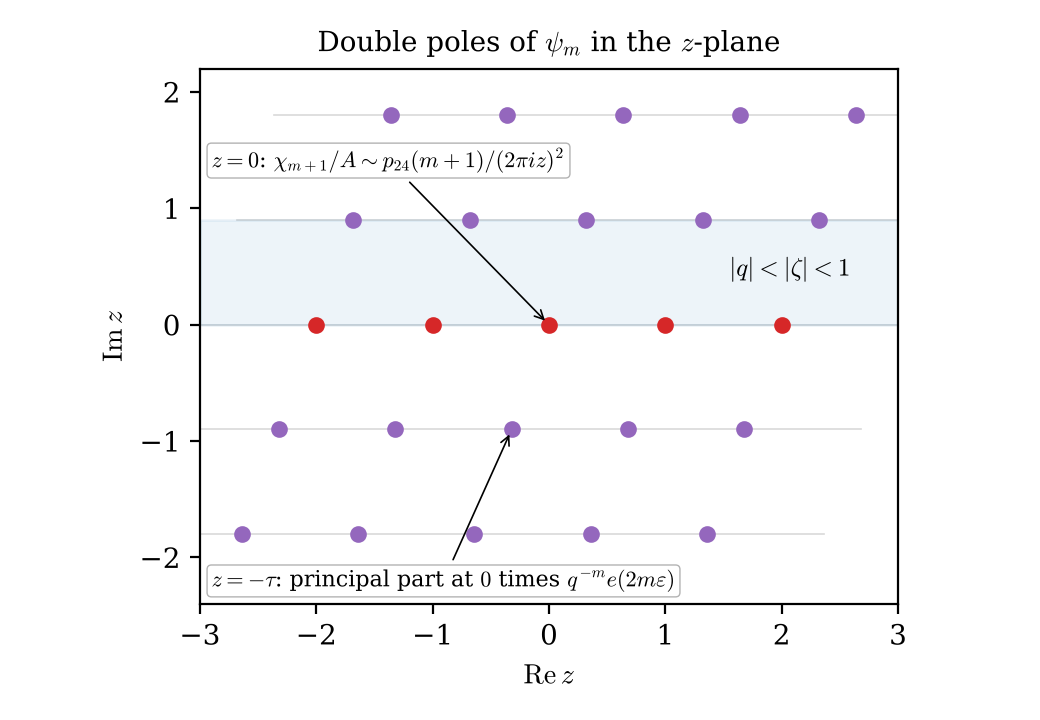
\includegraphics[width=0.72\textwidth]{fig_poles.png}
\caption{The double poles of $\psi_m$ at $z\in\ZZ\tau+\ZZ$, here for $\tau=0.32+0.9i$, and the strip $|q|<|\zeta|<1$ in which $\Delta\psi_m$ and $A_{1,m}$ are expanded. Near $z=0$ the principal part of $\psi_m$ is $\pf(m+1)\Delta^{-1}(2\pi i z)^{-2}$; near $z=-s\tau$ it is the same expression multiplied by $q^{-ms^2}e^{2ms\cdot 2\pi i\varepsilon}$, which produces a simple pole as well. The Appell--Lerch sum $\pf(m+1)A_{1,m}/\Delta$ has exactly these principal parts (Lemma~\ref{lem:poles}).}\label{fig:poles}
\end{figure}

\begin{lemma}\label{lem:Fwell}
For integers $D$ and $r\in\{0,1,\dots,m\}$ with $D\equiv-r^2\pmod{4m}$ put $F_m(D,r)=(-1)^{r+1}\cF_m\bigl((D+r^2)/4m,\,r\bigr)$. Then
\[
(-1)^{l+1}\cF_m(n,l)=F_m(4mn-l^2,r)\qquad\text{for all }n,l,
\]
where $r\in\{0,\dots,m\}$ is the representative of $\pm l$ modulo $2m$, and if the reduced form of a charge $(n,l,m')$ with $D>0$ is $[a,b,c]$, then $\dstar(n,l,m')=F_c(D,b)$. If $m=1$ or $m$ is prime, then $F_m(D,r)$ depends only on $D$, and we write it $F_m(D)$.
\end{lemma}

\begin{proof}
Let $r\equiv\varepsilon l\pmod{2m}$ with $\varepsilon=\pm1$. Then $r^2\equiv l^2\pmod{4m}$, so $(D+r^2)/4m$ is an integer, and $r\equiv l\pmod 2$, so $(-1)^{l+1}=(-1)^{r+1}$. By Lemma~\ref{lem:poles}, $\cF_m(n,l)$ depends only on $4mn-l^2$ and on the class of $\pm l$ modulo $2m$; this gives the first statement. The second is the definition \eqref{eq:dstar}, since $0\le b\le c$.

Let $m=1$ or let $m$ be prime, and let $r,r'\in\{0,\dots,m\}$ with $r^2\equiv r'^2\pmod{4m}$; we show $r=r'$. For $m=1$ the squares $0$ and $1$ are distinct modulo $4$. For prime $m$, $m$ divides $(r-r')(r+r')$. If $m\mid r-r'$, then $r=r'$ or $\{r,r'\}=\{0,m\}$, and the latter is impossible because $m^2\not\equiv0\pmod{4m}$. If $m\mid r+r'$, then $r+r'\in\{0,m,2m\}$. The cases $0$ and $2m$ give $r=r'$. In the case $r+r'=m$ we have $r'^2-r^2=m(m-2r)$, so $4\mid m-2r$; this is impossible for odd $m$, and for $m=2$ the only possibility with $r\ne r'$ is $\{r,r'\}=\{0,2\}$, where $r'^2-r^2=\pm4\not\equiv0\pmod 8$. Hence $r$ is determined by $D$.
\end{proof}

For prime powers $m=p^k$ with $k\ge2$ the value does depend on $r$; for instance, for $m=4$ the residues $r=0$ and $r=4$ both give $D\equiv0\pmod{16}$, and at $D=16$ one finds $F_4(16,0)=-\cF_4(1,0)=185\,738\,352$ but $F_4(16,4)=-\cF_4(2,4)=32\,861\,184$.

\begin{lemma}\label{lem:polar}
The coefficient of $q^{-1}$ in $\psi^F_m$ is the Laurent polynomial
\[
\bigl(\chi^{(0)}_{m+1}(\zeta)-\pf(m+1)\bigr)\frac{\zeta}{(1-\zeta)^2},
\]
which has degree $m$ and leading coefficient $m+2$. In particular $\cF_m(-1,\pm m)=m+2$ and $\cF_m(-1,l)=0$ for $|l|>m$.
\end{lemma}

\begin{proof}
In the strip, the coefficient of $q^{-1}$ in $\psi_m=\Delta^{-1}\chi_{m+1}/A$ is the coefficient of $q^0$ in $\chi_{m+1}/A$, which is $\chi^{(0)}_{m+1}(\zeta)\,\zeta(1-\zeta)^{-2}$. In the expansion of $A_{1,m}$ above, the exponent $n$ vanishes only for $s=0$, where the terms are $(k+1)\zeta^{k+1}$; so the coefficient of $q^0$ in $A_{1,m}$ is $\zeta(1-\zeta)^{-2}$. This proves the formula, since $\chi^{(0)}_{m+1}(1)=\chi_{m+1}(\tau,0)|_{q^0}=\pf(m+1)$ by Lemma~\ref{lem:chi}(i). The numerator vanishes at $\zeta=1$, and so does its derivative because it is invariant under $\zeta\mapsto\zeta^{-1}$; hence it is divisible by $(1-\zeta)^2$ and the quotient is a Laurent polynomial. By Lemma~\ref{lem:chi}(ii) the numerator has degree $m+1$ with leading coefficient $m+2$, the factor $\zeta$ raises the degree by one, and division by $(1-\zeta)^2=\zeta^2(1-\zeta^{-1})^2$ lowers it by two.
\end{proof}


\section{The completion and the class number term}\label{sec:completion}

This section proves Theorem~\ref{thm:D}. The idea is that $A_{1,m}$ and $\mathcal G_m$ are both holomorphic parts of real-analytic functions that transform like Jacobi forms of weight $2$ and index $m$, and that their nonholomorphic parts are proportional. We use the error function in the normalisation of Zwegers,
\[
E(x)=2\int_0^x e^{-\pi t^2}\,dt=\operatorname{erf}(\sqrt\pi\,x),
\]
and the function
\begin{equation}\label{eq:Ifun}
I(x)=\int_1^\infty u^{-3/2}e^{-xu}\,du=2e^{-x}-2\sqrt{\pi x}\,\erfc\sqrt x\qquad(x\ge0),
\end{equation}
where the second expression follows by integrating by parts once and substituting $t=xu$ in $\int_1^\infty u^{-1/2}e^{-xu}du=x^{-1/2}\int_x^\infty t^{-1/2}e^{-t}dt=\sqrt{\pi/x}\,\erfc\sqrt x$. For $m\ge1$ and $l\in\ZZ/2m\ZZ$ put
\begin{equation}\label{eq:Sml}
S_{m,l}(\tau)=y^{-1/2}\sum_{\lambda\equiv l\ (2m)}I\Bigl(\frac{\pi\lambda^2y}{m}\Bigr)q^{-\lambda^2/4m}.
\end{equation}
Since $0<I(x)\le 2e^{-x}$ and $|q^{-\lambda^2/4m}|=e^{\pi\lambda^2y/2m}$, the terms are bounded by $2y^{-1/2}e^{-\pi\lambda^2y/2m}$ and the series converges absolutely and locally uniformly in $\tau$.

\subsection{Zwegers' building block}
For $u\in\CC$ Zwegers defines \cite[Def.~3.2]{Zwe02}
\[
f_u(z;\tau)=\sum_{\lambda\in\ZZ}\frac{q^{m\lambda^2}\zeta^{2m\lambda}}{1-q^\lambda\zeta\,\e(-u)},
\]
a meromorphic function of $z$ with simple poles at $u+\ZZ\tau+\ZZ$, and the real-analytic modification \cite[Def.~3.4]{Zwe02}
\[
\tilde f_u(z;\tau)=f_u(z;\tau)-\frac12\sum_{l\bmod 2m}R_{m,l}(u;\tau)\,\vt_{m,l}(\tau,z),
\]
\[
R_{m,l}(u;\tau)=\sum_{\lambda\equiv l\ (2m)}\Bigl\{\operatorname{sgn}\bigl(\lambda+\tfrac12\bigr)-E\Bigl(\bigl(\lambda+2m\tfrac{\operatorname{Im}u}{y}\bigr)\sqrt{y/m}\Bigr)\Bigr\}\,\e\Bigl(-\frac{\lambda^2\tau}{4m}-\lambda u\Bigr).
\]
For $u$ in a compact set and $|\lambda|$ large the bracket is bounded by $2\exp(-\pi(\lambda+2m\operatorname{Im}u/y)^2y/m)$, because $1-E(x)=\erfc(\sqrt\pi x)\le e^{-\pi x^2}$ for $x\ge0$, while the exponential factor has modulus $\exp(\pi\lambda^2y/2m+2\pi\lambda\operatorname{Im}u)$; so the series for $R_{m,l}$ and its termwise derivatives in $u$ converge locally uniformly. Zwegers proves \cite[Prop.~3.5]{Zwe02} that $\tilde f_u$ satisfies (E) in $z$ with index $m$ and that
\begin{equation}\label{eq:zwmod}
\tilde f_{u/(c\tau+d)}\Bigl(\frac{z}{c\tau+d};\frac{a\tau+b}{c\tau+d}\Bigr)=(c\tau+d)\,\e\Bigl(\frac{mc(z^2-u^2)}{c\tau+d}\Bigr)\tilde f_u(z;\tau)
\end{equation}
for all $\bigl(\begin{smallmatrix}a&b\\c&d\end{smallmatrix}\bigr)\in\mathrm{SL}_2(\ZZ)$. Write $\partial_u=\frac12(\partial_{\operatorname{Re}u}-i\partial_{\operatorname{Im}u})$, so that $\partial_u u=1$, $\partial_u\bar u=0$ and $\partial_u\operatorname{Im}u=1/(2i)$.

\begin{lemma}\label{lem:derivs}
For $z\notin\ZZ\tau+\ZZ$,
\[
\partial_uf_u(z;\tau)\big|_{u=0}=-2\pi i\,A_{1,m}(\tau,z),\qquad \partial_uR_{m,l}(u;\tau)\big|_{u=0}=i\sqrt m\,S_{m,l}(\tau).
\]
\end{lemma}

\begin{proof}
With $w=q^\lambda\zeta$ we have $\partial_u(1-w\,\e(-u))^{-1}=-2\pi i\,w\,\e(-u)(1-w\,\e(-u))^{-2}$, which is $-2\pi i\,w(1-w)^{-2}$ at $u=0$. Multiplying by $q^{m\lambda^2}\zeta^{2m\lambda}$ and summing gives the first formula, since $q^{m\lambda^2}\zeta^{2m\lambda}\cdot q^\lambda\zeta=q^{m\lambda^2+\lambda}\zeta^{2m\lambda+1}$.

For the second, differentiate the term of index $\lambda$ at $u=0$ and put $X=\pi\lambda^2y/m$. Since $E'(x)=2e^{-\pi x^2}$, the derivative of the bracket is
\[
-2e^{-\pi\lambda^2y/m}\cdot\frac{2m}{y}\cdot\frac1{2i}\cdot\sqrt{\frac ym}=2i\sqrt{\frac my}\,e^{-X},
\]
and the derivative of the exponential factor is $-2\pi i\lambda$ times that factor. At $u=0$ the bracket equals $\operatorname{sgn}(\lambda+\frac12)-E(\lambda\sqrt{y/m})$, which is $\erfc\sqrt X$ for $\lambda\ge0$ and $-\erfc\sqrt X$ for $\lambda<0$; times $\lambda$ it equals $|\lambda|\erfc\sqrt X$ in both cases. Hence the derivative of the term is
\[
i\Bigl(2\sqrt{\frac my}\,e^{-X}-2\pi|\lambda|\erfc\sqrt X\Bigr)q^{-\lambda^2/4m}=i\sqrt{\frac my}\Bigl(2e^{-X}-2\sqrt{\pi X}\erfc\sqrt X\Bigr)q^{-\lambda^2/4m},
\]
because $\sqrt{y/m}\cdot\pi|\lambda|=\sqrt{\pi X}$. By \eqref{eq:Ifun} this is $i\sqrt m\,y^{-1/2}I(X)q^{-\lambda^2/4m}$, and summing over $\lambda\equiv l\pmod{2m}$ gives $i\sqrt m\,S_{m,l}$.
\end{proof}

\begin{lemma}\label{lem:Ahat}
The function
\[
\Ah_{1,m}(\tau,z)=A_{1,m}(\tau,z)+\frac{\sqrt m}{4\pi}\sum_{l\bmod 2m}S_{m,l}(\tau)\,\vt_{m,l}(\tau,z)
\]
is real-analytic in $\tau$, meromorphic in $z$ with poles only at $\ZZ\tau+\ZZ$, and satisfies \textup{(E)} and \textup{(M)} with weight $2$ and index $m$.
\end{lemma}

\begin{proof}
By Lemma~\ref{lem:derivs} and the definition of $\tilde f_u$,
\[
-\frac1{2\pi i}\,\partial_u\tilde f_u\big|_{u=0}=A_{1,m}+\frac{1}{4\pi i}\sum_{l}i\sqrt m\,S_{m,l}\vt_{m,l}=\Ah_{1,m}.
\]
The law (E) for $\tilde f_u$ in $z$ does not involve $u$, so it passes to $\partial_u\tilde f_u$. For (M), apply $\partial_u$ to \eqref{eq:zwmod} and put $u=0$. The left side is a function of $u/(c\tau+d)$, which is holomorphic in $u$; by the chain rule its derivative is $(c\tau+d)^{-1}$ times the derivative of $\tilde f$ in its first argument, evaluated at $u=0$. On the right side the factor $\e(-mcu^2/(c\tau+d))$ has derivative zero at $u=0$. Hence
\[
(\partial_u\tilde f)\Bigl(\frac{z}{c\tau+d};\frac{a\tau+b}{c\tau+d}\Bigr)=(c\tau+d)^2\,\e\Bigl(\frac{mcz^2}{c\tau+d}\Bigr)(\partial_u\tilde f)(z;\tau)
\]
at $u=0$, which is (M) with $k=2$. The poles of $f_u$ at $z=u+\ZZ\tau+\ZZ$ become double poles at $\ZZ\tau+\ZZ$ after differentiation, and the theta functions are entire.
\end{proof}

\subsection{Zagier's completion of the class numbers}
Let $F(\tau)=\sum_{N\ge0}H(N)q^N$. Zagier proved that
\begin{equation}\label{eq:zagier}
\widehat F(\tau)=F(\tau)+\frac{1}{16\pi\sqrt y}\sum_{f\in\ZZ}I(4\pi f^2y)\,q^{-f^2}
\end{equation}
satisfies $\widehat F(\gamma\tau)=j(\gamma,\tau)^3\,\widehat F(\tau)$ for every $\gamma\in\Gamma_0(4)$, where $j(\gamma,\tau)=\theta(\gamma\tau)/\theta(\tau)$ and $\theta(\tau)=\sum_{n\in\ZZ}q^{n^2}$; that is, $\widehat F$ transforms like $\theta^3$, a modular form of weight $3/2$ on $\Gamma_0(4)$ \cite{Zag75}, \cite[Ch.~2, Thm.~2]{HZ76}. In \cite{HZ76} the nonholomorphic term is written $y^{-1/2}\sum_f\beta(4\pi f^2y)q^{-f^2}$ with $\beta(x)=\frac1{16\pi}\int_1^\infty u^{-3/2}e^{-xu}du=I(x)/16\pi$. The quotient $j(\gamma,\tau)$ is holomorphic, because $\theta$ has no zeros in $\HH$ by the product $\theta(\tau)=\prod_{n\ge1}(1-q^{2n})(1+q^{2n-1})^2$.

We also need the theta function in two variables, $\theta(\sigma,w)=\sum_{n\in\ZZ}\e(n^2\sigma+nw)$, so that $\theta(\sigma)=\theta(\sigma,0)$. It satisfies $\theta(\sigma,w+1)=\theta(\sigma,w)$, $\theta(\sigma,w+\frac12)=\theta(\sigma+\frac12,w)$ (since $\e(n/2)=\e(n^2/2)$), and $\theta(\sigma,w+2\sigma)=\e(-\sigma-w)\,\theta(\sigma,w)$ (replace $n$ by $n-1$). Moreover, with the principal branch of the square root,
\begin{equation}\label{eq:thetagamma}
\theta\Bigl(\frac{\sigma}{4\sigma+1},\frac{w}{4\sigma+1}\Bigr)=(4\sigma+1)^{1/2}\,\e\Bigl(\frac{w^2}{4\sigma+1}\Bigr)\theta(\sigma,w).
\end{equation}
To see this, put $\Theta(t,z)=\sum_n\exp(\pi in^2t+2\pi inz)$, so that $\theta(\sigma,w)=\Theta(2\sigma,w)$. Poisson summation applied to the Gaussian gives Jacobi's formula $\Theta(-1/t,z/t)=(-it)^{1/2}\exp(\pi iz^2/t)\,\Theta(t,z)$ for $t\in\HH$, and clearly $\Theta(t-2,z)=\Theta(t,z)$ and $\Theta(t,-z)=\Theta(t,z)$. Let $t\in\HH$ and $t_2=-1/t-2\in\HH$, so that $-1/t_2=t/(2t+1)$. Applying Jacobi's formula at $t_2$ with $z/t$, then the periodicity, then Jacobi's formula at $t$,
\[
\Theta\Bigl(\frac t{2t+1},\frac{-z}{2t+1}\Bigr)=(-it_2)^{1/2}(-it)^{1/2}\exp\Bigl(\pi iz^2\Bigl(\frac1{t^2t_2}+\frac1t\Bigr)\Bigr)\Theta(t,z).
\]
Here $t^2t_2=-t(2t+1)$, so the exponent is $2\pi iz^2/(2t+1)$; and $-it$, $-it_2$ lie in the right half-plane, so the product of their principal square roots is the principal square root of $(-it_2)(-it)=2t+1$. Evenness in $z$ and $t=2\sigma$, $z=w$ give \eqref{eq:thetagamma}. At $w=0$ it says $j(\gamma_1,\sigma)=(4\sigma+1)^{1/2}$ for $\gamma_1=\bigl(\begin{smallmatrix}1&0\\4&1\end{smallmatrix}\bigr)$.

For $\mu\in\ZZ/2\ZZ$ put $H_\mu(\tau)=\sum_{N\equiv-\mu^2\ (4)}H(N)q^{N/4}$, so that $\Hc=\sum_\mu H_\mu\vt_{1,\mu}$ by \eqref{eq:thetadec}, and
\[
\widehat H_\mu=H_\mu+\frac1{8\pi}S_{1,\mu},\qquad \Hh=\sum_{\mu\bmod 2}\widehat H_\mu\,\vt_{1,\mu}=\Hc+\frac1{8\pi}\sum_{\mu\bmod2}S_{1,\mu}\vt_{1,\mu}.
\]

\begin{lemma}\label{lem:Hhat}
The function $\Hh$ is real-analytic, entire in $z$, and satisfies \textup{(E)} and \textup{(M)} with weight $2$ and index $1$.
\end{lemma}

\begin{proof}
From \eqref{eq:Sml}, $S_{1,\mu}(4\tau)=(4y)^{-1/2}\sum_{\lambda\equiv\mu\,(2)}I(4\pi\lambda^2y)q^{-\lambda^2}$, so
\[
\widehat H_0(4\tau)+\widehat H_1(4\tau)=\sum_{N}H(N)q^N+\frac1{16\pi\sqrt y}\sum_{\lambda\in\ZZ}I(4\pi\lambda^2y)q^{-\lambda^2}=\widehat F(\tau).
\]
The exponents of $q$ in $\widehat H_\mu$ are $N/4$ with $N\equiv-\mu^2\pmod 4$, and $-\lambda^2/4$ with $\lambda\equiv\mu\pmod2$, so $\widehat H_\mu(\tau+1)=\e(-\mu^2/4)\widehat H_\mu(\tau)$. Hence $\widehat H_0(\tau)+\widehat H_1(\tau)=\widehat F(\sigma)$ and $\widehat H_0(\tau)-\widehat H_1(\tau)=\widehat H_0(\tau+2)+\widehat H_1(\tau+2)=\widehat F(\sigma+\frac12)$, where $\sigma=\tau/4$. On the other side $\vt_{1,0}+\vt_{1,1}=\sum_r\e(r^2\tau/4+rz)=\theta(\sigma,z)$ and $\vt_{1,0}-\vt_{1,1}=\theta(\sigma,z+\frac12)=\theta(\sigma+\frac12,z)$. Therefore
\[
\Hh(\tau,z)=\tfrac12\bigl(\widehat F(\sigma)\,\theta(\sigma,z)+\widehat F(\sigma')\,\theta(\sigma',z)\bigr),\qquad \sigma'=\sigma+\tfrac12 .
\]
The law (E) holds for every function $\sum_\mu h_\mu(\tau)\vt_{1,\mu}(\tau,z)$, since each $\vt_{1,\mu}$ satisfies it. For (M), the matrices $T=\bigl(\begin{smallmatrix}1&1\\0&1\end{smallmatrix}\bigr)$ and $U=\bigl(\begin{smallmatrix}1&0\\1&1\end{smallmatrix}\bigr)$ generate $\mathrm{SL}_2(\ZZ)$, because $T^{-1}UT^{-1}=\bigl(\begin{smallmatrix}0&-1\\1&0\end{smallmatrix}\bigr)$, and the factor in (M) is a cocycle, so it suffices to check (M) for $T$ and $U$. For $T$ it holds because $\widehat H_\mu(\tau+1)\vt_{1,\mu}(\tau+1,z)=\widehat H_\mu(\tau)\vt_{1,\mu}(\tau,z)$. For $U$, which sends $(\tau,z)$ to $(\tau/(\tau+1),z/(\tau+1))$, note that $\sigma$ goes to $\gamma_1\sigma$ and $\tau+1=4\sigma+1$. By \eqref{eq:thetagamma} and the law of $\widehat F$,
\[
\widehat F(\gamma_1\sigma)\,\theta\Bigl(\gamma_1\sigma,\frac z{4\sigma+1}\Bigr)=(4\sigma+1)^{2}\,\e\Bigl(\frac{z^2}{4\sigma+1}\Bigr)\widehat F(\sigma)\,\theta(\sigma,z).
\]
For the second term, $\gamma_1\sigma+\frac12=(3\sigma+\frac12)/(4\sigma+1)=\gamma_2\sigma'$ with $\gamma_2=\bigl(\begin{smallmatrix}3&-1\\4&-1\end{smallmatrix}\bigr)\in\Gamma_0(4)$, whose lower row gives $4\sigma'-1=4\sigma+1$. Writing $\frac12=(2\sigma+\frac12)/(4\sigma+1)$ and applying \eqref{eq:thetagamma} with $w=z+2\sigma+\frac12$, then the quasi-periodicity,
\[
\theta\Bigl(\gamma_2\sigma',\frac z{4\sigma+1}\Bigr)=\theta\Bigl(\gamma_1\sigma,\frac{z+2\sigma+\frac12}{4\sigma+1}\Bigr)=(4\sigma+1)^{1/2}\,\e\Bigl(\frac{(z+2\sigma+\frac12)^2}{4\sigma+1}-\sigma-z-\frac12\Bigr)\theta(\sigma',z),
\]
and the exponent equals $z^2/(4\sigma+1)-\frac14$, as one checks by expanding $(z+2\sigma+\frac12)^2-(\sigma+z+\frac12)(4\sigma+1)=z^2-\sigma-\frac14$. At $z=0$ this gives $j(\gamma_2,\sigma')=-i(4\sigma+1)^{1/2}$. Hence
\[
\widehat F(\gamma_2\sigma')\,\theta\Bigl(\gamma_2\sigma',\frac z{4\sigma+1}\Bigr)=(-i)^4(4\sigma+1)^{2}\,\e\Bigl(\frac{z^2}{4\sigma+1}\Bigr)\widehat F(\sigma')\,\theta(\sigma',z).
\]
Adding the two identities gives $\Hh(U(\tau,z))=(\tau+1)^2\e(z^2/(\tau+1))\Hh(\tau,z)$, which is (M) for $U$ with $k=2$ and $m=1$. Real-analyticity is clear from the definition, and $\Hh$ is entire in $z$ because the theta functions are.
\end{proof}

For a positive integer $k$ and integers $\Lambda,R$ with $R\equiv\Lambda\pmod2$ put $t=(R-\Lambda)/2$ and $u=(R+\Lambda)/2$, so that $tu=(R^2-\Lambda^2)/4$, and let
\[
N_k(\Lambda,R)=\#\bigl\{(a,d):\ ad=k,\ a\mid t,\ a\mid u,\ d\mid tu/a^2\bigr\};
\]
put $N_k(\Lambda,R)=0$ if $R\not\equiv\Lambda\pmod 2$. For $m\ge1$ let $T_m(\Lambda,R)=[\Lambda\equiv R\ (2m)]+[\Lambda\equiv-R\ (2m)]$, where $[\cdot]$ is $1$ if the condition holds and $0$ otherwise. For a function $\Phi$ of the form $\frac{1}{8\pi\sqrt y}\sum_{\Lambda,R}w(\Lambda,R)\,I(\pi\Lambda^2y/k)\,\e\bigl((R^2-\Lambda^2)\tau/4k\bigr)\zeta^R$ we say that $\Phi$ has index $k$ and \emph{weight} $w$. The summand depends on $\Lambda$ only through $\Lambda^2$, so two weights with the same symmetrisation $w(\Lambda,R)+w(-\Lambda,R)$ give the same function.

\begin{lemma}\label{lem:Ahatw}
The nonholomorphic part $\Ah_{1,m}-A_{1,m}$ of Lemma~\ref{lem:Ahat} has index $k=m$ and weight $\sqrt m\,T_m$. The nonholomorphic part $\Hh-\Hc$ of Lemma~\ref{lem:Hhat} has index $k=1$ and weight $N_1$.
\end{lemma}

\begin{proof}
By \eqref{eq:Sml} and the definition of $\vt_{m,l}$,
\[
\frac{\sqrt m}{4\pi}\sum_{l\bmod 2m}S_{m,l}\vt_{m,l}=\frac{\sqrt m}{4\pi\sqrt y}\sum_{\Lambda\equiv R\ (2m)}I\Bigl(\frac{\pi\Lambda^2y}{m}\Bigr)\e\Bigl(\frac{(R^2-\Lambda^2)\tau}{4m}\Bigr)\zeta^R .
\]
The substitution $\Lambda\mapsto-\Lambda$ shows that the sum over $\Lambda\equiv R$ equals the sum over $\Lambda\equiv-R$, so twice it is the sum with weight $T_m$; this gives the first statement. For $m=1$ the condition $\Lambda\equiv R\pmod2$ is $N_1(\Lambda,R)=1$, and $\Hh-\Hc=\frac1{8\pi}\sum_\mu S_{1,\mu}\vt_{1,\mu}$ is the same sum with $\frac1{8\pi}$ in place of $\frac1{4\pi}$.
\end{proof}

\begin{lemma}\label{lem:Vk}
Let $k\ge1$. Then $\Hh|_2V_k-\Hc|V_k$ has index $k$ and weight $\sqrt k\,N_k$, where $\Hc|V_k$ has the coefficients \eqref{eq:HVm}.
\end{lemma}

\begin{proof}
The operator $V_k$ is linear and is applied termwise to absolutely convergent series; on $\Hc$ it gives \eqref{eq:HVm} by \eqref{eq:heckecoef}. It remains to compute $G|_2V_k$ for
\[
G(\tau,z)=\Hh-\Hc=\frac{1}{8\pi\sqrt y}\sum_{\lambda\in\ZZ}\ \sum_{r\equiv\lambda\,(2)}I(\pi\lambda^2y)\,\e\Bigl(\frac{(r^2-\lambda^2)\tau}{4}\Bigr)\zeta^r .
\]
By definition $G|_2V_k=k\sum_{ad=k}\sum_{b\bmod d}d^{-2}G\bigl(\frac{a\tau+b}{d},az\bigr)$. In the term belonging to $(a,d,b)$ the imaginary part $y$ is replaced by $ay/d$, the exponential factor acquires $\e(b(r^2-\lambda^2)/4d)$, and $\zeta^r$ becomes $\zeta^{ar}$. Summing over $b\bmod d$ gives $d$ if $d$ divides the integer $(r^2-\lambda^2)/4$ and $0$ otherwise. So the contribution of the pair $(a,d)$ is
\[
\frac{k}{d}\sqrt{\frac da}\,\frac{1}{8\pi\sqrt y}\sum_{\substack{r\equiv\lambda\,(2)\\ d\,\mid\,(r^2-\lambda^2)/4}}I\Bigl(\frac{\pi\lambda^2ay}{d}\Bigr)\e\Bigl(\frac{a(r^2-\lambda^2)\tau}{4d}\Bigr)\zeta^{ar}.
\]
Put $\Lambda=a\lambda$ and $R=ar$. Then $\pi\lambda^2ay/d=\pi\Lambda^2y/k$, $a(r^2-\lambda^2)/4d=(R^2-\Lambda^2)/4k$, and $\frac kd\sqrt{d/a}=\sqrt k$. The pairs $(\Lambda,R)$ that occur are those with $a\mid\Lambda$, $a\mid R$ and $\Lambda/a\equiv R/a\pmod2$, that is, with $a\mid t$ and $a\mid u$; and the condition on $d$ reads $d\mid tu/a^2$. Summing over $(a,d)$ gives the weight $\sqrt k\,N_k$. All series converge absolutely and locally uniformly, since $N_k\le k$, $I(x)\le2e^{-x}$ and $|\e((R^2-\Lambda^2)\tau/4k)|=e^{-\pi(R^2-\Lambda^2)y/2k}$, so the terms are bounded by $2k\,e^{-\pi(R^2+\Lambda^2)y/2k}|\zeta|^R$.
\end{proof}

For an integer $e\ge1$ and a function $\Phi$ satisfying (E) and (M) with weight $2$ and index $j$, the function $\Phi|U_e(\tau,z)=\Phi(\tau,ez)$ satisfies (E) and (M) with weight $2$ and index $je^2$: in (M) the factor $\e(jc(ez)^2/(c\tau+d))$ becomes $\e(je^2cz^2/(c\tau+d))$, and in (E) the shift $z\mapsto z+\lambda\tau+\mu$ becomes $ez\mapsto ez+e\lambda\tau+e\mu$. If $\Phi$ has index $j$ and weight $w$ in the sense above, then $\Phi|U_e$ has index $je^2$ and weight $(\Lambda,R)\mapsto[e\mid\Lambda,\,e\mid R]\,w(\Lambda/e,R/e)$: replacing $\zeta$ by $\zeta^e$ and writing $\Lambda'=e\Lambda$, $R'=eR$ turns $I(\pi\Lambda^2y/j)$ into $I(\pi\Lambda'^2y/je^2)$ and $(R^2-\Lambda^2)/4j$ into $(R'^2-\Lambda'^2)/4je^2$.

\begin{lemma}\label{lem:count}
Let $m=p^k$ be a prime power and let $R\equiv\Lambda\pmod 2$. Then
\[
N_m(\Lambda,R)-[\,p\mid t,\ p\mid u\,]\,N_{m/p^2}(\Lambda/p,R/p)=T_m(\Lambda,R),
\]
where the second term is absent when $k=1$.
\end{lemma}

\begin{proof}
Let $\alpha=v_p(t)$ and $\beta=v_p(u)$, with $v_p(0)=\infty$; by symmetry we may assume $\alpha\le\beta$. A factorisation $m=ad$ is $a=p^j$, $d=p^{k-j}$ with $0\le j\le k$, and the conditions $a\mid t$, $a\mid u$, $d\mid tu/a^2$ read $j\le\alpha$ and $\alpha+\beta\ge k+j$. Hence
\[
N_m(\Lambda,R)=\#\{\,j:\ 0\le j\le\min(\alpha,k,\alpha+\beta-k)\,\}.
\]
The congruence $\Lambda\equiv R\pmod{2m}$ means $p^k\mid t$, and $\Lambda\equiv-R$ means $p^k\mid u$; so $T_m=[\alpha\ge k]+[\beta\ge k]$. If $p\mid t$ and $p\mid u$, the pair $(\Lambda/p,R/p)$ has $t/p$, $u/p$ in place of $t,u$, with valuations $\alpha-1$, $\beta-1$, and the same description with $k-2$ in place of $k$ and the substitution $j=j'+1$ gives
\[
N_{m/p^2}(\Lambda/p,R/p)=\#\{\,j:\ 1\le j\le\min(\alpha,k-1,\alpha+\beta-k+1)\,\}.
\]
Let $k\ge2$; we go through the four possible cases.

If $\alpha+\beta<k$, the first set is empty, and so is the second because $\alpha+\beta-k+1\le0$; and $T_m=0$ since $\beta\le\alpha+\beta<k$.

If $\alpha+\beta\ge k$ and $\beta<k$, then $\alpha\ge1$ and the subtracted term is present. Here $\alpha+\beta-k<\alpha$ and $\alpha+\beta-k+1\le\min(\alpha,k-1)$, so the two counts are $\alpha+\beta-k+1$ and $\alpha+\beta-k+1$, and their difference is $0=T_m$.

If $\alpha<k\le\beta$, the first count is $\alpha+1$. If $\alpha=0$ the subtracted term is absent and the difference is $1$. If $\alpha\ge1$ the second count is $\alpha$, since $\alpha\le k-1$ and $\alpha+\beta-k+1\ge\alpha+1$; the difference is again $1$. In both cases $T_m=1$.

If $\alpha\ge k$, then $\beta\ge k$, the counts are $k+1$ and $k-1$, and the difference is $2=T_m$.

For $k=1$ the first set is $\{j\in\{0,1\}:j\le\alpha,\ \alpha+\beta\ge1+j\}$, which has $0$, $1$ or $2$ elements according as $\beta=0$, $\alpha=0<\beta$ or $\alpha\ge1$; this is $[\alpha\ge1]+[\beta\ge1]$.
\end{proof}

\subsection{Proof of Theorem~\ref{thm:D}}
Let $m=1$ or let $m=p^k$ be a prime power, and put $\widehat{\mathcal G}_1=\Hh$, $\widehat{\mathcal G}_p=\Hh|V_p$ and $\widehat{\mathcal G}_{p^k}=\Hh|V_{p^k}-p\,(\Hh|V_{p^{k-2}})|U_p$ for $k\ge2$. By Lemma~\ref{lem:Hhat}, \cite[Thm.~4.2]{EZ85} and the remark on $U_e$, $\widehat{\mathcal G}_m$ satisfies (E) and (M) with weight $2$ and index $m$, and its holomorphic part is $\mathcal G_m$; by Lemma~\ref{lem:Vk} and the rule for $U_p$, its nonholomorphic part $\widehat{\mathcal G}_m-\mathcal G_m$ has index $m$ and weight
\begin{align*}
&\sqrt m\,N_m(\Lambda,R)-p\sqrt{m/p^2}\,[p\mid\Lambda,\,p\mid R]\,N_{m/p^2}(\Lambda/p,R/p)\\
&\qquad=\sqrt m\bigl(N_m(\Lambda,R)-[p\mid t,\,p\mid u]\,N_{m/p^2}(\Lambda/p,R/p)\bigr)
\end{align*}
for $k\ge2$, and $\sqrt m\,N_m$ for $k\le1$. In the second expression we used that $N_{m/p^2}(\Lambda/p,R/p)=0$ unless $\Lambda/p\equiv R/p\pmod 2$, and under $p\mid\Lambda$, $p\mid R$ this congruence is equivalent to $p\mid t$ and $p\mid u$. By Lemma~\ref{lem:count} the weight is $\sqrt m\,T_m$ when $m$ is a prime power. For $m=1$ it is $N_1$, and $T_1=2N_1$ because $\Lambda\equiv R$ and $\Lambda\equiv-R$ are the same condition modulo $2$. Comparing with Lemma~\ref{lem:Ahatw}, $\widehat{\mathcal G}_m-\mathcal G_m=\kappa_m(\Ah_{1,m}-A_{1,m})$ with $\kappa_1=\frac12$ and $\kappa_m=1$ for prime powers, that is, $\lambda_m\kappa_m=\pf(m+1)$.

By \eqref{eq:psiF},
\[
\phi_m=\Delta\psi^F_m+\lambda_m\mathcal G_m=\frac{\chi_{m+1}}{A}-\pf(m+1)A_{1,m}+\lambda_m\mathcal G_m=\frac{\chi_{m+1}}{A}-\pf(m+1)\Ah_{1,m}+\lambda_m\widehat{\mathcal G}_m,
\]
and each of the three terms on the right satisfies (E) and (M) with weight $2$ and index $m$: the first because $\chi_{m+1}$ and $A$ are weak Jacobi forms of weights $0,-2$ and indices $m+1,1$, the second by Lemma~\ref{lem:Ahat}, and the third as just shown. On the other hand $\phi_m$ is holomorphic in $\tau$ and in $z$, because $\psi^F_m$ is (Lemma~\ref{lem:poles}) and $\mathcal G_m$ is a theta series with polynomially bounded coefficients ($H(N)\le N+1$ by Lemma~\ref{lem:hurwitz}). Its expansion has $n\ge0$, since $\psi^F_m$ has $n\ge-1$ and $\mathcal G_m$ has $n\ge0$. So $\phi_m$ is a weak Jacobi form of weight $2$ and index $m$.

For the explicit form, \eqref{eq:ring} gives $\phi_m=\sum_i x_iM_i$ for the monomials $M_i=E_4^\alpha E_6^\beta A^i(2\phi_{0,1})^{m-i}$ with $4\alpha+6\beta-2i=2$, $1\le i\le m$; there are $1,2,3,6,9,18,23$ of them for $m=1,2,3,5,7,11,13$. The identity $\Delta\psi^F_m=\sum_ix_iM_i-\lambda\,\mathcal G_m$ is linear in the unknowns $(x_i,\lambda)$. We computed the coefficients of $q^n\zeta^l$, $0\le n\le14$, $0\le l\le m$, of $\Delta\psi^F_m$, of the $M_i$ and of $\mathcal G_m$ in exact rational arithmetic (Appendix~\ref{app:computation}), and found that the resulting matrix has full column rank and that the system has the solution listed in Appendix~\ref{app:data}, with $\lambda=\lambda_m$. Since a solution exists by the first part of the proof and the rank is full, the solution is unique, and the $x_i$ are the coefficients of $\phi_m$. The same computation for $m=4,8,9$ confirms the first part: the system with $\mathcal G_m$ is consistent of full rank with $\lambda=\lambda_m$, while for $m=4$ the system with $\Hc|V_4$ in place of $\mathcal G_4$ has no solution. \qed

\begin{remark}\label{rem:composite}
When $m$ has two distinct prime factors the count of Lemma~\ref{lem:count} fails. For $m=6$ the only function $\Hc|V_{6/e^2}|U_e$ of index $6$ is $\Hc|V_6$, and its weight $N_6$ is not a multiple of $T_6$: at $\Lambda=1$ one has $N_6(1,1)=N_6(1,5)=1$, while $T_6(1,1)=1$ and $T_6(1,5)=0$; at $(\Lambda,R)=(0,0)$, $N_6=4$ and $T_6=2$. Correspondingly, the linear system above for $m=6$, with $\Hc|V_6$ and the coefficients $0\le n\le12$, has no solution. Another mock modular correction is needed for such $m$, and we have not determined it. This is why Theorem~\ref{thm:B} is restricted to $m=1$ and prime powers.
\end{remark}

\section{The exact formula}\label{sec:rademacher}

Let $m\in\Mset$. By Theorem~\ref{thm:D}, $\phi_m/\Delta$ is a weakly holomorphic Jacobi form of weight $-10$ and index $m$. We write its coefficients as $a_m(n,l)$, and, since they depend only on $D=4mn-l^2$ and on $l\bmod 2m$, also as $a_m(D,l)$. Let $\delta_m(n,l)$ be the coefficient of $q^n\zeta^l$ in $\mathcal G_m/\Delta$, so that
\begin{equation}\label{eq:hdelta}
\delta_m(n,l)=\sum_{j\ge0}\pf(j)\,g_m(n+1-j,l),\qquad \cF_m(n,l)=a_m(n,l)-\lambda_m\,\delta_m(n,l),
\end{equation}
with $g_m$ as in \eqref{eq:Gm}. The pairs $(D',l')$ with $D'<0$ and $a_m(D',l')\ne0$ are the \emph{polar terms}; there are finitely many classes of them, because $a_m(n,l)=0$ for $n<-1$ and the coefficients of a weak Jacobi form vanish for $4mn-l^2<-m^2$. The most polar one is $D'=-m(m+4)$, $l'\equiv m$, where $a_m=\cF_m(-1,m)=m+2$ by Lemma~\ref{lem:polar}, since $g_m(0,m)=0$. Because $g_m(k,l)=0$ when $4mk-l^2<0$, the term of index $j$ in $\delta_m(n,l)$ vanishes unless $4mn-l^2\ge-4m(1-j)$; so $\delta_m$ vanishes at discriminants below $-4m$, and the polar coefficients of $\phi_m/\Delta$ and of $\psi^F_m$ agree for $D'<-4m$ and differ by $\lambda_m\delta_m(D',l')$ for $-4m\le D'<0$. All polar coefficients $a_m(D',l')$ are listed in Appendix~\ref{app:data}.

By \eqref{eq:thetadec} and \eqref{eq:hmod}, the functions $g_l(\tau)=\sum_Da_m(D,l)q^{D/4m}$, $l\in\ZZ/2m\ZZ$, form a vector-valued weakly holomorphic modular form of weight $w=-\frac{21}2$ for $\mathrm{SL}_2(\ZZ)$ (more precisely for its metaplectic double cover), with a representation $\rho$ determined by \eqref{eq:hmod}. The matrices in \eqref{eq:hmod} are unitary: the first is diagonal with entries of modulus one, and the second is a scalar of modulus one times $(2m)^{-1/2}(\e(lj/2m))_{l,j}$, whose rows are orthonormal. Hence $\rho$ is unitary. Put $\nu=1-w=\frac{23}2$. Exact formulae of the following kind for the coefficients of modular forms of negative weight go back to Rademacher and Zuckerman \cite{RZ38}.

\begin{theorem}\label{thm:rademacher}
For $D>0$ with $D\equiv-l^2\pmod{4m}$,
\begin{equation}\label{eq:rademacher}
a_m(D,l)=\sum_{c\ge1}\frac{2\pi}{c}\sum_{(D',l')}a_m(D',l')\,K_c(D',l';D,l)\Bigl(\frac{|D'|}{D}\Bigr)^{\nu/2}I_\nu\Bigl(\frac{\pi\sqrt{|D'|D}}{mc}\Bigr),
\end{equation}
where $(D',l')$ runs over the polar terms with $l'\in\ZZ/2m\ZZ$, $I_\nu$ is the modified Bessel function of the first kind, and the Kloosterman sum $K_c(D',l';D,l)$ is a sum of $\varphi(c)$ complex numbers of modulus at most one. For $c=1$, $K_1(D',l';D,l)=-(2m)^{-1/2}\e(ll'/2m)$. The series converges absolutely.
\end{theorem}

\begin{proof}
For vector-valued modular forms of negative weight with a unitary representation, Bruinier constructs for each polar term a Maass--Poincar\'e series of weight $w$ whose principal part is $q^{D'/4m}(\mathfrak e_{l'}+\mathfrak e_{-l'})$, where $\mathfrak e_l$ is the standard basis vector, and computes its Fourier expansion \cite[Def.~1.8, Prop.~1.10]{Bru02}. Its holomorphic part has, for $D>0$, the coefficients given by the sum over $c$ in \eqref{eq:rademacher}, where $K_c(D',l';D,l)$ is a sum over $d\bmod c$ with $(c,d)=1$ of a root of unity times an entry of $\rho(\gamma)^{-1}$, for a matrix $\gamma\in\mathrm{SL}_2(\ZZ)$ with lower row $(c,d)$ \cite[Prop.~1.10]{Bru02}; Manschot and Moore give the same series in the notation of Jacobi forms \cite[\S\S2--3]{MM10}. Since $\rho$ is unitary, each term of $K_c$ has modulus at most one. For $c=1$ there is one term, with $\gamma=S=\bigl(\begin{smallmatrix}0&-1\\1&0\end{smallmatrix}\bigr)$, and the entry of $\rho(S)$ given by \eqref{eq:hmod} with $k=-10$ yields $K_1=-(2m)^{-1/2}\e(\pm ll'/2m)$; the sign of the exponent is immaterial because $a_m(D',l')=a_m(D',-l')$ and the sum in \eqref{eq:rademacher} contains both $l'$ and $-l'$.

Let $P$ be the sum over the polar terms of $a_m(D',l')$ times the corresponding Poincar\'e series (each pair $\pm l'$ taken once). Then $h=(g_l)_l-P$ transforms with weight $w$ and representation $\rho$, is annihilated by the weight $w$ Laplacian, and has no principal part. Its image $\xi_w(h)$ under the antilinear operator $\xi_w=2iy^w\overline{\partial_{\bar\tau}}$ is a cusp form of weight $2-w$ for the dual representation \cite[Prop.~3.2]{BF04}. By \cite[Prop.~3.5]{BF04}, the Petersson norm of $\xi_w(h)$ equals a finite sum of products $c_h^+(n)\,b(-n)$ over $n\le0$, where $c_h^+(n)$ are the coefficients of the holomorphic part of $h$ and $b(n)$ those of $\xi_w(h)$. For $n<0$ the first factor vanishes because $h$ has no principal part, and for $n=0$ the second vanishes because $\xi_w(h)$ is a cusp form; so $\xi_w(h)=0$. Hence $h$ is a weakly holomorphic modular form of negative weight without principal part, that is, a holomorphic modular form of negative weight, and therefore $h=0$. So $(g_l)=P$, and comparing holomorphic parts gives \eqref{eq:rademacher}.

Absolute convergence: $I_\nu(t)\le(t/2)^\nu e^t/\Gamma(\nu+1)$ (Lemma~\ref{lem:besselupper}), so the term of index $c$ is $O(c^{-1}\varphi(c)c^{-\nu})=O(c^{-\nu})$ and $\nu>1$.
\end{proof}

As a check on the normalisation, the terms with $c=1$ of \eqref{eq:rademacher} reproduce the exact coefficients $a_m(n,l)$ computed from the definitions to a relative accuracy better than $10^{-48}$ at the largest $n$ in our tables, for every $m\in\Mset$ and $0\le l\le m$ (Appendix~\ref{app:computation}).

\subsection{Main term and error terms}
For $(D',l')$ a polar term with $0\le l'\le m$, put $w_{l'}=1$ if $l'\in\{0,m\}$ and $w_{l'}=2$ otherwise; this is the number of classes $\pm l'$ modulo $2m$. Let
\[
x_{D'}(D)=\frac{\pi\sqrt{|D'|D}}{m},\qquad \alpha=\alpha_m=\pi\sqrt{\frac{m+4}{m}},
\]
so that the most polar term has $x_{-m(m+4)}(D)=\alpha\sqrt D$. The main term is
\begin{equation}\label{eq:mainterm}
T(D)=T_m(D)=\frac{2\pi}{\sqrt{2m}}\,(m+2)\Bigl(\frac{m(m+4)}{D}\Bigr)^{\nu/2}I_\nu(\alpha\sqrt D).
\end{equation}
The terms with $c=1$ of \eqref{eq:rademacher} are
\[
-\frac{2\pi}{\sqrt{2m}}\sum_{(D',l')}w_{l'}\,a_m(D',l')\cos\Bigl(\frac{\pi ll'}{m}\Bigr)\Bigl(\frac{|D'|}{D}\Bigr)^{\nu/2}I_\nu\bigl(x_{D'}(D)\bigr),
\]
now with $0\le l'\le m$. For the most polar term, $\cos(\pi lm/m)=(-1)^l$, so its contribution to $F_m(D,l)=(-1)^{l+1}\cF_m(n,l)$, $0\le l\le m$, is exactly $T(D)$, whatever the class $l$.

\begin{proposition}\label{prop:decomp}
Let $m\in\Mset$, let $0\le l\le m$, let $D\ge4m$ with $D\equiv-l^2\pmod{4m}$, and let $\mathcal S$ be any set of polar terms. Then
\[
|F_m(D,l)-T(D)|\le E_1(D)+E_2(D)+E_3(D),
\]
where, with $B_1(t)=e^t/\sqrt{2\pi t}$, $B_2(t)=(t/2)^\nu e^t/\Gamma(\nu+1)$ and $Z=\sum_{c\ge2}c^{-\nu}$,
\begin{align*}
E_1(D)&=\frac{2\pi}{\sqrt{2m}}\sum_{(D',l')\ne(-m(m+4),m)}w_{l'}|a_m(D',l')|\Bigl(\frac{|D'|}{D}\Bigr)^{\nu/2}B_{(D',l')}\bigl(x_{D'}(D)\bigr),\\
E_2(D)&=\frac{2\pi Z}{\Gamma(\nu+1)}\sum_{(D',l')}w_{l'}|a_m(D',l')|\Bigl(\frac{|D'|}{D}\Bigr)^{\nu/2}\Bigl(\frac{x_{D'}(D)}2\Bigr)^{\nu}e^{x_{D'}(D)/2},\\
E_3(D)&=\lambda_m\,\sigma^*(m)\,(D+4m+1)\Bigl(25+c_0\Bigl(\frac{D}{4m}\Bigr)^{-5}e^{2\pi\sqrt{D/m}}\Bigr),
\end{align*}
$B_{(D',l')}=B_2$ for $(D',l')\in\mathcal S$ and $B_1$ otherwise, $\sigma(m)$ is the sum of the divisors of $m$, $\sigma^*(m)=\sigma(m)$ for $m=1$ or $m$ prime, $\sigma^*(p^k)=\sigma(p^k)+p\,\sigma(p^{k-2})$ for $k\ge2$, and $c_0=\prod_{k\ge1}(1-e^{-2\pi k})^{-24}<1.046$.
\end{proposition}

\begin{proof}
By \eqref{eq:hdelta}, $F_m(D,l)=(-1)^{l+1}a_m(D,l)-(-1)^{l+1}\lambda_m\delta_m(n,l)$. In \eqref{eq:rademacher}, the terms with $c=1$ other than the main term are bounded in absolute value by $E_1(D)$, because $|\cos|\le1$ and $I_\nu\le B_1$, $I_\nu\le B_2$ (Lemma~\ref{lem:besselupper}). For $c\ge2$ we have $c^{-1}|K_c|\le c^{-1}\varphi(c)\le1$, and by the series of $I_\nu$, $I_\nu(t/c)\le(t/2c)^\nu e^{t/c}/\Gamma(\nu+1)\le c^{-\nu}(t/2)^\nu e^{t/2}/\Gamma(\nu+1)$; summing over $c\ge2$ and over the classes gives $E_2(D)$. The bound $\lambda_m|\delta_m(n,l)|\le E_3(D)$ is Lemma~\ref{lem:deltabound}.
\end{proof}

\begin{lemma}\label{lem:deltabound}
For $D=4mn-l^2\ge4m$ and $m\in\Mset$, $|\delta_m(n,l)|\le\sigma^*(m)(D+4m+1)\bigl(25+c_0(D/4m)^{-5}e^{2\pi\sqrt{D/m}}\bigr)$.
\end{lemma}

\begin{proof}
The term $j$ of \eqref{eq:hdelta} involves $g_m(k,l)$ with $k=n+1-j$, whose discriminant is $N=4mk-l^2=D+4m(1-j)$. It vanishes unless $N\ge0$, that is unless $j\le J$ with $J=1+D/4m$. For such $j$, \eqref{eq:HVm} and Lemma~\ref{lem:hurwitz} give $|h_m(k,l)|\le\sum_{d\mid m}d\,(N+1)\le\sigma(m)(D+4m+1)$, and for $m=p^k$, $k\ge2$, the second term of $g_m(k,l)$ is $p\,h_{m/p^2}(k,l/p)$, whose argument has discriminant $N/p^2$, so it is at most $p\,\sigma(p^{k-2})(D+4m+1)$. Hence $|g_m(k,l)|\le\sigma^*(m)(D+4m+1)$ and
\[
|\delta_m(n,l)|\le\sigma^*(m)(D+4m+1)\sum_{0\le j\le J}\pf(j).
\]
Here $\pf(0)+\pf(1)=25$, and for $2\le j\le J$ Lemma~\ref{lem:partitions} gives $\pf(j)\le c_0\,t^{-6}e^{4\pi\sqrt t}$ with $t=j-1\in[1,J-1]$. The function $t^{-6}e^{4\pi\sqrt t}$ is increasing for $t\ge1$, since its logarithmic derivative $-6/t+2\pi/\sqrt t$ is positive for $t>9/\pi^2$. There are at most $J-1$ such $j$, so their sum is at most $(J-1)c_0(J-1)^{-6}e^{4\pi\sqrt{J-1}}$, and $J-1=D/4m\ge1$, $4\pi\sqrt{D/4m}=2\pi\sqrt{D/m}$.
\end{proof}

\section{Bessel functions}\label{sec:bessel}

We use the integral representation \cite[\S3.71]{Wat44}
\begin{equation}\label{eq:poisson}
I_\nu(x)=\frac{(x/2)^\nu}{\sqrt\pi\,\Gamma(\nu+\frac12)}\int_{-1}^1(1-t^2)^{\nu-\frac12}e^{xt}\,dt\qquad(\nu>-\tfrac12,\ x>0),
\end{equation}
the series $I_\nu(x)=\sum_{k\ge0}(x/2)^{\nu+2k}/(k!\,\Gamma(\nu+k+1))$, and the recurrences $I_\nu'=I_{\nu+1}+\frac\nu xI_\nu$, $I_{\nu+1}'=I_\nu-\frac{\nu+1}xI_{\nu+1}$ \cite[\S3.71]{Wat44}. Substituting $t=1-u$ in \eqref{eq:poisson} gives
\begin{equation}\label{eq:poisson2}
I_\nu(x)=\frac{(x/2)^\nu e^x}{\sqrt\pi\,\Gamma(\nu+\frac12)}\int_0^2u^{\nu-\frac12}(2-u)^{\nu-\frac12}e^{-xu}\,du .
\end{equation}

\begin{lemma}\label{lem:besselupper}
For $\nu\ge\frac12$ and $x>0$, $I_\nu(x)\le e^x/\sqrt{2\pi x}$. For $\nu\ge0$ and $x>0$, $I_\nu(x)\le(x/2)^\nu e^x/\Gamma(\nu+1)$.
\end{lemma}

\begin{proof}
For $\nu\ge\frac12$, bound $(2-u)^{\nu-\frac12}\le2^{\nu-\frac12}$ in \eqref{eq:poisson2} and extend the integral to $(0,\infty)$:
\[
I_\nu(x)\le\frac{(x/2)^\nu e^x}{\sqrt\pi\,\Gamma(\nu+\frac12)}\,2^{\nu-\frac12}\,\Gamma(\nu+\tfrac12)\,x^{-\nu-\frac12}=\frac{e^x}{\sqrt{2\pi x}}.
\]
For the second bound, $\Gamma(\nu+k+1)=\Gamma(\nu+1)(\nu+1)\cdots(\nu+k)\ge\Gamma(\nu+1)\,k!$, so
\[
I_\nu(x)\le\frac{(x/2)^\nu}{\Gamma(\nu+1)}\sum_{k\ge0}\frac{(x/2)^{2k}}{k!^2}=\frac{(x/2)^\nu}{\Gamma(\nu+1)}\,I_0(x),
\]
and $I_0(x)=\frac1\pi\int_{-1}^1(1-t^2)^{-1/2}e^{xt}dt\le e^x$ by \eqref{eq:poisson} with $\nu=0$.
\end{proof}

\begin{lemma}\label{lem:besselower}
Let $\nu=\frac{23}2$ and $0<s<2$. For $x>0$,
\[
I_\nu(x)\ge\frac{e^x}{\sqrt{2\pi x}}\,\Bigl(1-\frac s2\Bigr)^{11}P(12,sx),\qquad P(12,t)=\frac{1}{11!}\int_0^tv^{11}e^{-v}\,dv .
\]
\end{lemma}

\begin{proof}
In \eqref{eq:poisson2}, $\nu-\frac12=11$. Keep only $0\le u\le s$, where $2-u\ge2(1-s/2)$:
\[
\int_0^2u^{11}(2-u)^{11}e^{-xu}du\ge2^{11}\Bigl(1-\frac s2\Bigr)^{11}\int_0^su^{11}e^{-xu}du=2^{11}\Bigl(1-\frac s2\Bigr)^{11}x^{-12}\,11!\,P(12,sx).
\]
Since $\Gamma(\nu+\frac12)=11!$, this gives $I_\nu(x)\ge(x/2)^{23/2}e^x\pi^{-1/2}2^{11}x^{-12}(1-s/2)^{11}P(12,sx)$, and $(x/2)^{23/2}2^{11}x^{-12}\pi^{-1/2}=(2\pi x)^{-1/2}$.
\end{proof}

We use $s=\frac15$. The factor $\kappa(x)=(1-\frac s2)^{11}P(12,sx)$ is increasing in $x$ and tends to $0.9^{11}=0.3138\ldots$ as $x\to\infty$.

\begin{lemma}\label{lem:ratio}
Let $\nu\ge0$, $a=\nu+1$ and $g(x)=x/(a+\sqrt{x^2+a^2})$. Then $I_{\nu+1}(x)/I_\nu(x)>g(x)$ for all $x>0$.
\end{lemma}

\begin{proof}
This is Amos' inequality \cite{Amo74}; we include a proof. Let $R=I_{\nu+1}/I_\nu$. The recurrences give
\[
R'=\frac{I_{\nu+1}'}{I_\nu}-R\frac{I_\nu'}{I_\nu}=1-R^2-\frac{2\nu+1}{x}R .
\]
Put $\Phi(x,r)=1-r^2-(2\nu+1)r/x$ and $\sigma=\sqrt{x^2+a^2}$, so that $g=(\sigma-a)/x$. A direct computation gives
\[
\Phi(x,g)-g'(x)=\frac{(\sigma-a)^2}{x^2\sigma}=\frac{\sigma-a}{\sigma(\sigma+a)}>0 .
\]
As $x\to0^+$ the series give $R=\frac{x}{2a}\bigl(1-\frac{x^2}{4a(a+1)}\bigr)+O(x^5)$ and $g=\frac x{2a}\bigl(1-\frac{x^2}{4a^2}\bigr)+O(x^5)$, so $R>g$ on some interval $(0,x_0)$. If $R-g$ had a first zero $x_1>0$, then $(R-g)'(x_1)\le0$; but at $x_1$,
\[
(R-g)'(x_1)=\Phi(x_1,R)-g'(x_1)=\Phi(x_1,g)-g'(x_1)>0 .
\]
Hence $R>g$ for all $x>0$.
\end{proof}

\begin{lemma}\label{lem:gap}
Let $m\in\Mset$, $a=\nu+1=\frac{25}2$, and put $\beta(D)=g(\alpha\sqrt D)$ and
\[
\gamma(D)=\gamma_m(D)=1-\exp\Bigl(-\frac{2\alpha\beta(D)}{\sqrt{D+4}}\Bigr).
\]
Then $T$ is increasing and $T(D)\le(1-\gamma(D))\,T(D+4)$ for all $D>0$. Moreover $\sqrt D\,\gamma(D)$ is increasing for $D\ge36$.
\end{lemma}

\begin{proof}
From \eqref{eq:mainterm} and $I_\nu'=I_{\nu+1}+\frac\nu xI_\nu$, with $x=\alpha\sqrt D$,
\[
\frac{d}{dD}\log T(D)=-\frac{\nu}{2D}+\frac{\alpha}{2\sqrt D}\frac{I_\nu'(x)}{I_\nu(x)}=\frac{\alpha}{2\sqrt D}\,\frac{I_{\nu+1}(x)}{I_\nu(x)}>\frac{\alpha\,g(\alpha\sqrt D)}{2\sqrt D}>0,
\]
because $\nu/(2D)=\frac{\alpha}{2\sqrt D}\cdot\frac\nu x$. The function $g$ is increasing, so for $D\le t\le D+4$ the integrand is at least $\alpha\beta(D)/(2\sqrt{D+4})$, and integrating over $[D,D+4]$ gives $\log T(D+4)-\log T(D)\ge2\alpha\beta(D)/\sqrt{D+4}$.

For the last statement write $\gamma=1-e^{-u}$ with $u=2\alpha\beta/\sqrt{D+4}$, so that $\sqrt D\gamma=(\sqrt Du)\cdot\frac{1-e^{-u}}{u}$. The first factor $2\alpha\beta\sqrt{D/(D+4)}$ is increasing. The second is a decreasing function of $u$, so it suffices to show that $u$ decreases. From $g=(\sigma-a)/x$ with $\sigma=\sqrt{x^2+a^2}$ one finds $\frac{d}{dx}\log g=\frac{x}{\sigma(\sigma-a)}-\frac1x=\frac{a}{x\sigma}$, hence
\[
\frac{d}{dD}\log u=\frac{a}{x\sigma}\cdot\frac{x}{2D}-\frac{1}{2(D+4)}=\frac{1}{2D(D+4)\sigma}\bigl(a(D+4)-D\sigma\bigr),
\]
which is negative when $\sigma>a(1+4/D)$. Since $\alpha\ge\pi$, for $D\ge36$ we have $\sigma>\alpha\sqrt D\ge6\pi>13.9>a(1+4/D)$.
\end{proof}

\section{The tail estimate}\label{sec:tail}

Let $m\in\Mset$ and let $D^*_m$ be the number in Table~\ref{tab:tail}. In Proposition~\ref{prop:decomp} take for $\mathcal S$ the polar terms with $x_{D'}(D^*_m)<12$, so that the bound $B_2$ is used for the terms whose Bessel argument is small and $B_1$ for the others; any choice of $\mathcal S$ gives a valid bound, and this one is fixed once and for all. Let $T_{\rm low}(D)$ be \eqref{eq:mainterm} with $I_\nu(\alpha\sqrt D)$ replaced by the lower bound of Lemma~\ref{lem:besselower} with $s=\frac15$, and put
\[
\varepsilon(D)=\varepsilon_m(D)=\frac{E_1(D)+E_2(D)+E_3(D)}{T_{\rm low}(D)} .
\]
By Proposition~\ref{prop:decomp} and Lemma~\ref{lem:besselower}, for $D\ge4m$,
\begin{equation}\label{eq:FT}
|F_m(D,l)-T(D)|\le\varepsilon(D)\,T_{\rm low}(D)\le\varepsilon(D)\,T(D)\qquad(0\le l\le m,\ D\equiv-l^2\ (4m)).
\end{equation}

\begin{lemma}\label{lem:mono}
Let $a_0=\alpha$, $a_{D'}=\pi\sqrt{|D'|}/m$, and let $\Theta_m$ be the largest of the numbers
\[
\frac{2e_{D'}}{a_0-a_{D'}}\ \ (D'\ne-m(m+4)),\qquad \frac{13}{a_0-a_{D'}/2},\qquad\frac{15}{a_0},\qquad\frac{5}{a_0-2\pi/\sqrt m},
\]
over the polar terms, where $e_{D'}=\frac{13}2$ for terms in $\mathcal S$ and $e_{D'}=\frac12$ otherwise. If all denominators are positive, then $\sqrt D\,\varepsilon(D)$ is nonincreasing for $\sqrt D>\Theta_m$.
\end{lemma}

\begin{proof}
Since $\kappa(\alpha\sqrt D)$ increases with $D$, it suffices to show that $\sqrt D$ times each summand of $E_1+E_2+E_3$, divided by $D^{-\nu/2}(\alpha\sqrt D)^{-1/2}e^{\alpha\sqrt D}$, is nonincreasing. Up to positive constants these quotients are:
\begin{itemize}
\item a term of $E_1$ with $B_1$: $D^{1/2}e^{-(a_0-a_{D'})\sqrt D}$, since the factors $D^{-\nu/2}$ and $D^{-1/4}$ cancel;
\item a term of $E_1$ with $B_2$: $D^{\nu/2+3/4}e^{-(a_0-a_{D'})\sqrt D}=D^{13/2}e^{-(a_0-a_{D'})\sqrt D}$, since $x_{D'}(D)^\nu$ cancels $D^{-\nu/2}$;
\item a term of $E_2$: $D^{13/2}e^{-(a_0-a_{D'}/2)\sqrt D}$;
\item the first part of $E_3$: $(D+4m+1)D^{\nu/2+3/4}e^{-a_0\sqrt D}$;
\item the second part of $E_3$: $(D+4m+1)D^{-5}D^{\nu/2+3/4}e^{-(a_0-2\pi/\sqrt m)\sqrt D}=(D+4m+1)D^{3/2}e^{-(a_0-2\pi/\sqrt m)\sqrt D}$.
\end{itemize}
The logarithmic derivative of $D^ee^{-b\sqrt D}$ is $e/D-b/(2\sqrt D)$, which is negative for $\sqrt D>2e/b$, and $\frac{d}{dD}\log(D+4m+1)\le1/D$, which raises the exponent $e$ by one in the last two cases: $e=\frac{15}2$ and $e=\frac52$. These are the five conditions defining $\Theta_m$.
\end{proof}

\begin{proposition}\label{prop:certificate}
For each $m\in\Mset$, the numbers $\varepsilon_m(D^*_m)$ and $\gamma_m(D^*_m)$ lie in the intervals of Table~\ref{tab:tail}, all denominators in Lemma~\ref{lem:mono} are positive, $\sqrt{D^*_m}>\Theta_m$, $\varepsilon_m(D^*_m)<\frac12$, and $2\varepsilon_m(D^*_m)<\gamma_m(D^*_m)$.
\end{proposition}

\begin{proof}
The quantities $T_{\rm low}$, $E_1$, $E_2$, $E_3$, $\gamma$ and $\Theta_m$ are explicit finite expressions in $\pi$, square roots, exponentials, $\Gamma(\nu+1)$, the regularised incomplete gamma function $P(12,\cdot)$, the polar coefficients of Appendix~\ref{app:data}, and the constants $Z$ and $c_0$. We evaluated them in ball arithmetic with the Arb library \cite{Joh17} at $200$ bits, which returns intervals guaranteed to contain the exact values. For $Z$ we used $\sum_{c=2}^{399}c^{-\nu}+\int_{399}^\infty t^{-\nu}dt$, and for $c_0$ the product over $k<60$ multiplied by $1+10^{-100}$, which exceeds the remaining factors since $\prod_{k\ge60}(1-e^{-2\pi k})^{-24}<\exp(25e^{-120\pi})$. The results are in Table~\ref{tab:tail}.
\end{proof}

\begin{table}[ht]\centering
\caption{The tail certificate at $D=D^*_m$. The columns give the three error terms relative to $T_{\rm low}$, their sum $\varepsilon$, the gap $\gamma$ of Lemma~\ref{lem:gap}, and the threshold $\Theta_m$ of Lemma~\ref{lem:mono}, to be compared with $\sqrt{D^*_m}$. All entries are rounded outward from Arb intervals.}\label{tab:tail}
\small
\begin{tabular}{rrcccccrr}
\toprule
$m$ & $D^*_m$ & $E_1/T_{\rm low}$ & $E_2/T_{\rm low}$ & $E_3/T_{\rm low}$ & $\varepsilon_m$ & $\gamma_m$ & $\Theta_m$ & $\sqrt{D^*_m}$\\
\midrule
1 & 680 & $7.46\cdot10^{-9}$ & $2.37\cdot10^{-27}$ & $0.1962$ & $0.19612$ & $0.39455$ & $6.742$ & $26.07$\\
2 & 371 & $1.92\cdot10^{-5}$ & $4.37\cdot10^{-13}$ & $0.1929$ & $0.19289$ & $0.39282$ & $5.008$ & $19.26$\\
3 & 292 & $9.16\cdot10^{-4}$ & $2.82\cdot10^{-9}$ & $0.1846$ & $0.18542$ & $0.38076$ & $5.418$ & $17.08$\\
4 & 281 & $0.007143$ & $4.97\cdot10^{-8}$ & $0.1696$ & $0.17667$ & $0.35941$ & $5.853$ & $16.76$\\
5 & 258 & $0.04355$ & $6.41\cdot10^{-7}$ & $0.1292$ & $0.17271$ & $0.35172$ & $6.169$ & $16.06$\\
7 & 313 & $0.1445$ & $4.37\cdot10^{-7}$ & $0.009184$ & $0.15369$ & $0.30931$ & $6.603$ & $17.69$\\
8 & 388 & $0.1387$ & $5.59\cdot10^{-8}$ & $0.001022$ & $0.13972$ & $0.28094$ & $6.758$ & $19.69$\\
9 & 481 & $0.1276$ & $4.88\cdot10^{-9}$ & $2.12\cdot10^{-5}$ & $0.12757$ & $0.25548$ & $6.887$ & $21.93$\\
11 & 720 & $0.1067$ & $1.67\cdot10^{-11}$ & $4.22\cdot10^{-9}$ & $0.10667$ & $0.21356$ & $7.088$ & $26.83$\\
13 & 1030 & $0.09065$ & $2.67\cdot10^{-14}$ & $4.37\cdot10^{-13}$ & $0.090641$ & $0.18170$ & $7.238$ & $32.09$\\
16 & 1624 & $0.07362$ & $7.07\cdot10^{-19}$ & $2.82\cdot10^{-19}$ & $0.073618$ & $0.14734$ & $7.403$ & $40.29$\\
17 & 1857 & $0.06914$ & $1.77\cdot10^{-20}$ & $4.84\cdot10^{-22}$ & $0.069139$ & $0.13842$ & $7.447$ & $43.09$\\
19 & 2375 & $0.06166$ & $9.08\cdot10^{-24}$ & $6.84\cdot10^{-27}$ & $0.061652$ & $0.12331$ & $7.523$ & $48.73$\\
23 & 3630 & $0.05039$ & $1.19\cdot10^{-30}$ & $3.39\cdot10^{-37}$ & $0.050390$ & $0.10080$ & $7.959$ & $60.24$\\
25 & 4370 & $0.04609$ & $3.23\cdot10^{-34}$ & $1.82\cdot10^{-42}$ & $0.046082$ & $0.092229$ & $8.596$ & $66.10$\\
27 & 5185 & $0.04247$ & $7.59\cdot10^{-38}$ & $6.81\cdot10^{-48}$ & $0.042470$ & $0.084941$ & $9.232$ & $72.00$\\
29 & 6079 & $0.03933$ & $1.53\cdot10^{-41}$ & $7.36\cdot10^{-54}$ & $0.039324$ & $0.078657$ & $9.869$ & $77.96$\\
31 & 7052 & $0.03660$ & $2.70\cdot10^{-45}$ & $1.11\cdot10^{-59}$ & $0.036592$ & $0.073196$ & $10.51$ & $83.97$\\
\bottomrule
\end{tabular}
\end{table}

\begin{theorem}[Tail lemma]\label{thm:tail}
Let $m\in\Mset$, let $l,l'\in\{0,\dots,m\}$, and let $D\equiv-l^2$, $D'\equiv-l'^2\pmod{4m}$ with $D^*_m\le D'\le D-4$. Then $F_m(D,l)>F_m(D',l')>0$.
\end{theorem}

\begin{proof}
Write $\varepsilon'=\varepsilon(D')$ and $\gamma'=\gamma(D')$. By Lemma~\ref{lem:mono} and Proposition~\ref{prop:certificate}, $\sqrt t\,\varepsilon(t)$ is nonincreasing for $t\ge D^*_m$; hence $\varepsilon$ is nonincreasing there, $\varepsilon(D)\le\varepsilon'\le\varepsilon(D^*_m)<\frac12$, and, using Lemma~\ref{lem:gap},
\[
2\varepsilon'\le2\varepsilon(D^*_m)\sqrt{D^*_m/D'}<\gamma(D^*_m)\sqrt{D^*_m/D'}\le\gamma' .
\]
By \eqref{eq:FT}, $F_m(D',l')\ge(1-\varepsilon')T(D')>0$. By Lemma~\ref{lem:gap} and the monotonicity of $T$, $T(D')\le(1-\gamma')T(D'+4)\le(1-\gamma')T(D)$. Therefore
\[
F_m(D,l)-F_m(D',l')\ge(1-\varepsilon(D))T(D)-(1+\varepsilon')(1-\gamma')T(D)\ge\bigl(\gamma'(1+\varepsilon')-2\varepsilon'\bigr)T(D)>0.\qedhere
\]
\end{proof}

Figure~\ref{fig:tail} shows $\varepsilon_m$ against $\gamma_m/2$ on both sides of $D^*_m$, and Figure~\ref{fig:growth} compares $F_m(D)$ with the main term $T_m(D)$.

\begin{figure}[ht]\centering
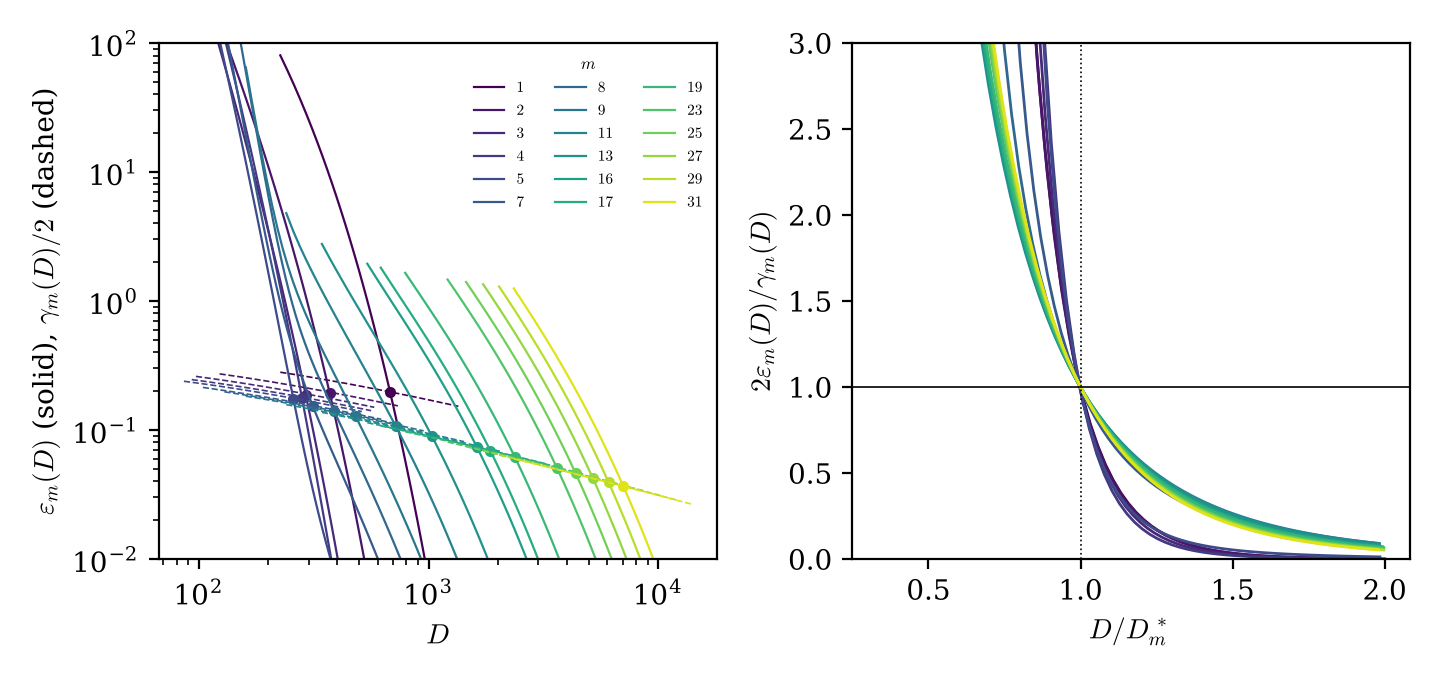
\includegraphics[width=\textwidth]{fig_tail.png}
\caption{Left: the relative error bound $\varepsilon_m(D)$ (solid) and half the relative gap $\gamma_m(D)/2$ (dashed) for $m\in\Mset$; the dots mark $\varepsilon_m(D^*_m)$. Right: the ratio $2\varepsilon_m/\gamma_m$ against $D/D^*_m$. The tail lemma needs this ratio below $1$ at $D^*_m$; Lemmas~\ref{lem:gap} and~\ref{lem:mono} then keep it below $1$ for all larger $D$. For $m\le5$ the class number term $E_3$ dominates the error, for $m\ge7$ the second polar term does.}\label{fig:tail}
\end{figure}

\begin{figure}[ht]\centering
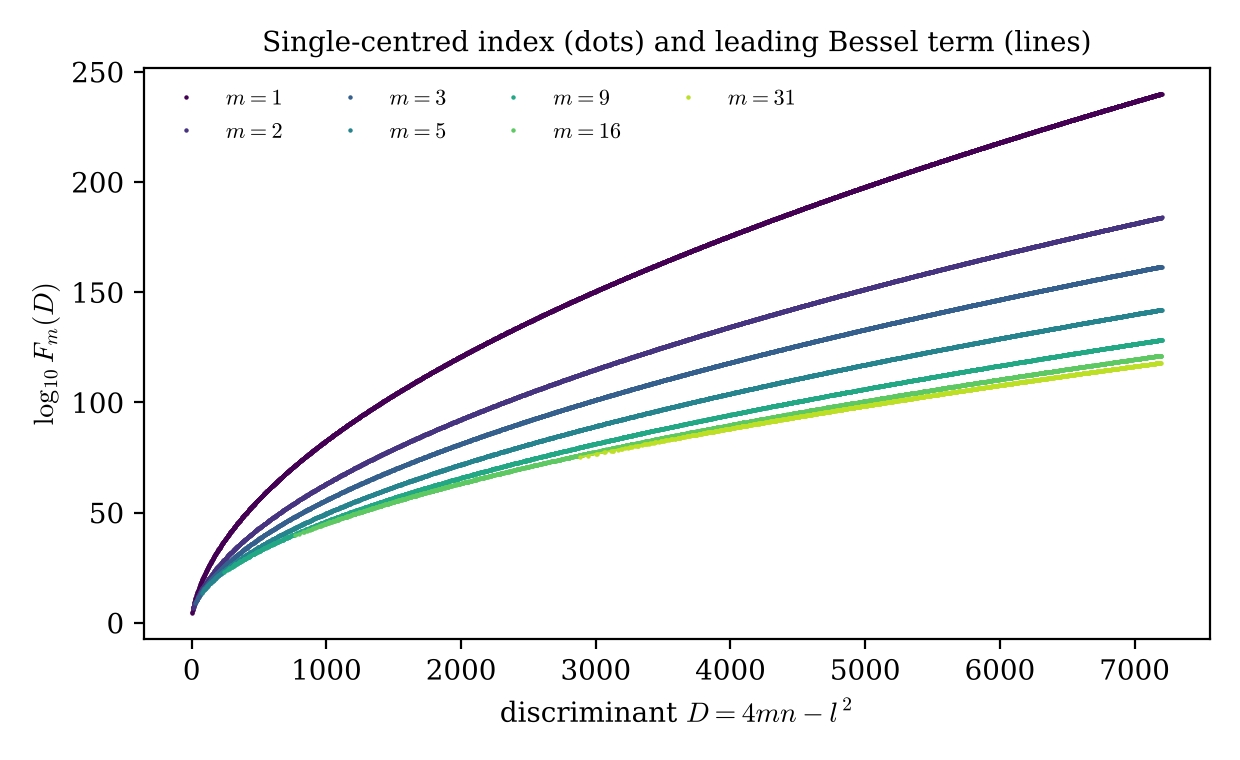
\includegraphics[width=0.86\textwidth]{fig_growth.png}
\caption{The single-centred index $F_m(D)$ at the discriminants of reduced charges with $D\le7200$ (dots), and the main term $T_m(D)$ of \eqref{eq:mainterm} (lines), on a logarithmic scale, for $m=1,2,3,5,9,16,31$. Near $D=7200$ the index has $241$ digits for $m=1$ and $118$ digits for $m=31$; the relative difference between dots and lines is below $\varepsilon_m(D)$ once $D\ge D^*_m$.}\label{fig:growth}
\end{figure}

\section{Proof of Theorem~\ref{thm:B} and Corollary~\ref{cor:C}}\label{sec:proofB}

Let $m\in\Mset$. Define
\[
M_m=\max\Bigl(\max_{\substack{c\le a\le m,\ 0\le b\le c\\4ac-b^2>0}}(-1)^{b+1}\cF_c(a,b),\ \ \max_{\substack{0<D'<D^*_m\\0\le l'\le m}}F_m(D',l')\Bigr),
\]
the second maximum over the pairs with $D'\equiv-l'^2\pmod{4m}$, and let $D_1\ge D^*_m$ be the smallest discriminant of index $m$ such that $F_m(D_1,l_1)>M_m$ for some class $l_1$. These numbers are in Table~\ref{tab:finite}; in every case $D_1+4\le7201$ and $4m^2<D^*_m$.

\begin{table}[ht]\centering
\caption{Data for the proof of Theorem~\ref{thm:B}. The column $F_m(D_1)/M_m$ gives the largest value of $F_m(D_1,l_1)/M_m$ over the classes $l_1$.}\label{tab:finite}
\small
\begin{tabular}{rrrrr@{\qquad}rrrrr}
\toprule
$m$ & $D^*_m$ & $M_m$ & $D_1$ & $F_m(D_1)/M_m$ & $m$ & $D^*_m$ & $M_m$ & $D_1$ & $F_m(D_1)/M_m$\\
\midrule
1 & 680 & $4.69\cdot10^{66}$ & 680 & $1.13$ & 13 & 1030 & $5.87\cdot10^{45}$ & 1031 & $1.19$\\
2 & 371 & $1.59\cdot10^{36}$ & 372 & $1.65$ & 16 & 1624 & $1.03\cdot10^{57}$ & 1628 & $1.25$\\
3 & 292 & $2.45\cdot10^{28}$ & 296 & $1.83$ & 17 & 1857 & $6.78\cdot10^{60}$ & 1868 & $1.63$\\
4 & 281 & $1.67\cdot10^{26}$ & 284 & $1.75$ & 19 & 2375 & $3.25\cdot10^{68}$ & 2375 & $1.13$\\
5 & 258 & $2.24\cdot10^{24}$ & 259 & $1.39$ & 23 & 3630 & $2.00\cdot10^{84}$ & 3631 & $1.09$\\
7 & 313 & $1.30\cdot10^{26}$ & 315 & $1.44$ & 25 & 4370 & $1.88\cdot10^{92}$ & 4371 & $1.15$\\
8 & 388 & $5.95\cdot10^{28}$ & 391 & $1.71$ & 27 & 5185 & $2.50\cdot10^{100}$ & 5192 & $1.18$\\
9 & 481 & $7.44\cdot10^{31}$ & 488 & $1.97$ & 29 & 6079 & $2.84\cdot10^{108}$ & 6083 & $1.34$\\
11 & 720 & $3.02\cdot10^{38}$ & 723 & $1.68$ & 31 & 7052 & $5.40\cdot10^{116}$ & 7052 & $1.08$\\
\bottomrule
\end{tabular}
\end{table}

\begin{proof}[Proof of Theorem~\ref{thm:B}]
Let $n$ and $J\ge0$ be integers with $D=4mn-J^2>0$. If $D\le7200$, then $d(n,J,m)>0$ by Theorem~\ref{thm:A}. Let $D>7200$. Since $4m^2\le3844<D$, Lemma~\ref{lem:secondcharge} shows that the reduced form of $(n,J,m)$ is $[a,b,m]$, so $\dstar(n,J,m)=F_m(D,b)$ by Lemma~\ref{lem:Fwell}. Put $D'=4mn-(J+2)^2=D-4(J+1)$, the discriminant of the second charge.

\emph{Case $D'\le0$.} Then $\dstar(n,J+2,m)=0$ and $d(n,J,m)=\dstar(n,J,m)=F_m(D,b)$, which is positive by \eqref{eq:FT} because $D>D^*_m$ and $\varepsilon_m(D)<\frac12$ (Proposition~\ref{prop:certificate} and Lemma~\ref{lem:mono}).

\emph{Case $D'\ge D^*_m$.} Then $D'>4m^2$, so the reduced form of $(n,J+2,m)$ is $[a',b',m]$ by Lemma~\ref{lem:secondcharge}, and $\dstar(n,J+2,m)=F_m(D',b')$. Since $D'\le D-4$, Theorem~\ref{thm:tail} gives $F_m(D,b)>F_m(D',b')$.

\emph{Case $0<D'<D^*_m$.} By Lemma~\ref{lem:secondcharge}, the reduced form $[a',b',c']$ of $(n,J+2,m)$ has $c'=m$, and then $\dstar(n,J+2,m)=F_m(D',b')\le M_m$, or it has $c'\le a'\le m$, and then $\dstar(n,J+2,m)=(-1)^{b'+1}\cF_{c'}(a',b')\le M_m$. Since $D\ge7201\ge D_1+4$, Theorem~\ref{thm:tail} gives $F_m(D,b)>F_m(D_1,l_1)>M_m\ge\dstar(n,J+2,m)$.

In every case $d(n,J,m)>0$.
\end{proof}

\begin{proof}[Proof of Corollary~\ref{cor:C}]
Let $[a,b,c]$ be the reduced form of $(n,l,m')$, with $c\in\Mset$ and $D>0$. By Lemma~\ref{lem:Fwell}, $\dstar(n,l,m')=F_c(D,b)$. If $D\ge D^*_c$, this is positive by \eqref{eq:FT}, because $\varepsilon_c(D)<\frac12$ by Proposition~\ref{prop:certificate} and Lemma~\ref{lem:mono}. If $D<D^*_c$, then $D<7200$ and $\dstar(n,l,m')>0$ by Theorem~\ref{thm:A}.
\end{proof}

Figure~\ref{fig:index3d} shows the index $d(n,J,7)$ over the region $D\le1000$.

\begin{figure}[ht]\centering
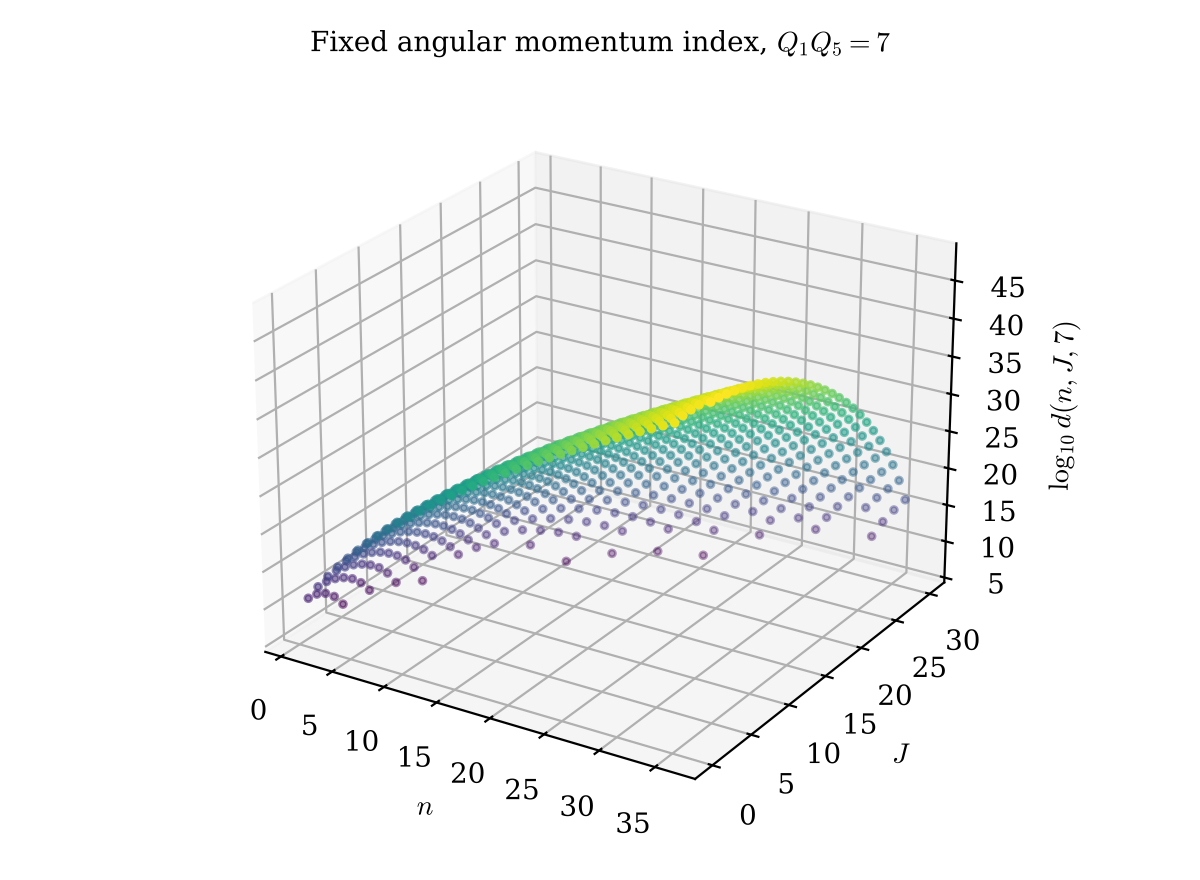
\includegraphics[width=0.78\textwidth]{fig_index3d.png}
\caption{The index at fixed angular momentum $d(n,J,7)$ for all charges with $Q_1Q_5=7$ and $0<4\cdot7\,n-J^2\le1000$, on a logarithmic scale. For fixed $n$ the index falls by many orders of magnitude from small $J$ to the edge $J\approx2\sqrt{7n}$ of the black hole region, following the discriminant $D=28n-J^2$.}\label{fig:index3d}
\end{figure}

\section{Proof of Theorem~\ref{thm:A}}\label{sec:proofA}

\emph{Four dimensions.} Every charge with $0<D\le7200$ has a reduced form $[a,b,c]$ with $0<4ac-b^2\le7200$, and then $3c^2\le D\le7200$ by Lemma~\ref{lem:minima}(iv), so $c\le48$. We computed $\cF_c(a,b)$ exactly for all $c\le49$ and all $(a,b)$ with $4ac-b^2\le7200$ (Appendix~\ref{app:computation}). There are $60\,016$ reduced forms with $0<D\le7200$, and $(-1)^{b+1}\cF_c(a,b)>0$ for each of them.

\emph{Five dimensions.} Let $0<D=4mn-J^2\le7200$. If $4(J+1)\ge D$, the second term of \eqref{eq:drot} vanishes and $d(n,J,m)=\dstar(n,J,m)>0$ by the four-dimensional part. Otherwise $J<D/4\le1800$, and $m$ divides $(D+J^2)/4$; so there are finitely many such charges. For all charges with $0<D\le7200$ and $0\le J\le1801$, $41\,652\,989$ in all, we computed both terms of \eqref{eq:drot} exactly through their reduced forms, and $d(n,J,m)>0$ in every case. \qed

The smallest relative margin $d(n,J,m)/\dstar(n,J,m)$ among these charges is $0.0723$, attained at $m=40$, $n=45$, $J=0$, where $D=7200$. Figure~\ref{fig:margins} shows the margins.

\begin{figure}[ht]\centering
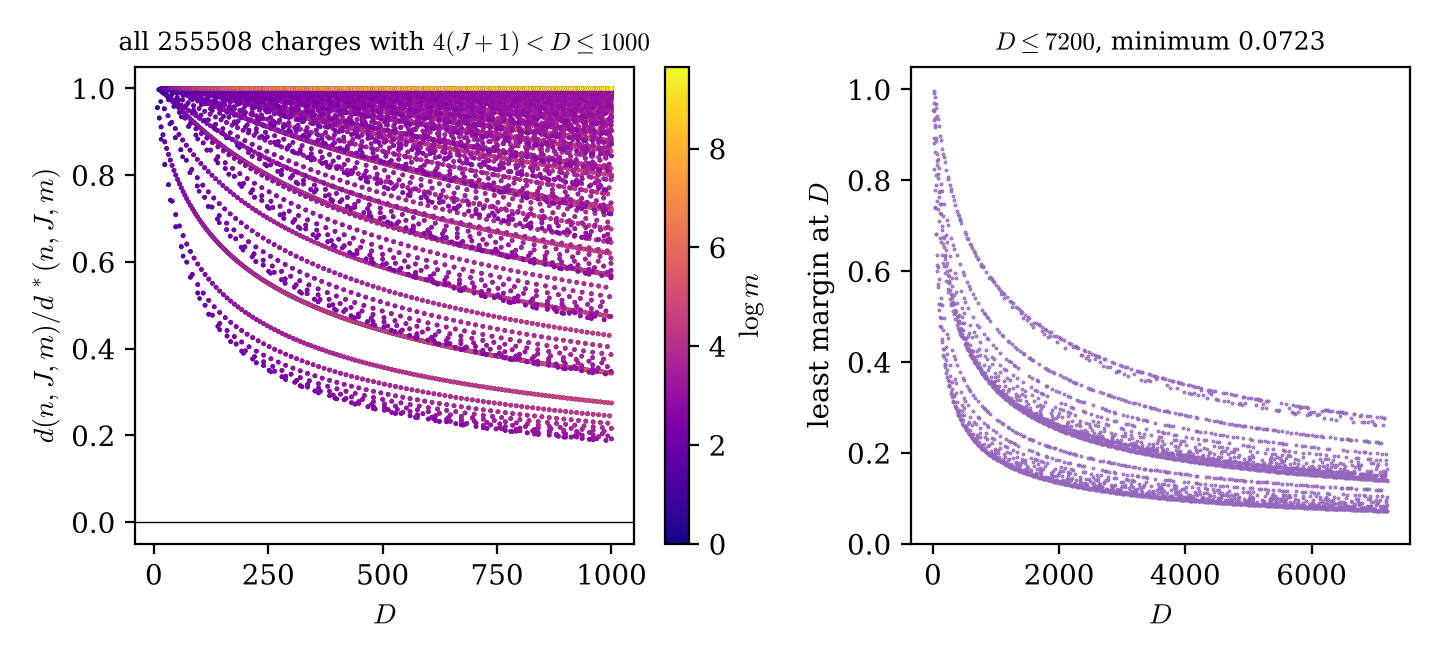
\includegraphics[width=0.86\textwidth]{fig_margins.png}
\caption{Left: the relative margin $d(n,J,m)/\dstar(n,J,m)$ for all five-dimensional charges with $4(J+1)<D\le1000$, coloured by $\log m$; for $4(J+1)\ge D$ the margin is $1$. Right: the least relative margin among all charges of discriminant $D$, for $D\le7200$. The smallest margins occur at $J=0$, where the two discriminants $D$ and $D-4$ are closest.}\label{fig:margins}
\end{figure}

\section{Remarks}\label{sec:remarks}

\subsection*{The reduction cannot be dropped}
If the index at fixed angular momentum is computed from the coefficients of a single function $\psi^F_m$, without passing to reduced forms, one obtains the raw difference $(-1)^{J+1}\bigl(\cF_m(n,J)-\cF_m(n,J+2)\bigr)=F_m(D)-F_m(D-4(J+1))$, where $F_m$ is extended to all $D\equiv-l^2\pmod{4m}$ by Lemma~\ref{lem:Fwell} and by $0$ when the coefficient lies below $n=-1$. Among the charges with $n\ge m$ and $D\le1000$ this raw difference is negative $16$ times for $m=5$ and $26$ times for $m=7$, and it is positive for $m=1,2,3$. The failures occur because $F_m(D)$ is negative at small $D$, for instance $F_5(4)=-2\,023\,536$, or because the second charge is far from reduced. Figure~\ref{fig:raw} compares both prescriptions for $m=5$. This is consistent with the attractor argument of Section~\ref{sec:physics}: only the reduced form of a charge has its attractor point in the chamber where $\psi^F_c$ counts single-centred states.

\begin{figure}[ht]\centering
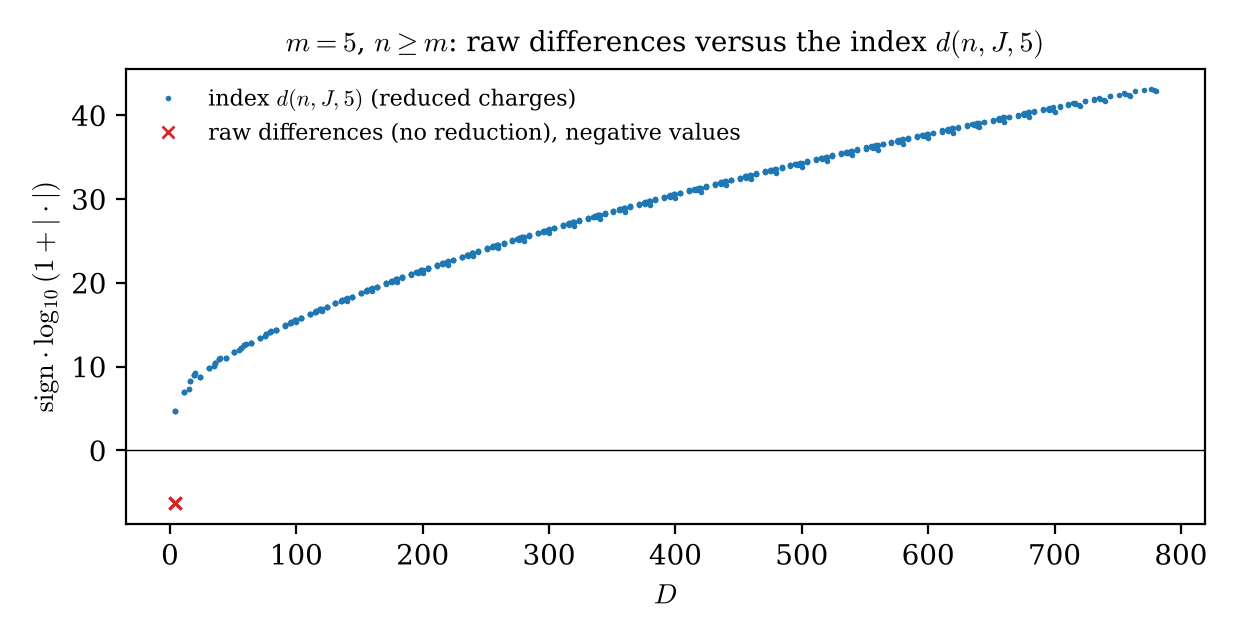
\includegraphics[width=0.86\textwidth]{fig_raw.png}
\caption{For $m=5$ and $n\ge5$: the index $d(n,J,5)$, computed through reduced forms (dots, all positive), and the raw differences of coefficients of $\psi^F_5$ where they are negative (crosses). The vertical axis is $\operatorname{sign}(x)\log_{10}(1+|x|)$.}\label{fig:raw}
\end{figure}

\subsection*{Composite and larger indices}
Two obstacles separate Theorem~\ref{thm:B} from all charges. When $m$ has two distinct prime factors, $\Delta\psi^F_m$ is not a weak Jacobi form plus a combination of the functions $\Hc|V_{m/e^2}|U_e$ (Remark~\ref{rem:composite}); the mock modular correction is then a different object, and we have not determined it. Such $m$ are reached by Theorem~\ref{thm:A} only for $D\le7200$. For prime powers $m\ge32$, Theorem~\ref{thm:D} holds and the tail certificate applies with the same choices, but its threshold grows: it holds at $D^*_{32}=7569$ and $D^*_{37}=10\,456$ and fails one unit below. The next polar term after the most polar one is $(D',l')=(-(m+1)^2,m-1)$, with exponential rate $a_{D'}=\pi(m+1)/m$, and $\alpha_m-a_{D'}=\pi/m+O(m^{-2})$. Its contribution relative to the main term therefore decays only like $e^{-\pi\sqrt D/m}$, the certificate needs $\sqrt{D^*_m}$ to grow at least linearly in $m$, and with it grows the range of discriminants on which the finite part of Section~\ref{sec:proofB} must be computed.

\subsection*{Size of the margins}
The proof of Theorem~\ref{thm:B} is tightest for $m=1$, where $2\varepsilon_1(D^*_1)/\gamma_1(D^*_1)=0.994$; there the error comes from the class number term, whose coefficient $\lambda_1=648$ is large compared with the main term at moderate $D$. For $m\ge7$ the class number term is negligible and the next polar term, at $(D',l')=(-(m+1)^2,m-1)$, limits the estimate. In the finite range the smallest relative margin is $0.0723$ (Section~\ref{sec:proofA}); the index at fixed angular momentum is never close to zero relative to $\dstar$.

\subsection*{Other charges}
Theorems~\ref{thm:A} and~\ref{thm:B} concern charges of torsion one, for which the generating function $1/\Phi_{10}$ is known. For charges of higher torsion, and for the CHL orbifolds of type~II string theory on K3, the method needs two inputs: an analogue of Theorem~\ref{thm:D} that identifies the mock modular part of the finite part, and a tail estimate of the kind proved in Section~\ref{sec:tail}.

\section*{Declarations}

\noindent\textbf{Data availability.} The programs that compute the coefficients $\cF_m(n,l)$, verify the identities of Theorem~\ref{thm:D}, evaluate the tail certificate in ball arithmetic and carry out the finite checks, together with the tables of coefficients they produce, are archived at \url{https://doi.org/\zenodoCodeDOI}.

\smallskip\noindent\textbf{Funding.} This research received no external funding.

\smallskip\noindent\textbf{Conflict of interest.} The author declares no conflict of interest.

\smallskip\noindent\textbf{Ethics.} Not applicable; the work involves no human or animal subjects.

\appendix

\section{Data}\label{app:data}

\subsection*{The weak Jacobi forms \texorpdfstring{$\phi_m$}{phi\_m}}
Write $B=2\phi_{0,1}$. For $m=1$ and prime $m$ the class number term is $\mathcal G_m=\Hc|V_m$, and the forms $\phi_m=\Delta\psi^F_m+\lambda_m\Hc|V_m$ of Theorem~\ref{thm:D} are
\[
\phi_1=3E_4A,\qquad \phi_2=\tfrac{11}{3}E_4AB-\tfrac{10}{3}E_6A^2,
\]
and, for $m=3,5,7,11,13$, the sums of the monomials below with the coefficients beside them.

\medskip
\noindent$m=3$:\nopagebreak\\[2pt]
{\small\begin{tabular}{@{}l@{\ \ }l@{\qquad}l@{\ \ }l@{}}
$E_4 A B^{2}$ & $\tfrac{467}{192}$ & $E_4^{2} A^{3}$ & $\tfrac{203}{48}$ \\
$E_6 A^{2} B$ & $-\tfrac{215}{48}$ & & \\
\end{tabular}}\par\medskip
\noindent$m=5$:\nopagebreak\\[2pt]
{\small\begin{tabular}{@{}l@{\ \ }l@{\qquad}l@{\ \ }l@{}}
$E_4 A B^{4}$ & $\tfrac{72607}{165888}$ & $E_4 E_6 A^{4} B$ & $-\tfrac{1195}{324}$ \\
$E_6 A^{2} B^{3}$ & $-\tfrac{16991}{10368}$ & $E_6^{2} A^{5}$ & $\tfrac{15041}{1296}$ \\
$E_4^{2} A^{3} B^{2}$ & $\tfrac{31561}{6912}$ & $E_4^{3} A^{5}$ & $-\tfrac{10813}{1152}$ \\
\end{tabular}}\par\medskip
\noindent$m=7$:\nopagebreak\\[2pt]
{\small\begin{tabular}{@{}l@{\ \ }l@{\qquad}l@{\ \ }l@{}}
$E_4 A B^{6}$ & $\tfrac{2522801}{63700992}$ & $E_4^{3} A^{5} B^{2}$ & $-\tfrac{1215121}{442368}$ \\
$E_6 A^{2} B^{5}$ & $-\tfrac{397855}{1769472}$ & $E_4^{2} E_6 A^{6} B$ & $-\tfrac{351565}{331776}$ \\
$E_4^{2} A^{3} B^{4}$ & $\tfrac{5487725}{5308416}$ & $E_4 E_6^{2} A^{7}$ & $-\tfrac{1098143}{124416}$ \\
$E_4 E_6 A^{4} B^{3}$ & $-\tfrac{3377833}{1990656}$ & $E_4^{4} A^{7}$ & $\tfrac{356323}{36864}$ \\
$E_6^{2} A^{5} B^{2}$ & $\tfrac{317425}{55296}$ & & \\
\end{tabular}}\par\medskip
\noindent$m=11$:\nopagebreak\\[2pt]
{\small\begin{tabular}{@{}l@{\ \ }l@{\qquad}l@{\ \ }l@{}}
$E_4 A B^{10}$ & $\tfrac{2131467191}{21134460321792}$ & $E_6^{3} A^{8} B^{3}$ & $\tfrac{540339337}{1289945088}$ \\
$E_6 A^{2} B^{9}$ & $-\tfrac{5113428019}{5283615080448}$ & $E_4^{3} E_6 A^{8} B^{3}$ & $-\tfrac{6681275737}{20639121408}$ \\
$E_4^{2} A^{3} B^{8}$ & $\tfrac{13935457241}{1761205026816}$ & $E_4^{2} E_6^{2} A^{9} B^{2}$ & $\tfrac{6195889207}{859963392}$ \\
$E_4 E_6 A^{4} B^{7}$ & $-\tfrac{970619809}{36691771392}$ & $E_4^{5} A^{9} B^{2}$ & $-\tfrac{59476197389}{9172942848}$ \\
$E_6^{2} A^{5} B^{6}$ & $\tfrac{5782066279}{41278242816}$ & $E_4 E_6^{3} A^{10} B$ & $-\tfrac{1053477487}{80621568}$ \\
$E_4^{3} A^{5} B^{6}$ & $-\tfrac{22336678753}{660451885056}$ & $E_4^{4} E_6 A^{10} B$ & $\tfrac{92843167663}{6879707136}$ \\
$E_4^{2} E_6 A^{6} B^{5}$ & $-\tfrac{6566555011}{55037657088}$ & $E_6^{4} A^{11}$ & $\tfrac{404439233}{40310784}$ \\
$E_4 E_6^{2} A^{7} B^{4}$ & $-\tfrac{459938771}{573308928}$ & $E_4^{3} E_6^{2} A^{11}$ & $-\tfrac{4042889417}{322486272}$ \\
$E_4^{4} A^{7} B^{4}$ & $\tfrac{68351027909}{55037657088}$ & $E_4^{6} A^{11}$ & $\tfrac{2092865525}{764411904}$ \\
\end{tabular}}\par\medskip
\noindent$m=13$:\nopagebreak\\[2pt]
{\small\begin{tabular}{@{}l@{\ \ }l@{\qquad}l@{\ \ }l@{}}
$E_4 A B^{12}$ & $\tfrac{21052966501}{6086724572676096}$ & $E_4^{5} A^{9} B^{4}$ & $-\tfrac{168553028141}{293534171136}$ \\
$E_6 A^{2} B^{11}$ & $-\tfrac{1691946635}{42268920643584}$ & $E_4 E_6^{3} A^{10} B^{3}$ & $-\tfrac{37682583031}{46438023168}$ \\
$E_4^{2} A^{3} B^{10}$ & $\tfrac{101024148481}{253613523861504}$ & $E_4^{4} E_6 A^{10} B^{3}$ & $\tfrac{62552439743}{55037657088}$ \\
$E_4 E_6 A^{4} B^{9}$ & $-\tfrac{39816293555}{23776267862016}$ & $E_6^{4} A^{11} B^{2}$ & $\tfrac{1064334965}{1289945088}$ \\
$E_6^{2} A^{5} B^{8}$ & $\tfrac{16000805975}{1761205026816}$ & $E_4^{3} E_6^{2} A^{11} B^{2}$ & $-\tfrac{15342776135}{6879707136}$ \\
$E_4^{3} A^{5} B^{8}$ & $-\tfrac{7084900171}{14089640214528}$ & $E_4^{6} A^{11} B^{2}$ & $\tfrac{7920621283}{4076863488}$ \\
$E_4^{2} E_6 A^{6} B^{7}$ & $-\tfrac{17239195301}{1320903770112}$ & $E_4^{2} E_6^{3} A^{12} B$ & $\tfrac{22105328483}{7739670528}$ \\
$E_4 E_6^{2} A^{7} B^{6}$ & $-\tfrac{25730368859}{990677827584}$ & $E_4^{5} E_6 A^{12} B$ & $-\tfrac{38847685}{15925248}$ \\
$E_4^{4} A^{7} B^{6}$ & $\tfrac{81058056707}{880602513408}$ & $E_4 E_6^{4} A^{13}$ & $-\tfrac{903349379}{362797056}$ \\
$E_6^{3} A^{8} B^{5}$ & $-\tfrac{507482165}{13759414272}$ & $E_4^{4} E_6^{2} A^{13}$ & $\tfrac{8275754885}{2293235712}$ \\
$E_4^{3} E_6 A^{8} B^{5}$ & $\tfrac{3161174131}{55037657088}$ & $E_4^{7} A^{13}$ & $-\tfrac{1929616631}{2038431744}$ \\
$E_4^{2} E_6^{2} A^{9} B^{4}$ & $\tfrac{139668317891}{165112971264}$ & & \\
\end{tabular}}\par\medskip

The constants are $\lambda_1=648$, $\lambda_2=3200$, $\lambda_3=25650$, $\lambda_5=1073720$, $\lambda_7=30178575$, $\lambda_{11}=10914317934$ and $\lambda_{13}=156883829400$; for $m\ge2$ they are $\pf(m+1)$, and the linear algebra of Section~\ref{sec:completion} recovers each of them as the coefficient of $\mathcal G_m$.

\subsection*{Polar terms}
The polar terms $(D',l')$, $0\le l'\le m$, of $\phi_m/\Delta$ and the coefficients $a_m(D',l')$ entering \eqref{eq:rademacher} are listed below. The first entry is the most polar term $(-m(m+4),m)$ with coefficient $m+2$. An entry with $-4m\le D'<0$ differs from the corresponding coefficient of $\psi^F_m$ by $\lambda_m\delta_m(D',l')$, the contribution of the class number form $\lambda_mG_m$; in particular the entry $(-4m,0)$ receives $\lambda_m g_m(0,0)$, which by $H(0)=-1/12$ equals $-\lambda_m\sigma(m)/12$ for $m=1$ and $m$ prime, and $-\lambda_m\bigl(\sigma(p^k)-p\,\sigma(p^{k-2})\bigr)/12$ for $m=p^k$ with $k\ge2$. All other entries are coefficients of $\psi^F_m$.

\medskip

\noindent$m=1$:\nopagebreak\\[2pt]
{\small\begin{tabular}{@{}r@{\ \ }r@{\qquad}r@{\ \ }r@{\qquad}r@{\ \ }r@{}}
$(-5,1)$ & $3$ & $(-4,0)$ & $-6$ & $(-1,1)$ & $816$ \\
\end{tabular}}\par\medskip
\noindent$m=2$:\nopagebreak\\[2pt]
{\small\begin{tabular}{@{}r@{\ \ }r@{\qquad}r@{\ \ }r@{\qquad}r@{\ \ }r@{}}
$(-12,2)$ & $4$ & $(-8,0)$ & $-152$ & $(-1,1)$ & $11576$ \\
$(-9,1)$ & $72$ & $(-4,2)$ & $2752$ & & \\
\end{tabular}}\par\medskip
\noindent$m=3$:\nopagebreak\\[2pt]
{\small\begin{tabular}{@{}r@{\ \ }r@{\qquad}r@{\ \ }r@{\qquad}r@{\ \ }r@{}}
$(-21,3)$ & $5$ & $(-12,0)$ & $-2146$ & $(-1,1)$ & $110826$ \\
$(-16,2)$ & $96$ & $(-9,3)$ & $10278$ & & \\
$(-13,1)$ & $972$ & $(-4,2)$ & $41250$ & & \\
\end{tabular}}\par\medskip
\noindent$m=4$:\nopagebreak\\[2pt]
{\small\begin{tabular}{@{}r@{\ \ }r@{\qquad}r@{\ \ }r@{\qquad}r@{\ \ }r@{}}
$(-32,4)$ & $6$ & $(-17,1)$ & $9600$ & $(-9,3)$ & $199584$ \\
$(-25,3)$ & $120$ & $(-16,0)$ & $-22044$ & $(-4,2)$ & $272256$ \\
$(-20,2)$ & $1296$ & $(-16,4)$ & $16992$ & $(-1,1)$ & $1053288$ \\
\end{tabular}}\par\medskip
\noindent$m=5$:\nopagebreak\\[2pt]
{\small\begin{tabular}{@{}r@{\ \ }r@{\qquad}r@{\ \ }r@{\qquad}r@{\ \ }r@{}}
$(-45,5)$ & $7$ & $(-24,2)$ & $12800$ & $(-9,3)$ & $1304192$ \\
$(-36,4)$ & $144$ & $(-21,1)$ & $76955$ & $(-5,5)$ & $2462695$ \\
$(-29,3)$ & $1620$ & $(-20,0)$ & $-183052$ & $(-4,2)$ & $2857380$ \\
$(-25,5)$ & $2880$ & $(-16,4)$ & $567964$ & $(-1,1)$ & $6004640$ \\
\end{tabular}}\par\medskip
\noindent$m=7$:\nopagebreak\\[2pt]
{\small\begin{tabular}{@{}r@{\ \ }r@{\qquad}r@{\ \ }r@{\qquad}r@{\ \ }r@{}}
$(-77,7)$ & $9$ & $(-36,6)$ & $46656$ & $(-16,4)$ & $42700596$ \\
$(-64,6)$ & $192$ & $(-32,2)$ & $705030$ & $(-9,3)$ & $42892335$ \\
$(-53,5)$ & $2268$ & $(-29,1)$ & $3222780$ & $(-8,6)$ & $64504998$ \\
$(-49,7)$ & $4032$ & $(-28,0)$ & $-8155458$ & $(-4,2)$ & $113142510$ \\
$(-44,4)$ & $19200$ & $(-25,5)$ & $10443525$ & $(-1,1)$ & $213270204$ \\
$(-37,3)$ & $128250$ & $(-21,7)$ & $30703455$ & & \\
\end{tabular}}\par\medskip
\noindent$m=8$:\nopagebreak\\[2pt]
{\small\begin{tabular}{@{}r@{\ \ }r@{\qquad}r@{\ \ }r@{\qquad}r@{\ \ }r@{}}
$(-96,8)$ & $10$ & $(-41,3)$ & $881280$ & $(-17,7)$ & $291552000$ \\
$(-81,7)$ & $216$ & $(-36,2)$ & $4295024$ & $(-16,4)$ & $88514880$ \\
$(-68,6)$ & $2592$ & $(-36,6)$ & $460800$ & $(-9,3)$ & $507090312$ \\
$(-64,8)$ & $4608$ & $(-33,1)$ & $17807488$ & $(-4,2)$ & $293278848$ \\
$(-57,5)$ & $22400$ & $(-32,0)$ & $-46325820$ & $(-4,6)$ & $319626000$ \\
$(-49,7)$ & $54432$ & $(-32,8)$ & $36425856$ & $(-1,1)$ & $1326869904$ \\
$(-48,4)$ & $153900$ & $(-25,5)$ & $146262000$ & & \\
\end{tabular}}\par\medskip
\noindent$m=9$:\nopagebreak\\[2pt]
{\small\begin{tabular}{@{}r@{\ \ }r@{\qquad}r@{\ \ }r@{\qquad}r@{\ \ }r@{}}
$(-117,9)$ & $11$ & $(-49,7)$ & $537600$ & $(-25,5)$ & $660400140$ \\
$(-100,8)$ & $240$ & $(-45,3)$ & $5368607$ & $(-16,4)$ & $1381606824$ \\
$(-85,7)$ & $2916$ & $(-45,9)$ & $734832$ & $(-13,7)$ & $1959301872$ \\
$(-81,9)$ & $5184$ & $(-40,2)$ & $23723928$ & $(-9,3)$ & $641927340$ \\
$(-72,6)$ & $25600$ & $(-37,1)$ & $90663975$ & $(-9,9)$ & $903535672$ \\
$(-64,8)$ & $62208$ & $(-36,0)$ & $-242044726$ & $(-4,2)$ & $3419104860$ \\
$(-61,5)$ & $179550$ & $(-36,6)$ & $110235150$ & $(-1,1)$ & $5612232504$ \\
$(-52,4)$ & $1057536$ & $(-28,8)$ & $645470100$ & & \\
\end{tabular}}\par\medskip
\noindent$m=11$:\nopagebreak\\[2pt]
{\small\begin{tabular}{@{}r@{\ \ }r@{\qquad}r@{\ \ }r@{\qquad}r@{\ \ }r@{}}
$(-165,11)$ & $13$ & $(-69,5)$ & $7516040$ & $(-36,6)$ & $11068933758$ \\
$(-144,10)$ & $288$ & $(-64,8)$ & $4924800$ & $(-33,11)$ & $10985997934$ \\
$(-125,9)$ & $3564$ & $(-60,4)$ & $35582984$ & $(-25,5)$ & $11626016334$ \\
$(-121,11)$ & $6336$ & $(-56,10)$ & $8294400$ & $(-20,8)$ & $22171278828$ \\
$(-108,8)$ & $32000$ & $(-53,3)$ & $150895143$ & $(-16,4)$ & $24728241564$ \\
$(-100,10)$ & $77760$ & $(-49,7)$ & $29611008$ & $(-12,10)$ & $33235440206$ \\
$(-93,7)$ & $230850$ & $(-48,2)$ & $572889900$ & $(-9,3)$ & $32215422180$ \\
$(-81,9)$ & $691200$ & $(-45,1)$ & $1923116507$ & $(-5,7)$ & $45397013391$ \\
$(-80,6)$ & $1410048$ & $(-44,0)$ & $-5383354674$ & $(-4,2)$ & $54013959228$ \\
$(-77,11)$ & $944784$ & $(-37,9)$ & $10972492134$ & $(-1,1)$ & $95512792158$ \\
\end{tabular}}\par\medskip
\noindent$m=13$:\nopagebreak\\[2pt]
{\small\begin{tabular}{@{}r@{\ \ }r@{\qquad}r@{\ \ }r@{\qquad}r@{\ \ }r@{}}
$(-221,13)$ & $15$ & $(-88,6)$ & $47443968$ & $(-40,12)$ & $209835079200$ \\
$(-196,12)$ & $336$ & $(-81,9)$ & $38071296$ & $(-36,6)$ & $239671505556$ \\
$(-173,11)$ & $4212$ & $(-77,5)$ & $211250034$ & $(-29,9)$ & $473086686780$ \\
$(-169,13)$ & $7488$ & $(-69,11)$ & $74795400$ & $(-25,5)$ & $226363597200$ \\
$(-152,10)$ & $38400$ & $(-68,4)$ & $859106592$ & $(-17,11)$ & $317715802800$ \\
$(-144,12)$ & $93312$ & $(-65,13)$ & $92160000$ & $(-16,4)$ & $453680614524$ \\
$(-133,9)$ & $282150$ & $(-64,8)$ & $206154240$ & $(-13,13)$ & $632140801722$ \\
$(-121,11)$ & $844800$ & $(-61,3)$ & $3196426050$ & $(-12,8)$ & $325296962928$ \\
$(-117,13)$ & $1154736$ & $(-56,2)$ & $10826901840$ & $(-9,3)$ & $353837671920$ \\
$(-116,8)$ & $1762560$ & $(-53,1)$ & $32893848945$ & $(-4,2)$ & $1079018682192$ \\
$(-101,7)$ & $9663480$ & $(-52,0)$ & $-96093457164$ & $(-1,1)$ & $1672865232240$ \\
$(-100,10)$ & $6156000$ & $(-49,7)$ & $53290933296$ & & \\
$(-92,12)$ & $10368000$ & $(-48,10)$ & $78898770252$ & & \\
\end{tabular}}\par\medskip
\noindent$m=16$:\nopagebreak\\[2pt]
{\scriptsize\begin{tabular}{@{}r@{\ \ }r@{\qquad}r@{\ \ }r@{}}
$(-320,16)$ & $18$ & $(-81,9)$ & $6518572200$ \\
$(-289,15)$ & $408$ & $(-80,4)$ & $65487317652$ \\
$(-260,14)$ & $5184$ & $(-80,12)$ & $3478852800$ \\
$(-256,16)$ & $9216$ & $(-73,3)$ & $210990569472$ \\
$(-233,13)$ & $48000$ & $(-68,2)$ & $628394424192$ \\
$(-225,15)$ & $116640$ & $(-68,14)$ & $5640192000$ \\
$(-208,12)$ & $359100$ & $(-65,1)$ & $1702877026944$ \\
$(-196,14)$ & $1075200$ & $(-64,0)$ & $-5266940863488$ \\
$(-192,16)$ & $1469664$ & $(-64,8)$ & $577459667808$ \\
$(-185,11)$ & $2291328$ & $(-64,16)$ & $3856357571400$ \\
$(-169,13)$ & $8002800$ & $(-57,11)$ & $6616913348736$ \\
$(-164,10)$ & $12884640$ & $(-49,7)$ & $13306634464800$ \\
$(-161,15)$ & $13478400$ & $(-41,13)$ & $19829783203200$ \\
$(-145,9)$ & $65235456$ & $(-36,6)$ & $389561923584$ \\
$(-144,12)$ & $50761728$ & $(-36,10)$ & $13277462957856$ \\
$(-132,14)$ & $99727200$ & $(-33,15)$ & $19839548764800$ \\
$(-128,8)$ & $301785750$ & $(-25,5)$ & $27708909940080$ \\
$(-128,16)$ & $122880000$ & $(-17,9)$ & $33322846608000$ \\
$(-121,11)$ & $283462080$ & $(-16,4)$ & $8463731143680$ \\
$(-113,7)$ & $1288656000$ & $(-16,12)$ & $4551567686400$ \\
$(-105,13)$ & $628176384$ & $(-9,3)$ & $37891069648920$ \\
$(-100,6)$ & $5113994640$ & $(-4,2)$ & $29191726062720$ \\
$(-100,10)$ & $1423319040$ & $(-4,14)$ & $26618808680400$ \\
$(-97,15)$ & $902880000$ & $(-1,1)$ & $98600177562696$ \\
$(-89,5)$ & $18935832960$ & & \\
\end{tabular}}\par\medskip
\noindent$m=17$:\nopagebreak\\[2pt]
{\scriptsize\begin{tabular}{@{}r@{\ \ }r@{\qquad}r@{\ \ }r@{}}
$(-357,17)$ & $19$ & $(-93,5)$ & $76400456388$ \\
$(-324,16)$ & $432$ & $(-89,15)$ & $6204211200$ \\
$(-293,15)$ & $5508$ & $(-85,17)$ & $7237147500$ \\
$(-289,17)$ & $9792$ & $(-84,4)$ & $253147456960$ \\
$(-264,14)$ & $51200$ & $(-81,9)$ & $30927744216$ \\
$(-256,16)$ & $124416$ & $(-77,3)$ & $784630397034$ \\
$(-237,13)$ & $384750$ & $(-76,12)$ & $19214807040$ \\
$(-225,15)$ & $1152000$ & $(-72,2)$ & $2256302479736$ \\
$(-221,17)$ & $1574640$ & $(-69,1)$ & $5924949883415$ \\
$(-212,12)$ & $2467584$ & $(-68,0)$ & $-18649353355308$ \\
$(-196,14)$ & $8618400$ & $(-64,8)$ & $10948398535908$ \\
$(-189,11)$ & $13958360$ & $(-60,14)$ & $21685684256200$ \\
$(-188,16)$ & $14515200$ & $(-53,11)$ & $43390651159368$ \\
$(-169,13)$ & $54991872$ & $(-52,16)$ & $32522197488300$ \\
$(-168,10)$ & $71165952$ & $(-49,7)$ & $22105788825240$ \\
$(-157,15)$ & $108037800$ & $(-36,6)$ & $66525792046920$ \\
$(-153,17)$ & $133120000$ & $(-33,13)$ & $43473448733200$ \\
$(-149,9)$ & $331964325$ & $(-32,10)$ & $54499446598356$ \\
$(-144,12)$ & $309231360$ & $(-25,5)$ & $26717724373200$ \\
$(-132,8)$ & $1431840000$ & $(-21,15)$ & $108504494419955$ \\
$(-128,14)$ & $685283328$ & $(-17,17)$ & $43582246216080$ \\
$(-121,11)$ & $1565650944$ & $(-16,4)$ & $58424969095824$ \\
$(-120,16)$ & $984960000$ & $(-13,9)$ & $88055159831172$ \\
$(-117,7)$ & $5753243711$ & $(-9,3)$ & $106294598576208$ \\
$(-104,6)$ & $21640922280$ & $(-8,12)$ & $87377876532648$ \\
$(-101,13)$ & $3826738080$ & $(-4,2)$ & $177792067095372$ \\
$(-100,10)$ & $7242858000$ & $(-1,1)$ & $245644283204496$ \\
\end{tabular}}\par\medskip
\noindent$m=19$:\nopagebreak\\[2pt]
{\scriptsize\begin{tabular}{@{}r@{\ \ }r@{\qquad}r@{\ \ }r@{}}
$(-437,19)$ & $21$ & $(-121,11)$ & $37800576000$ \\
$(-400,18)$ & $480$ & $(-120,14)$ & $23057768448$ \\
$(-365,17)$ & $6156$ & $(-112,6)$ & $337518746100$ \\
$(-361,19)$ & $10944$ & $(-104,16)$ & $41230848000$ \\
$(-332,16)$ & $57600$ & $(-101,5)$ & $1098196469280$ \\
$(-324,18)$ & $139968$ & $(-100,10)$ & $153419832240$ \\
$(-301,15)$ & $436050$ & $(-96,18)$ & $54251596800$ \\
$(-289,17)$ & $1305600$ & $(-93,13)$ & $107556441300$ \\
$(-285,19)$ & $1784592$ & $(-92,4)$ & $3378941866104$ \\
$(-272,14)$ & $2820096$ & $(-85,3)$ & $9788426044191$ \\
$(-256,16)$ & $9849600$ & $(-81,9)$ & $584304884064$ \\
$(-248,18)$ & $16588800$ & $(-80,2)$ & $26463967407252$ \\
$(-245,13)$ & $16105800$ & $(-77,1)$ & $65738606045634$ \\
$(-225,15)$ & $63452160$ & $(-76,0)$ & $-213880362634530$ \\
$(-220,12)$ & $83026944$ & $(-73,15)$ & $72244992982950$ \\
$(-213,17)$ & $124659000$ & $(-68,12)$ & $216572634733842$ \\
$(-209,19)$ & $153600000$ & $(-64,8)$ & $290240512063128$ \\
$(-197,11)$ & $392321475$ & $(-61,17)$ & $432520387240500$ \\
$(-196,14)$ & $360769920$ & $(-57,19)$ & $216450446524146$ \\
$(-180,16)$ & $799497216$ & $(-49,7)$ & $295233026761560$ \\
$(-176,10)$ & $1718208000$ & $(-45,11)$ & $650190207407382$ \\
$(-172,18)$ & $1149120000$ & $(-44,14)$ & $649291870132950$ \\
$(-169,13)$ & $1850314752$ & $(-36,6)$ & $454813054337556$ \\
$(-157,9)$ & $7031742300$ & $(-28,16)$ & $721883567564100$ \\
$(-149,15)$ & $4522508640$ & $(-25,5)$ & $499868176959420$ \\
$(-144,12)$ & $8691429600$ & $(-24,10)$ & $439229144775060$ \\
$(-140,8)$ & $27051148812$ & $(-20,18)$ & $866327370562008$ \\
$(-137,17)$ & $7332249600$ & $(-17,13)$ & $652449860097750$ \\
$(-133,19)$ & $8552992500$ & $(-16,4)$ & $1053337413298920$ \\
$(-125,7)$ & $98228864970$ & $(-9,3)$ & $702773949743370$ \\
\end{tabular}}\par
{\scriptsize\begin{tabular}{@{}r@{\ \ }r@{\qquad}r@{\ \ }r@{}}
$(-5,9)$ & $1537516442814717$ & $(-1,1)$ & $2909367756476946$ \\
$(-4,2)$ & $1789602194930022$ & & \\
\end{tabular}}\par\medskip
\noindent$m=23$:\nopagebreak\\[2pt]
{\scriptsize\begin{tabular}{@{}r@{\ \ }r@{\qquad}r@{\ \ }r@{}}
$(-621,23)$ & $25$ & $(-225,15)$ & $51546240000$ \\
$(-576,22)$ & $576$ & $(-216,20)$ & $54974464000$ \\
$(-533,21)$ & $7452$ & $(-213,11)$ & $141886133142$ \\
$(-529,23)$ & $13248$ & $(-208,22)$ & $72335462400$ \\
$(-492,20)$ & $70400$ & $(-197,17)$ & $146667874500$ \\
$(-484,22)$ & $171072$ & $(-196,14)$ & $214787764800$ \\
$(-453,19)$ & $538650$ & $(-192,10)$ & $506277734414$ \\
$(-441,21)$ & $1612800$ & $(-177,19)$ & $284663808000$ \\
$(-437,23)$ & $2204496$ & $(-173,9)$ & $1725722127612$ \\
$(-416,18)$ & $3525120$ & $(-169,13)$ & $843995842560$ \\
$(-400,20)$ & $12312000$ & $(-165,21)$ & $413113770000$ \\
$(-392,22)$ & $20736000$ & $(-164,16)$ & $649482624000$ \\
$(-381,17)$ & $20400680$ & $(-161,23)$ & $465992663040$ \\
$(-361,19)$ & $80372736$ & $(-156,8)$ & $5631167703640$ \\
$(-349,21)$ & $157901400$ & $(-144,12)$ & $3143323565280$ \\
$(-348,16)$ & $106748928$ & $(-141,7)$ & $17611124144035$ \\
$(-345,23)$ & $194560000$ & $(-140,18)$ & $1352000160000$ \\
$(-324,18)$ & $463847040$ & $(-133,15)$ & $2692518051600$ \\
$(-317,15)$ & $513035775$ & $(-128,6)$ & $52797261964950$ \\
$(-308,20)$ & $1027924992$ & $(-124,20)$ & $2129641113600$ \\
$(-300,22)$ & $1477440000$ & $(-121,11)$ & $11138110242336$ \\
$(-289,17)$ & $2419642368$ & $(-117,5)$ & $151565029757111$ \\
$(-288,14)$ & $2290944000$ & $(-116,22)$ & $2649494292480$ \\
$(-269,19)$ & $5914049760$ & $(-108,4)$ & $415459643733872$ \\
$(-261,13)$ & $9588739500$ & $(-105,17)$ & $5956454400000$ \\
$(-257,21)$ & $9588326400$ & $(-104,14)$ & $10517486656680$ \\
$(-256,16)$ & $11588572800$ & $(-101,3)$ & $1081641789325530$ \\
$(-253,23)$ & $11184682500$ & $(-100,10)$ & $37652125212000$ \\
$(-236,12)$ & $37871608320$ & $(-96,2)$ & $2650308467184860$ \\
$(-232,18)$ & $30743691264$ & $(-93,1)$ & $6022732288717356$ \\
\end{tabular}}\par
{\scriptsize\begin{tabular}{@{}r@{\ \ }r@{\qquad}r@{\ \ }r@{}}
$(-92,0)$ & $-20800342108291896$ & $(-36,6)$ & $69560999106618720$ \\
$(-85,19)$ & $16620472160605650$ & $(-32,20)$ & $66505466318775030$ \\
$(-81,9)$ & $16732042562445564$ & $(-29,11)$ & $83509521255588480$ \\
$(-77,13)$ & $33259716859605360$ & $(-25,5)$ & $24936698942625900$ \\
$(-73,21)$ & $16623997826310588$ & $(-24,22)$ & $66518048767229280$ \\
$(-72,16)$ & $33245365402689400$ & $(-16,4)$ & $87376975980941520$ \\
$(-69,23)$ & $49846214714614900$ & $(-13,17)$ & $83232409805408472$ \\
$(-64,8)$ & $33596527753603512$ & $(-12,14)$ & $100011713355005804$ \\
$(-52,12)$ & $33357513284316600$ & $(-9,3)$ & $98925661825643628$ \\
$(-49,7)$ & $17719252672955100$ & $(-8,10)$ & $67901293719386976$ \\
$(-48,18)$ & $66485708494441500$ & $(-4,2)$ & $139365700955059560$ \\
$(-41,15)$ & $33316038280577400$ & $(-1,1)$ & $242591082794658480$ \\
\end{tabular}}\par\medskip
\noindent$m=25$:\nopagebreak\\[2pt]
{\scriptsize\begin{tabular}{@{}r@{\ \ }r@{\qquad}r@{\ \ }r@{}}
$(-725,25)$ & $27$ & $(-289,17)$ & $58419072000$ \\
$(-676,24)$ & $624$ & $(-284,22)$ & $61846272000$ \\
$(-629,23)$ & $8100$ & $(-276,24)$ & $81377395200$ \\
$(-625,25)$ & $14400$ & $(-269,13)$ & $163714769010$ \\
$(-584,22)$ & $76800$ & $(-261,19)$ & $166223591100$ \\
$(-576,24)$ & $186624$ & $(-256,16)$ & $245471731200$ \\
$(-541,21)$ & $589950$ & $(-244,12)$ & $590657356800$ \\
$(-529,23)$ & $1766400$ & $(-241,21)$ & $322618982400$ \\
$(-525,25)$ & $2414448$ & $(-229,23)$ & $468195606000$ \\
$(-500,20)$ & $3877632$ & $(-225,15)$ & $973841356800$ \\
$(-484,22)$ & $13543200$ & $(-225,25)$ & $528125018112$ \\
$(-476,24)$ & $22809600$ & $(-224,18)$ & $742265856000$ \\
$(-461,19)$ & $22548120$ & $(-221,11)$ & $2039489782215$ \\
$(-441,21)$ & $88833024$ & $(-200,10)$ & $6757400879544$ \\
$(-429,23)$ & $174522600$ & $(-200,20)$ & $1545143040000$ \\
$(-425,25)$ & $215040000$ & $(-196,14)$ & $3667210825824$ \\
$(-424,18)$ & $118609920$ & $(-189,17)$ & $3106751598000$ \\
$(-400,20)$ & $515385600$ & $(-184,22)$ & $2433875558400$ \\
$(-389,17)$ & $573392925$ & $(-181,9)$ & $21524693185035$ \\
$(-384,22)$ & $1142138880$ & $(-176,24)$ & $3027993477120$ \\
$(-376,24)$ & $1641600000$ & $(-169,13)$ & $13163221094712$ \\
$(-361,19)$ & $2704306176$ & $(-164,8)$ & $65996213108640$ \\
$(-356,16)$ & $2577312000$ & $(-161,19)$ & $6872832000000$ \\
$(-341,21)$ & $6609820320$ & $(-156,16)$ & $12270401095680$ \\
$(-329,23)$ & $10716364800$ & $(-149,7)$ & $194862258910125$ \\
$(-325,15)$ & $10867238100$ & $(-144,12)$ & $45182542960512$ \\
$(-325,25)$ & $12500527500$ & $(-141,21)$ & $11611206731250$ \\
$(-324,18)$ & $13037144400$ & $(-136,6)$ & $553836164704200$ \\
$(-300,20)$ & $34586652672$ & $(-129,23)$ & $15679282544640$ \\
$(-296,14)$ & $43281838080$ & $(-125,5)$ & $1512859258863720$ \\
\end{tabular}}\par
{\scriptsize\begin{tabular}{@{}r@{\ \ }r@{\qquad}r@{\ \ }r@{}}
$(-125,15)$ & $45971107141572$ & $(-64,8)$ & $330062565925438758$ \\
$(-125,25)$ & $17293119576000$ & $(-61,19)$ & $521661779676065430$ \\
$(-124,18)$ & $28638368640000$ & $(-56,16)$ & $521867731813760880$ \\
$(-121,11)$ & $148662826021776$ & $(-49,7)$ & $272356569849859560$ \\
$(-116,4)$ & $3959104942633920$ & $(-44,12)$ & $523273123016135280$ \\
$(-109,3)$ & $9871029907055100$ & $(-41,21)$ & $391414548006833940$ \\
$(-104,2)$ & $23235254202421080$ & $(-36,6)$ & $487409795338655826$ \\
$(-101,1)$ & $50912869133641230$ & $(-29,23)$ & $912956331911761320$ \\
$(-100,0)$ & $-180673890965605794$ & $(-25,5)$ & $166300240644599760$ \\
$(-100,10)$ & $43923681752975940$ & $(-25,15)$ & $88393185594933480$ \\
$(-100,20)$ & $43505469207466740$ & $(-25,25)$ & $87365323849071072$ \\
$(-96,14)$ & $65345111736595470$ & $(-24,18)$ & $522281256406728480$ \\
$(-89,17)$ & $130474688278237020$ & $(-21,11)$ & $657516846337463340$ \\
$(-84,22)$ & $195617701417613130$ & $(-16,4)$ & $712803047925978480$ \\
$(-81,9)$ & $131787679942610820$ & $(-9,3)$ & $692666646950331360$ \\
$(-76,24)$ & $260813458688712120$ & $(-4,2)$ & $1685617453229768280$ \\
$(-69,13)$ & $391645600540377660$ & $(-1,1)$ & $2125330279004749164$ \\
\end{tabular}}\par\medskip
\noindent$m=27$:\nopagebreak\\[2pt]
{\scriptsize\begin{tabular}{@{}r@{\ \ }r@{\qquad}r@{\ \ }r@{}}
$(-837,27)$ & $29$ & $(-361,19)$ & $65291904000$ \\
$(-784,26)$ & $672$ & $(-360,24)$ & $68718080000$ \\
$(-733,25)$ & $8748$ & $(-352,26)$ & $90419328000$ \\
$(-729,27)$ & $15552$ & $(-333,15)$ & $185543404878$ \\
$(-684,24)$ & $83200$ & $(-333,21)$ & $185779307700$ \\
$(-676,26)$ & $202176$ & $(-324,18)$ & $276155697600$ \\
$(-637,23)$ & $641250$ & $(-313,23)$ & $360574156800$ \\
$(-625,25)$ & $1920000$ & $(-304,14)$ & $675036979200$ \\
$(-621,27)$ & $2624400$ & $(-301,25)$ & $523277442000$ \\
$(-592,22)$ & $4230144$ & $(-297,27)$ & $590257373184$ \\
$(-576,24)$ & $14774400$ & $(-292,20)$ & $835049088000$ \\
$(-568,26)$ & $24883200$ & $(-289,17)$ & $1103686871040$ \\
$(-549,21)$ & $24695560$ & $(-277,13)$ & $2353257441000$ \\
$(-529,23)$ & $97293312$ & $(-268,22)$ & $1738285920000$ \\
$(-517,25)$ & $191143800$ & $(-256,16)$ & $4191098086656$ \\
$(-513,27)$ & $235520000$ & $(-253,19)$ & $3520985144400$ \\
$(-508,20)$ & $130470912$ & $(-252,12)$ & $7883634354192$ \\
$(-484,22)$ & $566924160$ & $(-252,24)$ & $2738110003200$ \\
$(-469,19)$ & $633750075$ & $(-244,26)$ & $3406492661760$ \\
$(-468,24)$ & $1256352768$ & $(-229,11)$ & $25438273374915$ \\
$(-460,26)$ & $1805760000$ & $(-225,15)$ & $15188332032000$ \\
$(-441,21)$ & $2988969984$ & $(-225,21)$ & $7789209600000$ \\
$(-432,18)$ & $2863680000$ & $(-216,18)$ & $14023315537920$ \\
$(-421,23)$ & $7305590880$ & $(-208,10)$ & $79195440627900$ \\
$(-409,25)$ & $11844403200$ & $(-205,23)$ & $13159367628750$ \\
$(-405,27)$ & $13816372500$ & $(-196,14)$ & $52712966678736$ \\
$(-400,20)$ & $14485716000$ & $(-193,25)$ & $17769853550592$ \\
$(-397,17)$ & $12145736700$ & $(-189,9)$ & $238164591336560$ \\
$(-376,22)$ & $38429614080$ & $(-189,27)$ & $19598868852800$ \\
$(-364,16)$ & $48692067840$ & $(-184,20)$ & $32729564160000$ \\
\end{tabular}}\par
{\scriptsize\begin{tabular}{@{}r@{\ \ }r@{\qquad}r@{\ \ }r@{}}
$(-181,17)$ & $53043585159240$ & $(-85,25)$ & $2879850963627175500$ \\
$(-172,8)$ & $692287577406900$ & $(-81,9)$ & $334882976764660884$ \\
$(-169,13)$ & $175692422851296$ & $(-81,27)$ & $320456996579194740$ \\
$(-160,22)$ & $58762713600000$ & $(-76,20)$ & $2880336320287553700$ \\
$(-157,7)$ & $1944985498883550$ & $(-73,17)$ & $1921331705177878200$ \\
$(-148,16)$ & $191372983607088$ & $(-64,8)$ & $3880648187564902128$ \\
$(-145,19)$ & $129845514240000$ & $(-61,13)$ & $4805915526171448560$ \\
$(-144,6)$ & $5277242303494508$ & $(-52,22)$ & $3840730619391002736$ \\
$(-144,12)$ & $563555602046880$ & $(-49,7)$ & $2990211067380215676$ \\
$(-144,24)$ & $85106478643200$ & $(-40,16)$ & $3845177557750854000$ \\
$(-136,26)$ & $101883074641920$ & $(-37,19)$ & $6722157510952461000$ \\
$(-133,5)$ & $13801676899833342$ & $(-36,6)$ & $284173034437561104$ \\
$(-124,4)$ & $34673641296681240$ & $(-36,12)$ & $21382847095489056$ \\
$(-121,11)$ & $1742299969375680$ & $(-36,24)$ & $2881517266880955524$ \\
$(-117,3)$ & $83203610603616611$ & $(-28,26)$ & $5761235461936369392$ \\
$(-117,15)$ & $660794690587536$ & $(-25,5)$ & $3575127877265089500$ \\
$(-117,21)$ & $245951168175000$ & $(-16,4)$ & $7374264441607837320$ \\
$(-112,2)$ & $189000944694758304$ & $(-13,11)$ & $7741443150279913572$ \\
$(-109,1)$ & $400957496404655760$ & $(-9,3)$ & $3525745210824609864$ \\
$(-108,0)$ & $-1459811691104427980$ & $(-9,15)$ & $2899186646818855772$ \\
$(-108,18)$ & $640347831117684200$ & $(-9,21)$ & $6198305753318688$ \\
$(-100,10)$ & $964984629806059500$ & $(-4,2)$ & $12919557811264058520$ \\
$(-97,23)$ & $960166860097873500$ & $(-1,1)$ & $16296347537851678860$ \\
$(-88,14)$ & $1921766006989235592$ & & \\
\end{tabular}}\par\medskip
\noindent$m=29$:\nopagebreak\\[2pt]
{\scriptsize\begin{tabular}{@{}r@{\ \ }r@{\qquad}r@{\ \ }r@{}}
$(-957,29)$ & $31$ & $(-441,21)$ & $72164736000$ \\
$(-900,28)$ & $720$ & $(-440,18)$ & $54102297600$ \\
$(-845,27)$ & $9396$ & $(-436,28)$ & $99461260800$ \\
$(-841,29)$ & $16704$ & $(-413,23)$ & $205335024300$ \\
$(-792,26)$ & $89600$ & $(-405,17)$ & $207372040746$ \\
$(-784,28)$ & $217728$ & $(-400,20)$ & $306839664000$ \\
$(-741,25)$ & $692550$ & $(-393,25)$ & $398529331200$ \\
$(-729,27)$ & $2073600$ & $(-381,27)$ & $578359278000$ \\
$(-725,29)$ & $2834352$ & $(-377,29)$ & $652389728256$ \\
$(-692,24)$ & $4582656$ & $(-372,16)$ & $759416601600$ \\
$(-676,26)$ & $16005600$ & $(-368,22)$ & $927832320000$ \\
$(-668,28)$ & $26956800$ & $(-361,19)$ & $1233532385280$ \\
$(-645,23)$ & $26843000$ & $(-344,24)$ & $1931428800000$ \\
$(-625,25)$ & $105753600$ & $(-341,15)$ & $2667025099800$ \\
$(-613,27)$ & $207765000$ & $(-328,26)$ & $3042344448000$ \\
$(-609,29)$ & $256000000$ & $(-325,21)$ & $3935218690800$ \\
$(-600,22)$ & $142331904$ & $(-324,18)$ & $4714985347488$ \\
$(-576,24)$ & $618462720$ & $(-320,28)$ & $3784991846400$ \\
$(-560,26)$ & $1370566656$ & $(-312,14)$ & $9009867833344$ \\
$(-557,21)$ & $694107225$ & $(-297,23)$ & $8705587200000$ \\
$(-552,28)$ & $1969920000$ & $(-289,17)$ & $17213442969600$ \\
$(-529,23)$ & $3273633792$ & $(-285,13)$ & $29351853888542$ \\
$(-516,20)$ & $3150048000$ & $(-284,20)$ & $15776229980160$ \\
$(-509,25)$ & $8001361440$ & $(-277,25)$ & $14707528526250$ \\
$(-497,27)$ & $12972441600$ & $(-265,27)$ & $19860424556544$ \\
$(-493,29)$ & $15132217500$ & $(-261,29)$ & $21904618129600$ \\
$(-484,22)$ & $15934287600$ & $(-260,12)$ & $92394680318784$ \\
$(-477,19)$ & $13424235300$ & $(-256,16)$ & $60243390489600$ \\
$(-460,24)$ & $42272575488$ & $(-252,22)$ & $36820759680000$ \\
$(-444,26)$ & $75589888000$ & $(-245,19)$ & $60116063180472$ \\
\end{tabular}}\par
{\scriptsize\begin{tabular}{@{}r@{\ \ }r@{\qquad}r@{\ \ }r@{}}
$(-237,11)$ & $281467228195350$ & $(-116,0)$ & $-11051190853815444140$ \\
$(-228,24)$ & $66108052800000$ & $(-112,24)$ & $3336101536159741228$ \\
$(-225,15)$ & $202722026250600$ & $(-109,15)$ & $6676839584194931276$ \\
$(-216,10)$ & $830744673348880$ & $(-100,10)$ & $10054762621174357524$ \\
$(-212,26)$ & $95744788473600$ & $(-96,26)$ & $13339654999454913712$ \\
$(-209,21)$ & $147158249472000$ & $(-93,21)$ & $20009992034420187918$ \\
$(-208,18)$ & $218711981260800$ & $(-92,18)$ & $13344223562630721712$ \\
$(-204,28)$ & $114618458972160$ & $(-88,28)$ & $13340058749756404912$ \\
$(-197,9)$ & $2377196296605225$ & $(-81,9)$ & $13479680119885100416$ \\
$(-196,14)$ & $657481527211824$ & $(-80,14)$ & $16697153284954986140$ \\
$(-181,23)$ & $278744657265000$ & $(-65,23)$ & $13344347057988806704$ \\
$(-180,8)$ & $6596424121385200$ & $(-64,8)$ & $13715746841744150704$ \\
$(-173,17)$ & $762455410888212$ & $(-57,17)$ & $20029218407700264968$ \\
$(-169,13)$ & $2059081454991600$ & $(-53,13)$ & $33420153328729348048$ \\
$(-168,20)$ & $558813078220800$ & $(-52,20)$ & $23355241903629063796$ \\
$(-165,7)$ & $17743317844037191$ & $(-49,7)$ & $7639349981978601968$ \\
$(-161,25)$ & $429029664768000$ & $(-45,25)$ & $46690478706102626599$ \\
$(-152,6)$ & $46212218058735600$ & $(-36,6)$ & $42406603776364385856$ \\
$(-149,27)$ & $550856772333000$ & $(-33,27)$ & $20018530032701618056$ \\
$(-145,29)$ & $597903307702272$ & $(-29,29)$ & $40025246697058561866$ \\
$(-144,12)$ & $6235581971496960$ & $(-28,12)$ & $13561497881749176112$ \\
$(-141,5)$ & $116290474927547335$ & $(-25,5)$ & $18994314509969141752$ \\
$(-140,16)$ & $2554297532012736$ & $(-24,16)$ & $40086726274631569936$ \\
$(-136,22)$ & $1110179146752000$ & $(-20,22)$ & $40038517497837195552$ \\
$(-132,4)$ & $281729144330446656$ & $(-16,4)$ & $29377615312681440860$ \\
$(-129,19)$ & $2025110937635200$ & $(-13,19)$ & $33395300835176998402$ \\
$(-125,3)$ & $653323636754864820$ & $(-9,3)$ & $46912977880829109024$ \\
$(-121,11)$ & $18276390450113400$ & $(-5,11)$ & $53978978447019515815$ \\
$(-120,2)$ & $1437507816773977904$ & $(-4,2)$ & $79905056934865692944$ \\
$(-117,1)$ & $2962568524137557111$ & $(-1,1)$ & $110927841636542454472$ \\
\end{tabular}}\par\medskip
\noindent$m=31$:\nopagebreak\\[2pt]
{\scriptsize\begin{tabular}{@{}r@{\ \ }r@{\qquad}r@{\ \ }r@{}}
$(-1085,31)$ & $33$ & $(-529,23)$ & $79037568000$ \\
$(-1024,30)$ & $768$ & $(-528,30)$ & $108503193600$ \\
$(-965,29)$ & $10044$ & $(-524,20)$ & $59512527360$ \\
$(-961,31)$ & $17856$ & $(-501,25)$ & $224890740900$ \\
$(-908,28)$ & $96000$ & $(-485,19)$ & $229200676614$ \\
$(-900,30)$ & $233280$ & $(-484,22)$ & $337523630400$ \\
$(-853,27)$ & $743850$ & $(-481,27)$ & $436484505600$ \\
$(-841,29)$ & $2227200$ & $(-469,29)$ & $633441114000$ \\
$(-837,31)$ & $3044304$ & $(-465,31)$ & $714522083328$ \\
$(-800,26)$ & $4935168$ & $(-452,24)$ & $1020615552000$ \\
$(-784,28)$ & $17236800$ & $(-448,18)$ & $843796224000$ \\
$(-776,30)$ & $29030400$ & $(-441,21)$ & $1363377899520$ \\
$(-749,25)$ & $28990440$ & $(-428,26)$ & $2124571680000$ \\
$(-729,27)$ & $114213888$ & $(-413,17)$ & $2980792758600$ \\
$(-717,29)$ & $224386200$ & $(-412,28)$ & $3346578892800$ \\
$(-713,31)$ & $276480000$ & $(-405,23)$ & $4349452237200$ \\
$(-700,24)$ & $154192896$ & $(-404,30)$ & $4163491031040$ \\
$(-676,26)$ & $670001280$ & $(-400,20)$ & $5238872608320$ \\
$(-660,28)$ & $1484780544$ & $(-380,16)$ & $10136101312512$ \\
$(-653,23)$ & $754464375$ & $(-377,25)$ & $9621964800000$ \\
$(-652,30)$ & $2134080000$ & $(-361,19)$ & $19238553907200$ \\
$(-625,25)$ & $3558297600$ & $(-360,22)$ & $17529144422400$ \\
$(-608,22)$ & $3436416000$ & $(-357,27)$ & $16255689423750$ \\
$(-605,27)$ & $8697132000$ & $(-349,15)$ & $33265434406995$ \\
$(-593,29)$ & $14100480000$ & $(-345,29)$ & $21950995562496$ \\
$(-589,31)$ & $16448062500$ & $(-341,31)$ & $24210367406400$ \\
$(-576,24)$ & $17382859200$ & $(-328,24)$ & $40911955200000$ \\
$(-565,21)$ & $14702733900$ & $(-324,18)$ & $67773814300800$ \\
$(-552,26)$ & $46115536896$ & $(-320,14)$ & $105593920358418$ \\
$(-536,28)$ & $82461696000$ & $(-317,21)$ & $67188541201704$ \\
\end{tabular}}\par
{\scriptsize\begin{tabular}{@{}r@{\ \ }r@{\qquad}r@{\ \ }r@{}}
$(-304,26)$ & $73453392000000$ & $(-157,23)$ & $4759188335120700$ \\
$(-293,13)$ & $324769878248508$ & $(-156,30)$ & $3221530529817600$ \\
$(-289,17)$ & $229751629750272$ & $(-152,20)$ & $8032452065318400$ \\
$(-288,28)$ & $106383098304000$ & $(-149,5)$ & $912729950753311665$ \\
$(-281,23)$ & $164470984704000$ & $(-144,12)$ & $62239319639949600$ \\
$(-280,30)$ & $127353843302400$ & $(-140,4)$ & $2140240666757164956$ \\
$(-276,20)$ & $246050978918400$ & $(-133,3)$ & $4812743199456400842$ \\
$(-268,12)$ & $969202101780000$ & $(-132,16)$ & $29935876521333600$ \\
$(-256,16)$ & $751407459546624$ & $(-129,25)$ & $8105476380917760$ \\
$(-253,25)$ & $311538146355000$ & $(-128,2)$ & $10289506008098922750$ \\
$(-245,11)$ & $2809413357532050$ & $(-125,1)$ & $20659116387349715388$ \\
$(-237,19)$ & $864116132335200$ & $(-124,0)$ & $-78861761785162802736$ \\
$(-236,22)$ & $628664712998400$ & $(-121,11)$ & $14823010733996657847$ \\
$(-233,27)$ & $479503742976000$ & $(-113,19)$ & $43973625116344791621$ \\
$(-225,15)$ & $2375863208180640$ & $(-112,22)$ & $58612775382294542928$ \\
$(-224,10)$ & $7915700162972370$ & $(-109,27)$ & $87904859396559441642$ \\
$(-221,29)$ & $615663451431000$ & $(-101,15)$ & $131930981924137436943$ \\
$(-217,31)$ & $668244873314304$ & $(-100,10)$ & $88366345586077489002$ \\
$(-205,9)$ & $21686138938234116$ & $(-97,29)$ & $58609896270145294428$ \\
$(-204,24)$ & $1248951540096000$ & $(-93,31)$ & $131855269227113585088$ \\
$(-200,18)$ & $2919197178007992$ & $(-81,9)$ & $45194316928729462917$ \\
$(-196,14)$ & $7274845281261600$ & $(-80,24)$ & $175817161475683230996$ \\
$(-193,21)$ & $2295125729280000$ & $(-76,18)$ & $146576315913879044070$ \\
$(-188,8)$ & $57763442497319208$ & $(-72,14)$ & $88162352392739935842$ \\
$(-180,26)$ & $2028087443174400$ & $(-69,21)$ & $175846743104769864684$ \\
$(-173,7)$ & $149495407755074712$ & $(-64,8)$ & $178975956310893683796$ \\
$(-169,13)$ & $21599361451237440$ & $(-56,26)$ & $175832854626523119204$ \\
$(-165,17)$ & $9510000661246788$ & $(-49,7)$ & $110429260178023649457$ \\
$(-164,28)$ & $2767311440640000$ & $(-45,13)$ & $220503190901206402737$ \\
$(-160,6)$ & $375427477633876830$ & $(-41,17)$ & $132114330762355040463$ \\
\end{tabular}}\par
{\scriptsize\begin{tabular}{@{}r@{\ \ }r@{\qquad}r@{\ \ }r@{}}
$(-40,28)$ & $175847039098023588012$ & $(-16,4)$ & $328137054582737278032$ \\
$(-36,6)$ & $106696483668642996378$ & $(-9,3)$ & $281127442168230931602$ \\
$(-33,23)$ & $88004734136509466250$ & $(-8,16)$ & $264510984737877876774$ \\
$(-32,30)$ & $263748710502385991106$ & $(-5,25)$ & $439641738951854707065$ \\
$(-28,20)$ & $263881788303448123326$ & $(-4,2)$ & $549109732661590253892$ \\
$(-25,5)$ & $174847391172968724543$ & $(-1,1)$ & $758994172176515233506$ \\
$(-20,12)$ & $265816840297182383214$ & & \\
\end{tabular}}\par\medskip

\section{The computations}\label{app:computation}

All coefficients were computed in exact integer or rational arithmetic with the FLINT library through its Python interface; the numerical bounds of Section~\ref{sec:tail} were evaluated in Arb ball arithmetic \cite{Joh17}. The programs and the resulting tables are in the archive cited in the Declarations. The steps are as follows.

\emph{The form $2\phi_{0,1}$.} We used $\phi_{0,1}(\tau,z)=4\sum_{i=2}^4\vt_i(\tau,z)^2/\vt_i(\tau,0)^2$. The right side is a weak Jacobi form of weight $0$ and index $1$: each quotient is entire in $z$ and has an expansion in nonnegative powers of $q^{1/2}$, the half-integral powers cancel between the quotients for $i=3$ and $i=4$, and under $\tau\mapsto\tau+1$ and $(\tau,z)\mapsto(-1/\tau,z/\tau)$ the three quotients are permuted, the second transformation multiplying each of them by $\e(z^2/\tau)$. The only such form up to scalars is $\phi_{0,1}$ by \eqref{eq:ring}, and the value $12$ at $z=0$ fixes the scalar. Only the coefficients of $\zeta^0$ and $\zeta^1$ are needed, since $C(4n-l^2)$ depends on $4n-l^2$ alone; we computed $C(D)$ for $D\le4(m+1)(K+1)$, which covers every argument that occurs below.

\emph{The functions $\chi_N$.} Applying $p\,\frac{d}{dp}$ to \eqref{eq:dmvv} gives $N\chi_N=\sum_{k=1}^N kL_k\,\chi_{N-k}$ with $L_k=(2\phi_{0,1})|V_k$, and by \eqref{eq:heckecoef} the coefficient of $q^n\zeta^l$ in $kL_k$ is $\sum_{r\mid(k,n,l)}(k/r)\,C\bigl((4nk-l^2)/r^2\bigr)$. All series are truncated at $q^K$ and stored as polynomials in $\zeta$ and $\zeta^{-1}$.

\emph{The functions $\psi^F_m$.} In the strip $|q|<|\zeta|<1$ one has $1/A=\zeta S^2$ with $S=\sum_{n\in\ZZ}(-1)^nq^{n(n+1)/2}/(1-q^n\zeta)$; this is the square of the partial fraction expansion of $\eta^3/\vt_1$, and its coefficients of $q^n\zeta^l$ with $n\le40$ and $|l|\le40$ agree with those of the product for $1/A$ of Section~\ref{sec:jacobi}. The product $\Delta\psi_m=\chi_{m+1}\cdot\zeta S^2$ was computed, the expansion of $A_{1,m}$ in the same strip was subtracted with the factor $\pf(m+1)$, and the result was divided by $\Delta$ by multiplying with $\sum_k\pf(k)q^{k-1}$. This gives $\cF_m(n,l)$ for $0\le l\le m$ and $-1\le n<K$. Products of series in $q$ and $\zeta$ truncated at $q^K$ and $|\zeta\text{-degree}|\le L$ were computed by Kronecker substitution, which packs the rows into one integer polynomial with stride $4L+1$ and multiplies once. We did this for $4\le m\le49$ with $K=\lfloor(7200+m^2)/4m\rfloor+2$, which covers every reduced form of discriminant at most $7200$. For $m=1,2,3$ we used Theorem~\ref{thm:D} instead, $\cF_m=(\phi_m-\lambda_m\mathcal G_m)/\Delta$ with $\phi_m$ from Appendix~\ref{app:data}, and compared the result with the definition for $n<119$, $79$ and $59$ respectively; the tables agree. By Lemma~\ref{lem:poles} these coefficients determine all others.

\emph{Theorem~\ref{thm:D}.} The coefficients of $q^n\zeta^l$, $0\le n\le14$, $0\le l\le m$, of $\Delta\psi^F_m$ (computed from the definition), of the monomials $E_4^\alpha E_6^\beta A^iB^{m-i}$ and of $\mathcal G_m$ give an overdetermined linear system over $\QQ$, solved exactly. Its matrix has full column rank for $m\in\{1,2,3,4,5,7,8,9,11,13\}$, the solution has $\lambda=\lambda_m$, and for $m\in\{1,2,3,5,7,11,13\}$ it is the one in Appendix~\ref{app:data}.

\emph{Reduced forms and Theorem~\ref{thm:A}.} Reduced forms were computed by the algorithm recalled after Lemma~\ref{lem:reduced}, and each output was checked to satisfy $0\le b\le c\le a$ and $4ac-b^2=D$.

\emph{The exact formula.} As a test of Theorem~\ref{thm:rademacher}, the terms with $c=1$ of \eqref{eq:rademacher} were evaluated with $50$-digit arithmetic at the largest $n$ available for each $m$ and compared with the exact coefficients $a_m(n,l)=\cF_m(n,l)+\lambda_m\delta_m(n,l)$. The relative differences are below $10^{-48}$, which is the working precision; the terms with $c\ge2$ are smaller by many more orders of magnitude.

\emph{The tail certificate.} The quantities of Proposition~\ref{prop:certificate} were evaluated in Arb with a working precision of $200$ bits.

\section{Two elementary bounds}\label{app:bounds}

\begin{lemma}\label{lem:hurwitz}
For $N\ge1$, $0\le H(N)\le N+1$; and $|H(0)|=\frac1{12}$.
\end{lemma}

\begin{proof}
$H(N)$ is a weighted count, with weights at most one, of the $\mathrm{SL}_2(\ZZ)$-classes of positive definite forms of discriminant $-N$. Each class contains a form $[a,b,c]$ with $|b|\le a\le c$ \cite[\S2.2]{Bue89}, and then $N=4ac-b^2\ge3a^2$, so $a\le t=\sqrt{N/3}$; moreover $c=(N+b^2)/4a$ is determined by $a$ and $b$. The number of pairs $(a,b)$ with $1\le a\le t$ and $|b|\le a$ is at most $\sum_{a\le t}(2a+1)\le t^2+2t\le\frac{2N}3+1$, using $2t\le t^2+1$.
\end{proof}

\begin{lemma}\label{lem:partitions}
For $k\ge2$, $\pf(k)\le c_0\,(k-1)^{-6}e^{4\pi\sqrt{k-1}}$ with $c_0=\prod_{n\ge1}(1-e^{-2\pi n})^{-24}$.
\end{lemma}

\begin{proof}
The coefficients of $\Delta^{-1}=\sum_k\pf(k)q^{k-1}$ are positive, so for $t>0$ and $q=e^{-2\pi t}$ one has $\pf(k)e^{-2\pi(k-1)t}\le\Delta(it)^{-1}$. The modularity $\Delta(-1/\tau)=\tau^{12}\Delta(\tau)$ at $\tau=it$ gives $\Delta(it)^{-1}=t^{12}\Delta(i/t)^{-1}=t^{12}e^{2\pi/t}\prod_{n\ge1}(1-e^{-2\pi n/t})^{-24}$. Take $t=(k-1)^{-1/2}\le1$; then the product is at most $c_0$, and $\pf(k)\le e^{2\pi\sqrt{k-1}}(k-1)^{-6}e^{2\pi\sqrt{k-1}}c_0$.
\end{proof}

\begin{thebibliography}{99}\small

\bibitem{Amo74} D.~E. Amos, \emph{Computation of modified Bessel functions and their ratios}, Math. Comp. \textbf{28} (1974), 239--251. \doi{10.1090/S0025-5718-1974-0333287-7}

\bibitem{BMS09} N.~Banerjee, I.~Mandal and A.~Sen, \emph{Black hole hair removal}, J. High Energy Phys. \textbf{2009}, no.~07, 091. \doi{10.1088/1126-6708/2009/07/091}

\bibitem{Bha22} D.~Bhattacharjee, \emph{Generalization of quartic and quintic Calabi--Yau manifolds fibered by polarized K3 surfaces}, Research Square (2022). \doi{10.21203/rs.3.rs-1965255/v1}

\bibitem{BN26} D.~Bhattacharjee and P.~Nandi, \emph{Enriques and Kummer surfaces arising from K3 involutions}, Preprints (2026). \doi{10.20944/preprints202602.0098.v1}

\bibitem{BMPV97} J.~C. Breckenridge, R.~C. Myers, A.~W. Peet and C.~Vafa, \emph{D-branes and spinning black holes}, Phys. Lett. B \textbf{391} (1997), 93--98. \doi{10.1016/S0370-2693(96)01460-8}

\bibitem{BM13} K.~Bringmann and S.~Murthy, \emph{On the positivity of black hole degeneracies in string theory}, Commun. Number Theory Phys. \textbf{7} (2013), 15--56. \doi{10.4310/CNTP.2013.v7.n1.a2}

\bibitem{Bru02} J.~H. Bruinier, \emph{Borcherds Products on $O(2,l)$ and Chern Classes of Heegner Divisors}, Lecture Notes in Math. \textbf{1780}, Springer, Berlin, 2002. \doi{10.1007/b83278}

\bibitem{BF04} J.~H. Bruinier and J.~Funke, \emph{On two geometric theta lifts}, Duke Math. J. \textbf{125} (2004), 45--90. \doi{10.1215/S0012-7094-04-12513-8}

\bibitem{Bue89} D.~A. Buell, \emph{Binary Quadratic Forms: Classical Theory and Modern Computations}, Springer, New York, 1989. \doi{10.1007/978-1-4612-4542-1}

\bibitem{CM09} A.~Castro and S.~Murthy, \emph{Corrections to the statistical entropy of five dimensional black holes}, J. High Energy Phys. \textbf{2009}, no.~06, 024. \doi{10.1088/1126-6708/2009/06/024}

\bibitem{DGMS11} A.~Dabholkar, J.~Gomes, S.~Murthy and A.~Sen, \emph{Supersymmetric index from black hole entropy}, J. High Energy Phys. \textbf{2011}, no.~04, 034. \doi{10.1007/JHEP04(2011)034}

\bibitem{DMVV97} R.~Dijkgraaf, G.~Moore, E.~Verlinde and H.~Verlinde, \emph{Elliptic genera of symmetric products and second quantized strings}, Comm. Math. Phys. \textbf{185} (1997), 197--209. \doi{10.1007/s002200050087}

\bibitem{DVV97} R.~Dijkgraaf, E.~Verlinde and H.~Verlinde, \emph{Counting dyons in $N=4$ string theory}, Nuclear Phys. B \textbf{484} (1997), 543--561. \doi{10.1016/S0550-3213(96)00640-2}

\bibitem{EZ85} M.~Eichler and D.~Zagier, \emph{The Theory of Jacobi Forms}, Progr. Math. \textbf{55}, Birkh\"auser, Boston, 1985. \doi{10.1007/978-1-4684-9162-3}

\bibitem{GSY06} D.~Gaiotto, A.~Strominger and X.~Yin, \emph{New connections between 4D and 5D black holes}, J. High Energy Phys. \textbf{2006}, no.~02, 024. \doi{10.1088/1126-6708/2006/02/024}

\bibitem{HZ76} F.~Hirzebruch and D.~Zagier, \emph{Intersection numbers of curves on Hilbert modular surfaces and modular forms of Nebentypus}, Invent. Math. \textbf{36} (1976), 57--113. \doi{10.1007/BF01390005}

\bibitem{Joh17} F.~Johansson, \emph{Arb: efficient arbitrary-precision midpoint-radius interval arithmetic}, IEEE Trans. Comput. \textbf{66} (2017), 1281--1292. \doi{10.1109/TC.2017.2690633}

\bibitem{MM10} J.~Manschot and G.~W. Moore, \emph{A modern Farey tail}, Commun. Number Theory Phys. \textbf{4} (2010), 103--159. \doi{10.4310/CNTP.2010.v4.n1.a3}

\bibitem{RZ38} H.~Rademacher and H.~S. Zuckerman, \emph{On the Fourier coefficients of certain modular forms of positive dimension}, Ann. of Math. (2) \textbf{39} (1938), 433--462. \doi{10.2307/1968796}

\bibitem{SBBT26} R.~Sadhu, D.~Bhattacharjee, S.~Bhattacharya and S.~N. Thakur, \emph{$E_8\times E_8$ heterotic gravity and M-theory}, SSRN (2026). \doi{10.2139/ssrn.6326718}

\bibitem{Sen08r} A.~Sen, \emph{Black hole entropy function, attractors and precision counting of microstates}, Gen. Relativity Gravitation \textbf{40} (2008), 2249--2431. \doi{10.1007/s10714-008-0626-4}

\bibitem{Sen11} A.~Sen, \emph{How do black holes predict the sign of the Fourier coefficients of Siegel modular forms?}, Gen. Relativity Gravitation \textbf{43} (2011), 2171--2183. \doi{10.1007/s10714-011-1175-9}

\bibitem{Sen12} A.~Sen, \emph{Logarithmic corrections to rotating extremal black hole entropy in four and five dimensions}, Gen. Relativity Gravitation \textbf{44} (2012), 1947--1991. \doi{10.1007/s10714-012-1373-0}

\bibitem{SV96} A.~Strominger and C.~Vafa, \emph{Microscopic origin of the Bekenstein--Hawking entropy}, Phys. Lett. B \textbf{379} (1996), 99--104. \doi{10.1016/0370-2693(96)00345-0}

\bibitem{Wat44} G.~N. Watson, \emph{A Treatise on the Theory of Bessel Functions}, 2nd ed., Cambridge University Press, Cambridge, 1944.

\bibitem{Zag75} D.~Zagier, \emph{Nombres de classes et formes modulaires de poids $3/2$}, C. R. Acad. Sci. Paris S\'er. A \textbf{281} (1975), A883--A886.

\bibitem{Zwe02} S.~Zwegers, \emph{Mock Theta Functions}, Ph.D. thesis, Universiteit Utrecht, 2002. \href{https://arxiv.org/abs/0807.4834}{arXiv:0807.4834}

\end{thebibliography}

\end{document}
